\documentclass[a4paper, 11pt, conference]{IEEEtran}
\IEEEoverridecommandlockouts
% The preceding line is only needed to identify funding in the first footnote. If that is unneeded, please comment it out.
\usepackage{caption}
\usepackage{float}
\usepackage{changepage}
\usepackage{gensymb}
\usepackage{booktabs}
\usepackage{tabularx}
\usepackage[table,dvipsnames]{xcolor}
\usepackage{comment}
\usepackage{multirow}
\usepackage{pdflscape}
\usepackage{pifont}
\usepackage[version=4]{mhchem}
%\renewcommand{\arraystretch}{1.1}
\usepackage{pgf}
\usepackage[sort&compress,numbers]{natbib}
\usepackage{amsmath,amssymb,amsfonts}
\usepackage{needspace}
\usepackage{pgfplots}
\usepackage{placeins}
\usepackage{pgfplotstable} % Include pgfplotstable
\pgfplotsset{compat=newest}
\usepackage{graphicx}
\usepackage{tikz}
\usepackage{wrapfig}
\usepackage{colortbl}
\usepackage[siunitx]{circuitikz}
\usetikzlibrary{arrows.meta,positioning,calc}

\tikzset{
  rail/.style = {thick},
  box/.style  = {draw, rounded corners=2pt, inner sep=3pt, align=left, thick},
  labelstyle/.style = {font=\footnotesize}
}
\usepackage{xfrac}
\usepackage{subcaption}
\usetikzlibrary{arrows.meta,positioning,fit,shapes.misc}
\usepackage{bm}
\usetikzlibrary{calc}
\usepackage{textcomp}
\usepackage{tcolorbox}
\usepackage{algorithm}
\usepackage{algpseudocode}
\usepackage[hidelinks,pageanchor=false]{hyperref}
\usepackage{array}
\usepackage{longtable}
\usetikzlibrary{positioning}
\usepackage{adjustbox}
\usepackage{rotating}
\usepackage{wasysym}
\usepackage{titlesec}
\hypersetup{
  linktoc=all,
  pdfauthor={SS 4 SerenSpace},
  pdftitle={AVDASI 2025 Space Group 4 FEDR}
}

\def\BibTeX{{\rm B\kern-.05em{\sc i\kern-.025em b}\kern-.08em
    T\kern-.1667em\lower.7ex\hbox{E}\kern-.125emX}}
\begin{document}
\flushbottom

% Reduce float spacing globally
\setlength{\intextsep}{2pt plus 0.5pt minus 0.5pt} % Space around floats in text
\setlength{\textfloatsep}{2pt plus 0.5pt minus 0.5pt} % Space between floats and text
\setlength{\floatsep}{2pt plus 0.5pt minus 0.5pt} % Space between floats

\pagestyle{plain} % Page numbers at bottom center (default)

% Add spacing after all titles
\titleformat{\section}{\Large\bfseries}{\thesection}{1em}{}
\titlespacing*{\section}{0pt}{1ex plus .1ex minus .1ex}{.1ex plus .1ex}

\titleformat{\subsection}{\large\bfseries}{\thesubsection}{1em}{}
\titlespacing*{\subsection}{0pt}{1ex plus .1ex minus .1ex}{.1ex plus .1ex}

\titleformat{\subsubsection}{\normalsize\bfseries}{\thesubsubsection}{1em}{}
\titlespacing*{\subsubsection}{0pt}{1ex plus .1ex minus .1ex}{.1ex plus .1ex}
% ---------------------------------------------------------------------------
% TITLE PAGE
% ---------------------------------------------------------------------------
\begin{titlepage}

	\vspace*{8mm}

	\begin{center}
		\rule[0.5ex]{\linewidth}{2pt}\vspace*{-\baselineskip}\vspace*{3.2pt}
		\rule[0.5ex]{\linewidth}{1pt}\\[\baselineskip]
		{\LARGE {AVDASI 2025 Space Group 4 Final Engineering Design Report}}\\[4mm]
        {\Large{Configuration Document}}\\[4mm]
		{\Large \textit{SS4 – SerenSpace}}\\
		\rule[0.5ex]{\linewidth}{1pt}\vspace*{-\baselineskip}\vspace{4.2pt}
		\rule[0.5ex]{\linewidth}{2pt}\\

		\vspace{6.5mm}
		{\large Authors: \\
			\textsc{Alan Wawrzyńczok\\
            Arnav Jabulee\\
            Asher Kapinos\\
            Nick Balboa\\
            Novanda Bardia Wahid\\
            Oliver Lee\\
            Romuald Saithanyan Christy Ruban}}\\

		\vspace{6.5mm}
		{\large Supervisors: \\
			\textsc{Dr. Yusuf Açar}\\
            \textsc{Ragnar Birgisson}}

		\vspace{4mm}
        
\includegraphics[height=80pt]{figures/university_of_bristol_crest}\hspace{30pt}%
        
\includegraphics[height=80pt]{figures/scipio1_mission_patch.png}

		\vspace{6mm}
		{\large \textit{School of Civil, Aerospace and Design Engineering}\\
			\vspace{6mm}
			\textsc{University of Bristol}}\\
		\vspace{6mm}
		\begin{minipage}{11.2cm}

			A report submitted to the University of Bristol in accordance with the requirements of the degree of \textsc{Master of Engineering} in Aerospace Engineering, as part of the \textsc{AVDASI 4 AENGM0060} module.
		\end{minipage}\\
		\vspace{11mm}
		{\large\textsc{December 2025}}
		\vspace{3mm}
	\end{center}

	%\begin{center}
		%\rule[0.5ex]{0.8\linewidth}{1pt}\vspace*{-\baselineskip}
		%\begin{tcolorbox}[standard jigsaw, opacityback=0,opacityframe = 0, coltitle=black, boxrule=0.5mm, arc=5mm, width=0.83\textwidth, bottom=2mm, left=2mm, right=2mm]
			%\begin{center}\textbf{Generative AI Declaration:\\[1em]}\end{center}
			%During the preparation of this coursework the student used OpenAI's CHATGPT to condense some sections for better page flow. After using this tool, the student reviewed and edited the content as needed and takes full responsibility for the content submitted for assessment.
		%\end{tcolorbox}
		%\vspace{-15pt}
		%\rule[0.5ex]{0.8\linewidth}{1pt}\vspace*{-\baselineskip}
	%\end{center}
	\vspace{2mm}

\end{titlepage}

% Set section numbering to Arabic numerals
\renewcommand{\thesection}{\arabic{section}}
\renewcommand{\thesubsection}{\thesection.\arabic{subsection}}
\renewcommand{\thesubsubsection}{\thesubsection.\arabic{subsubsection}}

% ---------------------------------------------------------------------------
% TITLE / AUTHORS (IEEEtran front matter)
% ---------------------------------------------------------------------------
\begin{titlepage}
\centering

{\LARGE SS4 SerenSpace Final Engineering Design Report\par}

\vspace{2em}

% First row: 4 authors
\begin{center}

\begin{tabular}{cccc}
Novanda Bardia Wahid & Arnav Jabulee & Oliver Lee & Asher Kapinos \\
\textit{CAD \& Configuration} & \textit{AOCS} & \textit{Systems/Mission Analysis} & \textit{Propulsion} \\
\textit{University of Bristol} & \textit{University of Bristol} & \textit{University of Bristol} & \textit{University of Bristol} \\
Bristol, England & Bristol, England & Bristol, England & Bristol, England \\
\textit{Email redacted} & \textit{Email redacted} & \textit{Email redacted} & \textit{Email redacted} \\
\end{tabular}

\vspace{1.5em}
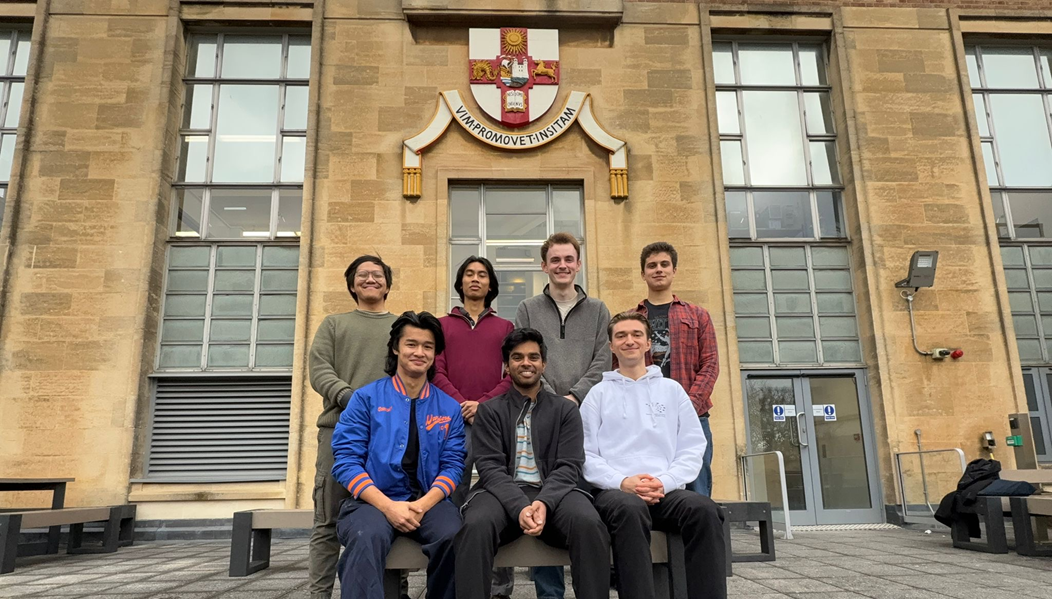
\includegraphics[width=\linewidth]{figures/group_photo.png}
\vspace{1.5em}

\begin{tabular}{ccc}
Nick Balboa & Romuald Saithanyan Christy Ruban & Alan Wawrzyńczok \\
\textit{Communications/OBDH} & \textit{Structures} & \textit{Power/Thermal} \\
\textit{University of Bristol} & \textit{University of Bristol} & \textit{University of Bristol} \\
Bristol, England & Bristol, England & Bristol, England \\
\textit{Email redacted} & \textit{Email redacted} & \textit{Email redacted} \\
\end{tabular}

\end{center}


\vfill
\end{titlepage}


% ---------------------------------------------------------------------------
% CONTENTS
% ---------------------------------------------------------------------------
\clearpage
\onecolumn
\renewcommand{\contentsname}{\large\bfseries CONTENTS}
\pagenumbering{roman}
\tableofcontents
\clearpage

% ---------------------------------------------------------------------------
% NOMENCLATURE  (own page, not in ToC)
% ---------------------------------------------------------------------------
\section*{Nomenclature}
\addcontentsline{toc}{section}{Nomenclature}

% helper
\newcommand{\nomentry}[3]{\noindent \textbf{#1}\;\; #2 \dotfill \par}

\nomentry{ADS-B}{Automatic Dependent Surveillance–Broadcast}{nom:adsb}
\nomentry{AIS}{Automatic Identification System}{nom:ais}
\nomentry{AIT}{Assembly, Integration and Testing}{nom:ait}
\nomentry{AOCS}{Attitude and Orbit Control System}{nom:aocs}
\nomentry{AVDASI}{Aerospace Vehicular Design and Systems Integration}{nom:avdasi}
\nomentry{BER}{Bit Error Rate}{nom:ber}
\nomentry{BOL}{Beginning of Life}{nom:bol}
\nomentry{BPSK}{binary phase-shift keying}{nom:bpsk}
\nomentry{BRL}{Bit Rate Loss}{nom:brl}
\nomentry{CAD}{Computer-Aided Design}{nom:cad}
\nomentry{CADE}{Civil, Aerospace and Design Engineering}{nom:cade}
\nomentry{CDR}{Critical Design Review}{nom:cdr}
\nomentry{CE}{Concurrent Engineering}{nom:ce}
\nomentry{CFRP}{Carbon-Fibre Reinforced Polymer}{nom:cfrp}
\nomentry{CG}{Center of Gravity}{nom:cg}
\nomentry{CMG}{Control Moment Gyroscope}{nom:cmg}
\nomentry{CONOPS}{Concept of Operations}{nom:conops}
\nomentry{COPV}{Composite Over-wrapped Pressure Vessel}{nom:copv}
\nomentry{COTS}{Commercial Off-The-Shelf}{nom:cots}
\nomentry{CTE}{Coefficient of Thermal Expansion}{nom:cte}
\nomentry{CVD}{Chemical Vapour Deposition}{nom:cvd}
\nomentry{DoD}{Depth of Discharge}{nom:dod}
\nomentry{DOT}{Department of Transportation}{nom:dot}
\nomentry{DRAMA}{Debris Risk Assessment and Mitigation Analysis}{nom:drama}
\nomentry{EIRP}{Effective Isotropic Radiated Power}{nom:eirp}
\nomentry{EOL}{End of Life}{nom:eol}
\nomentry{EPS}{Electrical Power System}{nom:eos}
\nomentry{ESA}{European Space Agency}{nom:ESA}
\nomentry{ESD}{Electrostatic Discharge}{nom:esd}
\nomentry{FCC}{Federal Communications Commission}{nom:fcc}
\nomentry{FDIR}{Fault Detection Isolation and Recovery}{nom:fdir}
\nomentry{FDR}{Final Design Review}{nom:fdr}
\nomentry{FEA}{Finite Element Analysis}{nom:fea}
\nomentry{FEDR}{Final Engineering Design Report}{nom:fedr}
\nomentry{FEP}{Fluorinated Ethylene Propylene}{nom:fep}
\nomentry{FIR}{Flight Information Region}{nom:fir}
\nomentry{FMEA}{Failure Modes and Effects Analysis}{nom:fmea}
\nomentry{GaAs}{Gallium Arsenide}{nom:gaas}
\nomentry{GMSK}{Gaussian Minimum Shift Keying}{nom:gmsk}
\nomentry{GNSS}{Global Navigation Satellite System}{nom:gnss}
\nomentry{GPS}{Global Positioning System}{nom:gps}
\nomentry{HPOP}{High Precision Orbit Propagator}{nom:hpop}
\nomentry{HTP}{High Test Peroxide}{nom:htp}
\nomentry{IMU}{Inertial Measurement Unit}{nom:imu}
\nomentry{ISP}{Specific Impulse}{nom:isp}
\nomentry{ITAR}{International Traffic in Arms Regulations}{nom:itar}
\nomentry{IOCR}{In-Orbit Commissioning Review}{nom:iocr}
\nomentry{IOM}{In-Orbit Manufacturing}{nom:iom}
\nomentry{IR}{Infrared}{nom:ir}
\nomentry{LAN}{Longitude of the Ascending Node}{nom:lan}
\nomentry{LEO}{Low Earth Orbit}{nom:leo}
\nomentry{LEOP}{Launch and Early Orbit Phase}{nom:leop}
\nomentry{LM}{Link Margin}{nom:lm}
\nomentry{LTAN}{Local Time of the Ascending Node}{nom:ltan}
\nomentry{MCDA}{Multi-Criteria Decision Analysis}{nom:mcda}
\nomentry{MRD}{Market Requirements Document}{nom:mrd}
\nomentry{MEOP}{Maximum Expected Operating Pressure}{nom:meop}
\nomentry{MPPT}{Maximum Power Point Tracking}{nom:mppt}
\nomentry{MTQ}{Magnetic Torquer / Magnetorquer}{nom:mtq}
\nomentry{MULASSIS}{Multi-Layer Shielding Simulation Analysis tool}{nom:mulassis}
\nomentry{Nom}{Nominal}{nom:nom}
\nomentry{NRLMSISE}{Naval Research Laboratory Mass Spectrometer and Incoherent Scatter Radar Exosphere}{nom:nrlmsise}
\nomentry{OAP}{Orbit Average Power}{nom:oap}
\nomentry{OBC}{On-Board Computer}{nom:obc}
\nomentry{OBDH}{On-Board Data Handling}{nom:obdh}
\nomentry{OSCAR}{Orbital SpaceCraft Active Removal}{nom:oscar}
\nomentry{CVD}{Chemical Vapour Deposition}{nom:cvd}
\nomentry{PCDU}{Power Conditioning and Distribution Unit}{nom:pcdu}
\nomentry{PDR}{Preliminary Design Review}{nom:pdr}
\nomentry{P\&ID}{Plumbing \& Instumentaion Diagram}{nom:pid}
\nomentry{QPSK}{Quadrature Phase-Shift Keying}{nom:qpsk}
\nomentry{RDT}{Rapid Data Transfer}{nom:rdt}
\nomentry{RF}{Radio Frequency}{nom:rf}
\nomentry{RPN}{Risk Priority Number}{nom:rpn}
\nomentry{RSL}{Receiver System Loss}{nom:rsl}
\nomentry{RW}{Reaction Wheels}{nom:rw}
\nomentry{SA}{Solar Array}{nom:sa}
\nomentry{SARA}{Re-entry Survival and Risk Analysis}{nom:sara}
\nomentry{SCIPIO}{Semi-Conductor Industrial Processing In Orbit}{nom:scipio}
\nomentry{SMAD}{Space Mission Analysis and Design}{nom:smad}
\nomentry{SND}{System Noise Density}{nom:snd}
\nomentry{SPENVIS}{Space Environment Informaation System}{nom:spenvis}
\nomentry{SPOUA}{South Pacific Oceanic Uninhabited Area}{nom:spoua}
\nomentry{SSO}{Sun–Synchronous Orbit}{nom:sso}
\nomentry{STK}{Systems Tool Kit}{nom:stk}
\nomentry{SEET}{System End-To-End Testing}{nom:seet}
\nomentry{SEET}{Space Environment And Effects Tool}{nom:seet_stk}
\nomentry{SEU}{Single Event Upset}{nom:seu}
\nomentry{TID}{Total Ionising Dose}{nom:tid}
\nomentry{TRL}{Technology Readiness Level}{nom:trl}
\nomentry{TT\&C}{Telemetry, Tracking and Command}{nom:tt&c}
\nomentry{TVAC}{Thermal Vacuum}{nom:tvac}
\nomentry{UHF}{Ultra High Frequency}{nom:uhf}
\nomentry{VHF}{Very High Frequency}{nom:vhf}
\newpage
\setlength{\parskip}{0.8em} % remove first "%" to add paragraph spacing
\setlength\parindent{0pt}

% ---------------------------------------------------------------------------
% REQUIREMENTS (front-matter section, as in outline)
% ---------------------------------------------------------------------------
\section*{Objectives}
\addcontentsline{toc}{section}{Objectives}
\label{sec:obj}

\begin{table}[H]
\centering
\caption{Space Forge Objectives}
\label{tab:spaceforge-objs}
\footnotesize
\renewcommand{\arraystretch}{1.2}
\begin{tabular}{@{}p{0.15\linewidth}p{0.80\linewidth}@{}}
\toprule
\textbf{Objective ID} & \textbf{Objective} \\
\midrule
OBJ-01 & Fly and run the in-orbit manufacturing payload for its required operational time \\
OBJ-02 & Measure the microgravity levels inside the main structures \\
OBJ-03 & Measure the ambient pressure inside the main structure \\
OBJ-04 & Take a picture of Earth with part of the satellite in view \\
OBJ-05 & Targeted destructive re-entry within a specified landing zone \\
\bottomrule
\end{tabular}
\end{table}
\normalsize



\section*{Requirements}
\addcontentsline{toc}{section}{Requirements}
\label{sec:req}

Table~\ref{tab:spaceforge-reqs} contains all Space Forge Requirements as defined in the AVDASI 4 Mission Requirements Document~\cite{williams_avdasi_2025}.

{\footnotesize
\renewcommand{\arraystretch}{1.2}
\begin{longtable}{@{}p{0.15\linewidth}p{0.80\linewidth}@{}}
\caption{Space Forge Requirements}
\label{tab:spaceforge-reqs} \\

\toprule
\textbf{Requirement ID} & \textbf{Requirement} \\
\midrule
\endfirsthead

\toprule
\textbf{Requirement ID} & \textbf{Requirement} \\
\midrule
\endhead

SFG-REQ-010 & The satellite shall be capable of supporting a mission operation of up to 2~years, excluding commissioning and decommissioning. \\
SFG-REQ-020 & The satellite shall fit within a $1200 \times 700 \times 700\,\mathrm{mm}$ volume. \\
SFG-REQ-030 & The satellite shall be compatible with the Falcon~9 launch system. \\
SFG-REQ-040 & The satellite shall be compatible with the Ariane~6 launch system. \\
SFG-REQ-050 & The satellite shall be compatible with the Electron launch system. \\
SFG-REQ-060 & The satellite shall have a maximum wet mass of $40\,\mathrm{kg}\pm 2\,\mathrm{kg}$. \\
SFG-REQ-070 & The satellite shall accommodate the payload provided by Space Forge, as defined in the payload specification (see Section~3.2 of the Mission Requirements Document). \\
SFG-REQ-080 & The satellite shall have at least one anchor point to allow lifting of the whole spacecraft for transport and integration purposes. \\
SFG-REQ-090 & The satellite shall de-orbit within 25~years under all scenarios, including if the system is dead on release from the launcher. \\
SFG-REQ-100 & Any debris released by the satellite shall de-orbit within 5~years. \\
SFG-REQ-110 & If performing a destructive re-entry, the satellite shall be completely destroyed with no debris surviving to reach Earth's surface. \\
SFG-REQ-120 & The satellite shall protect against radiation damage resulting in the failure of a critical system up to a total ionising dose (TID) of $16~\mathrm{krad}$ over a 2~year orbital lifetime. \\
SFG-REQ-130 & The satellite should protect against radiation damage resulting in the failure of non-critical systems up to a total ionising dose (TID) of $16~\mathrm{krad}$ over a 2~year orbital lifetime. \\
SFG-REQ-140 & The satellite shall have a microgravity sensor within 100~mm of the payload. \\
SFG-REQ-150 & The satellite should offer a $< 1 \times 10^{-4}\,\mathrm{g}$ gravity environment to the payload when averaged over a 14~day period during the primary mission phases. \\
SFG-REQ-160 & The satellite shall have an internal pressure sensor within 100~mm of the payload. \\
SFG-REQ-170 & The satellite shall provide a vacuum environment of $< 1$~mPa to the payload. \\
SFG-REQ-180 & The satellite shall have a defined safe mode where all non-critical operations are disabled. \\
SFG-REQ-190 & The satellite shall be able to determine its position to $< 10$~m and velocity to $< 1\,\mathrm{m\,s}^{-1}$ during all mission phases. \\
SFG-REQ-200 & The satellite shall provide real-time satellite location and velocity to the ground team when commanded. \\
SFG-REQ-210 & The satellite should have an independent timing source to synchronise internal (satellite) operations. \\
SFG-REQ-220 & The satellite shall be able to detumble from a worst-case tumbling of $2^\circ$\,s$^{-1}$ in a single axis. \\
SFG-REQ-230 & The satellite shall be capable of capturing a visual image of the Earth with part of the satellite in the field of view. \\
SFG-REQ-240 & The satellite should generate power for all platform and payload operations from solar energy. \\
SFG-REQ-250 & The satellite shall support full duplex communication. \\
SFG-REQ-260 & The satellite and the ground segment shall offer communication passes of at least 5~minutes at least once every 12~hours. \\
SFG-REQ-270 & During a communication pass, the satellite and the ground segment shall support the uplink of payload telecommands at a minimum rate of 1~command per second. \\
SFG-REQ-280 & The operations team shall be able to download a log of all satellite platform telemetry at least once every 24~hours. \\
SFG-REQ-290 & The satellite shall downlink platform critical telemetry at least once every 4~hours during all mission phases. \\
SFG-REQ-300 & When the payload is powered on, the operations team shall be able to download all newly accumulated data generated by the payload at least once every 24~hours. \\
SFG-REQ-310 & When the payload is powered on, the payload critical telemetry packet shall be downlinked at least once every 2~hours. \\
SFG-REQ-320 & During payload operation, the satellite shall maintain the payload inertially fixed with a maximum allowed deviation of $1^\circ$ per 24~hours. \\
SFG-REQ-330 & When commanded, the satellite shall be able to downlink any images taken by the payload. \\
SFG-REQ-340 & The satellite shall ensure that the payload's positive Y face is exposed and accessible during AIT. \\
SFG-REQ-350 & The satellite shall ensure that the payload's positive Y face is exposed to space during payload operation. \\
\bottomrule

\end{longtable}
}

\vspace{5pt}

The table below includes all requirements derived by SerenSpace. The requirement index indicates from which Space Forge requirement the requirement has been derived - i.e. an index of the form "-03X" indicates the requirement is derived from SFG-REQ-030.

\begin{table}[H]
\centering
\caption{SerenSpace Derived Requirements}
\label{tab:serenspace-reqs}
\footnotesize
\renewcommand{\arraystretch}{1.2}
\begin{tabular}{@{}p{0.15\linewidth}p{0.80\linewidth}@{}}
\toprule
\textbf{Requirement ID} & \textbf{Requirement} \\
\midrule
THM-REQ-011 & The payload shall maintain a safe operational temperature for all its constituent components. \\
SAT-REQ-031 & The stowed satellite shall fit within the SpaceX 1/4 plate volume envelope. \\
SAT-REQ-032 & The satellite centre of mass shall lie within $400\,\mathrm{mm}$ of the satellite origin, as defined in the Falcon Rideshare User Guide. \\
SAT-REQ-033 & The satellite shall be able to withstand all launch loads, in accordance with the Falcon, Ariane and Electron User Guides. \\
SAT-REQ-034 & The satellite shall include a standard 8" separation ring. \\
PRP-REQ-035 & All pressure vessels shall either receive US DOT certification or be designed and qualified to safety factors defined in Table 5-6 of the Falcon 9 Rideshare User Guide. \\
PRP-REQ-036 & Pressure vessels shall have contingency pressure release to vent pressure above MEOP. \\
PRP-REQ-037 & All valves/fittings/regulators shall comply with pressure safety factors outlined in Table 5-6 of the Falcon 9 Rideshare User Guide. \\
PRP-REQ-038 & The Propulsion System shall be at least single fault tolerant to pressure release. \\
MIS-REQ-039 & The satellite shall deorbit within 5~years of the mission end, in accordance with FCC-22-74 and the Falcon 9 User Guide. \\
PLM-REQ-071 & The satellite shall allocate a volume of 340x100x100~mm to the payload, with mounting holes according to the payload ICD. \\
PLT-REQ-072 & The satellite shall maintain the payload temperature between $-35^\circ\,\mathrm{C}$ and $+85^\circ\,\mathrm{C}$. \\
PLP-REQ-073 & The satellite shall provide $10\,\mathrm{W}$ to the payload when in "operational" mode. \\
PLP-REQ-074 & The satellite shall provide $80\,\mathrm{W}$ to the payload for a 10-minute period every 24~hours. \\
PLP-REQ-075 & The satellite shall provide $1\,\mathrm{W}$ to the payload when in "idle" mode. \\
PLO-REQ-076 & The satellite shall be kept in "operational" mode for at least 6 months in orbit. \\
PLO-REQ-077 & The payload shall be maintained in ``idle" for a minimum of two weeks prior to regular operation, for commissioning. \\
AOC-REQ-001 & The AOCS shall be able to counteract any torque produced by thruster misalignment, with a suitable margin. \\
\bottomrule
\end{tabular}
\end{table}

\normalsize
\clearpage
\pagenumbering{arabic}




% High-level requirement list can go here.
% Detailed requirement tables can be moved to an Appendix if preferred.

\clearpage
\pagenumbering{arabic}


% ---------------------------------------------------------------------------
% 1. EXECUTIVE SUMMARY
% ---------------------------------------------------------------------------
%\twocolumn
\section{Executive Summary}

Space Forge is a New Space \cite{rementeria_power_2022} company based in Cardiff, UK, focused on advanced material manufacturing in orbit. Space Forge’s first In-Orbit Manufacturing (IOM)\label{nom:iom} payload utilises Chemical Vapour Deposition (CVD)\label{nom:cvd} processes to manufacture high-quality semiconductor crystals. The SCIPIO-1 mission will demonstrate and validate this payload by providing the low-pressure microgravity environment it needs to operate. It will be the first in a line of missions with the eventual goal of commercial semiconductor manufacturing in-orbit.

SCIPIO-1 has been designed to operate in a $520\,\mathrm{km}$ mid-morning Sun-Synchronous Orbit (SSO)\label{nom:sso} in order to maximise launch opportunities on commercial rideshare missions, while eliminating the need for high-risk orbit injection manoeuvres. This orbit ensures compliance with both the customer's pressure (SFG-REQ-170) and dead-on-release deorbit (SFG-REQ-090) requirements. No station keeping manoeuvres are planned during the mission, as these were deemed an unnecessary risk. At the End of Life (EOL)\label{nom:eol}, the satellite will perform a controlled deorbit burn to comply with Space Forge's deorbit objective (OBJ-05). A target re-entry region in the South Pacific Oceanic Uninhabited Area (SPOUA)\label{nom:spoua} has been selected to mitigate ground risks associated with incomplete burn-up.

The communications architecture for the mission separates downlink opportunities into critical and non-critical telemetry, due to the differing cadence requirements for each (SFG-REQ-280/290/300/310). UHF\label{nom:uhf} will be utilised for the small volumes of critical data, due to its wide coverage and reliability \cite{ippolito_satellite_2017}, whilst S-band will transmit the bulk telemetry. Terran-Orbital's ground station network has been selected, after mission analysis found that it could offer access opportunities every orbit over UHF. This ensures the mission can meet requirements SFG-REQ-290 and SFG-REQ-310. The network also features three S-band ground stations which are capable of comfortably meeting the satellite's downlink requirements. To implement this architecture, the communications subsystem will feature two UHF dipole antennas and two S-band patch antennas, each placed on opposite faces to maximise coverage. Each UHF antenna will be accompanied by its own half-duplex transceiver, whilst a single full-duplex S-band transceiver will serve both S-band antennas.

The satellite itself has a wet mass of $41.3\,\mathrm{kg}$, with ESA margins applied \cite{noauthor_sre-pa2011097_2012}, and occupies a volume of $850\times500\times400\,\mathrm{mm}$. This ensures the satellite fits within the Falcon 9 quarter-plate volume envelope. Structurally, the satellite utilises Carbon-Fibre Reinforced Polymer (CFRP)\label{nom:cfrp} due to its high stiffness to weight ratio. A central cylinder, surrounded by four shear webs, will act as the primary load-bearing structure, with interior shelves to mount equipment and reinforce the outer panels. Exterior coatings both mitigate the effects of atomic oxygen and provide passive thermal control. Further thermal control will be provided by distributed polyimide heaters, and heat pipes to evenly distribute heat.

Power will be generated by a combination of body-mounted and deployable solar panels, each utilising multijunction gallium arsenide cells. Combined, these will be capable of generating a peak power of $308\,\mathrm{W}$ at BOL\label{nom:bol}. Two PCDUs\label{nom:pcdu}, each with MPPT\label{nom:mppt} functionality, have been implemented to regulate and distribute this power to the rest of the satellite, with the second providing hot redundancy. To handle both periods spent in eclipse and the power deficit during propulsive manoeuvres, a $432\,\mathrm{W\,h}$ lithium-ion battery has been included for power storage.

Attitude control is achieved with reaction wheels and magnetorquers, whilst star trackers, sun sensors, GNSS\label{nom:gnss} receivers, a magnetometer and an IMU\label{nom:imu} provide sensing. These enable inertial pointing (SFG-REQ-320) and are capable of maintaining microgravity accelerations below $10^{-4}\,\mathrm{g}$ for the payload (SFG-REQ-150). To meet Space Forge’s targeted re-entry objective, SCIPIO-1 will feature a hydrazine-based propulsion system, with a single $5\,\mathrm{N}$ thruster. A budgeted delta-V of $145.7\,\mathrm{m\,s}^{-1}$ facilitates both deorbit and collision avoidance manoeuvres.

By adopting a heritage-driven design philosophy, SCIPIO-1 represents a pragmatic, low-risk design capable of fulfilling all of Space Forge's mission objectives.

\onecolumn
\clearpage

\section{Spacecraft Datasheet}
\begin{tabular}{p{0.25\linewidth} p{0.7\linewidth}}
\hline
\multicolumn{2}{c}{\textbf{Mission Overview}} \\
\hline
Mission Aim & Demonstrate and validate Space Forge's CVD Payload \\
Payload & Space Forge CVD Semiconductor Manufacturing Unit \\
Launch & SpaceX Falcon 9 Transporter, June 2027\\
Orbit & Sun-Synchronous Orbit (SSO)\\
LTAN & 10:30 \\
Altitude & 520km \\
Deorbit plan & Targeted destructive re-entry into the SPOUA\\
Operational Modes & Science Mode, Safe Mode, Collision Avoidance Mode, Rapid Data Transfer Mode \\
Design Lifetime & 2 years \\
\hline
\multicolumn{2}{c}{\textbf{Configuration}} \\
\hline
Wet Mass & $41.0\,\mathrm{kg}$ \\
Dimensions & $500\times400\times850\,\mathrm{mm}$ \\
Center of Mass & X: -$8.23\,\mathrm{mm}$ Y: $8.87\,\mathrm{mm}$ (Stowed) $-2.69\mathrm{mm}$ (Deployed) Z: $346.37\,\mathrm{mm}$ \\
\hline
\multicolumn{2}{c}{\textbf{Thermal}} \\
\hline
Hardware & 8 x Polyimide Heaters, Passive Coatings, Thermistors, Heat Pipes \\
Temperature Limits &  Cold Case: $-55^\circ\,\mathrm{C}$ Hot Case: $44^\circ\,\mathrm{C}$\\
\hline
\multicolumn{2}{c}{\textbf{AOCS}} \\
\hline
Actuators &  3 Magnetorquers, 4 Reaction Wheels\\
Sensors &  2 Star Trackers, 2 Fine Sun Sensors, IMU, Magnetometer, 2 GNSS Recievers and Antennas\\
\hline
\multicolumn{2}{c}{\textbf{Propulsion}} \\
\hline
Delta-V &  $145.7\,\mathrm{m\,s}^{-1}$ (Deorbit and  Collision Avoidance)\\
Hardware & Rafael $5\,\mathrm{N}$ Thruster, PBT-3 Hydrazine Bladder Tank, Nitrogen COPV Tank\\
Propellant \& Pressurant &  $2.66\,\mathrm{kg}$ Hydrazine at $24\,\mathrm{bar}$, $0.12\,\mathrm{kg}$ Nitrogen at $110\,\mathrm{bar}$\\
Thrust &  $4.7\,\mathrm{N}$ maximum\\
\hline
\multicolumn{2}{c}{\textbf{Power}} \\
\hline
Power Generation & Multi-juncition GaAs Solar Cells  \\
Configuration & 2 Deployable ($2\times79$ Cells), +Y Body-Mounted (84 Cells), -Y Body-Mounted (70 Cells)\\
Max Power Generation & $308\,\mathrm{W}$ (Safe Mode)\\
Power Storage & $432\,\mathrm{W\,h}$ Li-ion Battery \\
Distribution & Primary + Redundant Bradford Space Supernova PCDUs \\
Power Budget & Science Mode: OAP Generation: 169W, OAP Draw: 93W \\
\hline
\multicolumn{2}{c}{\textbf{Communications}} \\
\hline
Ground Station &  Terran Orbital Ground Station Network \\ 
Uplink Frequencies & UHF: $400\,\mathrm{MHz}$, S-band: $2075\,\mathrm{MHz}$\\
Downlink Frequencies & UHF: $400\,\mathrm{MHz}$, S-band: $2250\,\mathrm{MHz}$\\
Hardware & UHF: 2$\times$Spacemanic Dipole Antennas, 2$\times$Spacemanic Transceivers 

S-band: 2$\times$Anywaves TT\&C Antenna, 1$\times$Slink-PHY Transceiver
 \\
Link Margins (dB) &\begin{tabular}{ c c c c }
  & UHF & S-Band (Nom) & S-band (RDT) \\ 
 Uplink & 17.2 & 10.2& 18.2  \\   
 Downlink & 11.1 & 6.5 & 6.3\\  
\end{tabular} 
 \\
\hline
\multicolumn{2}{c}{\textbf{Structures}} \\
\hline
Material & CFRP (Hexcel IM7/8552), Hexcel CRIII 5052 Honeycomb Core, Al 6061-T6 \\
Arrangement & Central Tapered Cylinder, 4 Shear Webs, 2 Shelves, Exterior Panels  \\
\hline
\end{tabular}

% ---------------------------------------------------------------------------
% 3. GENERAL ARRANGEMENT
% ---------------------------------------------------------------------------
\section{General Arrangement}
\vspace{-15pt}
\noindent\hspace{-15pt}\makebox[\textwidth][c]{%
  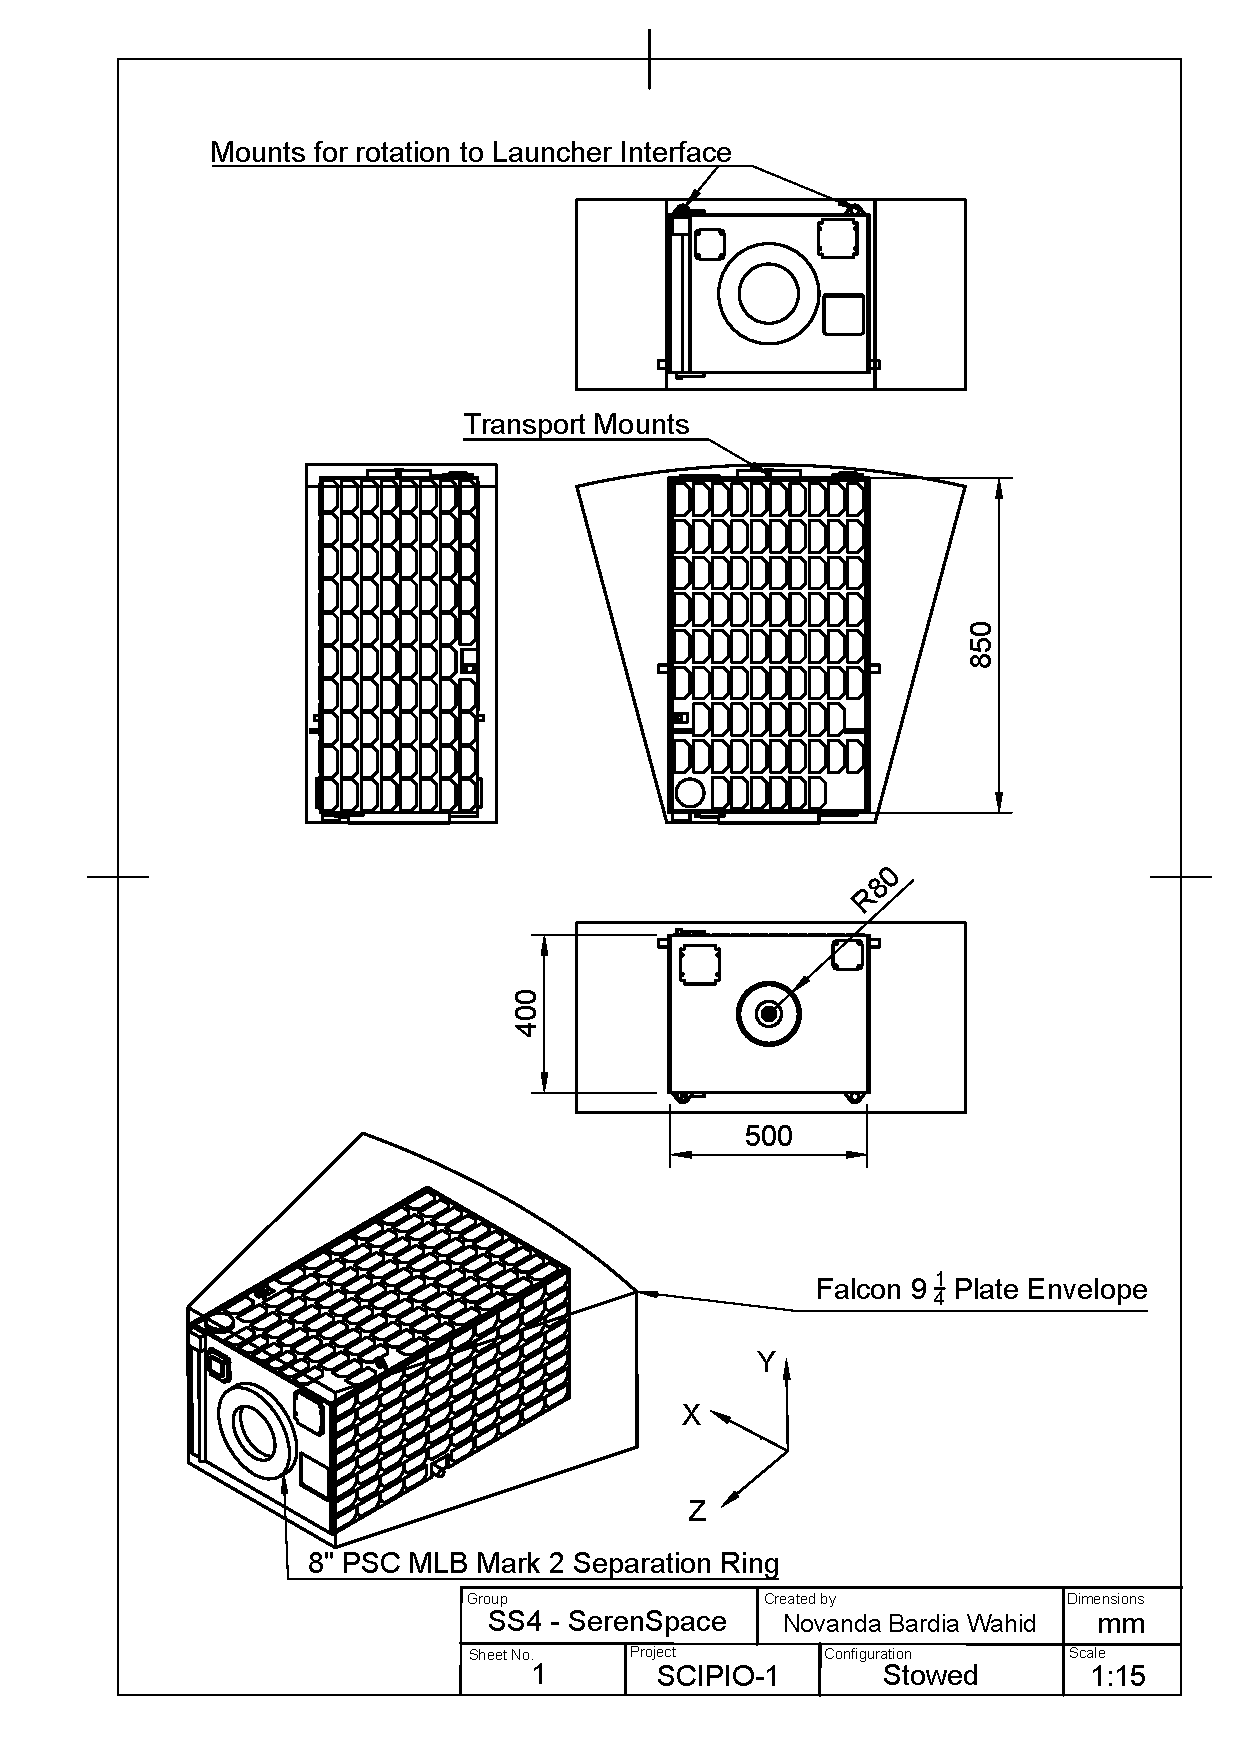
\includegraphics[
    width=0.9\linewidth,
    keepaspectratio
    ]{figures/spacecraft_stowed_drawing.pdf}%
}

\newpage
\noindent\hspace{-15pt}\makebox[\textwidth][c]{
  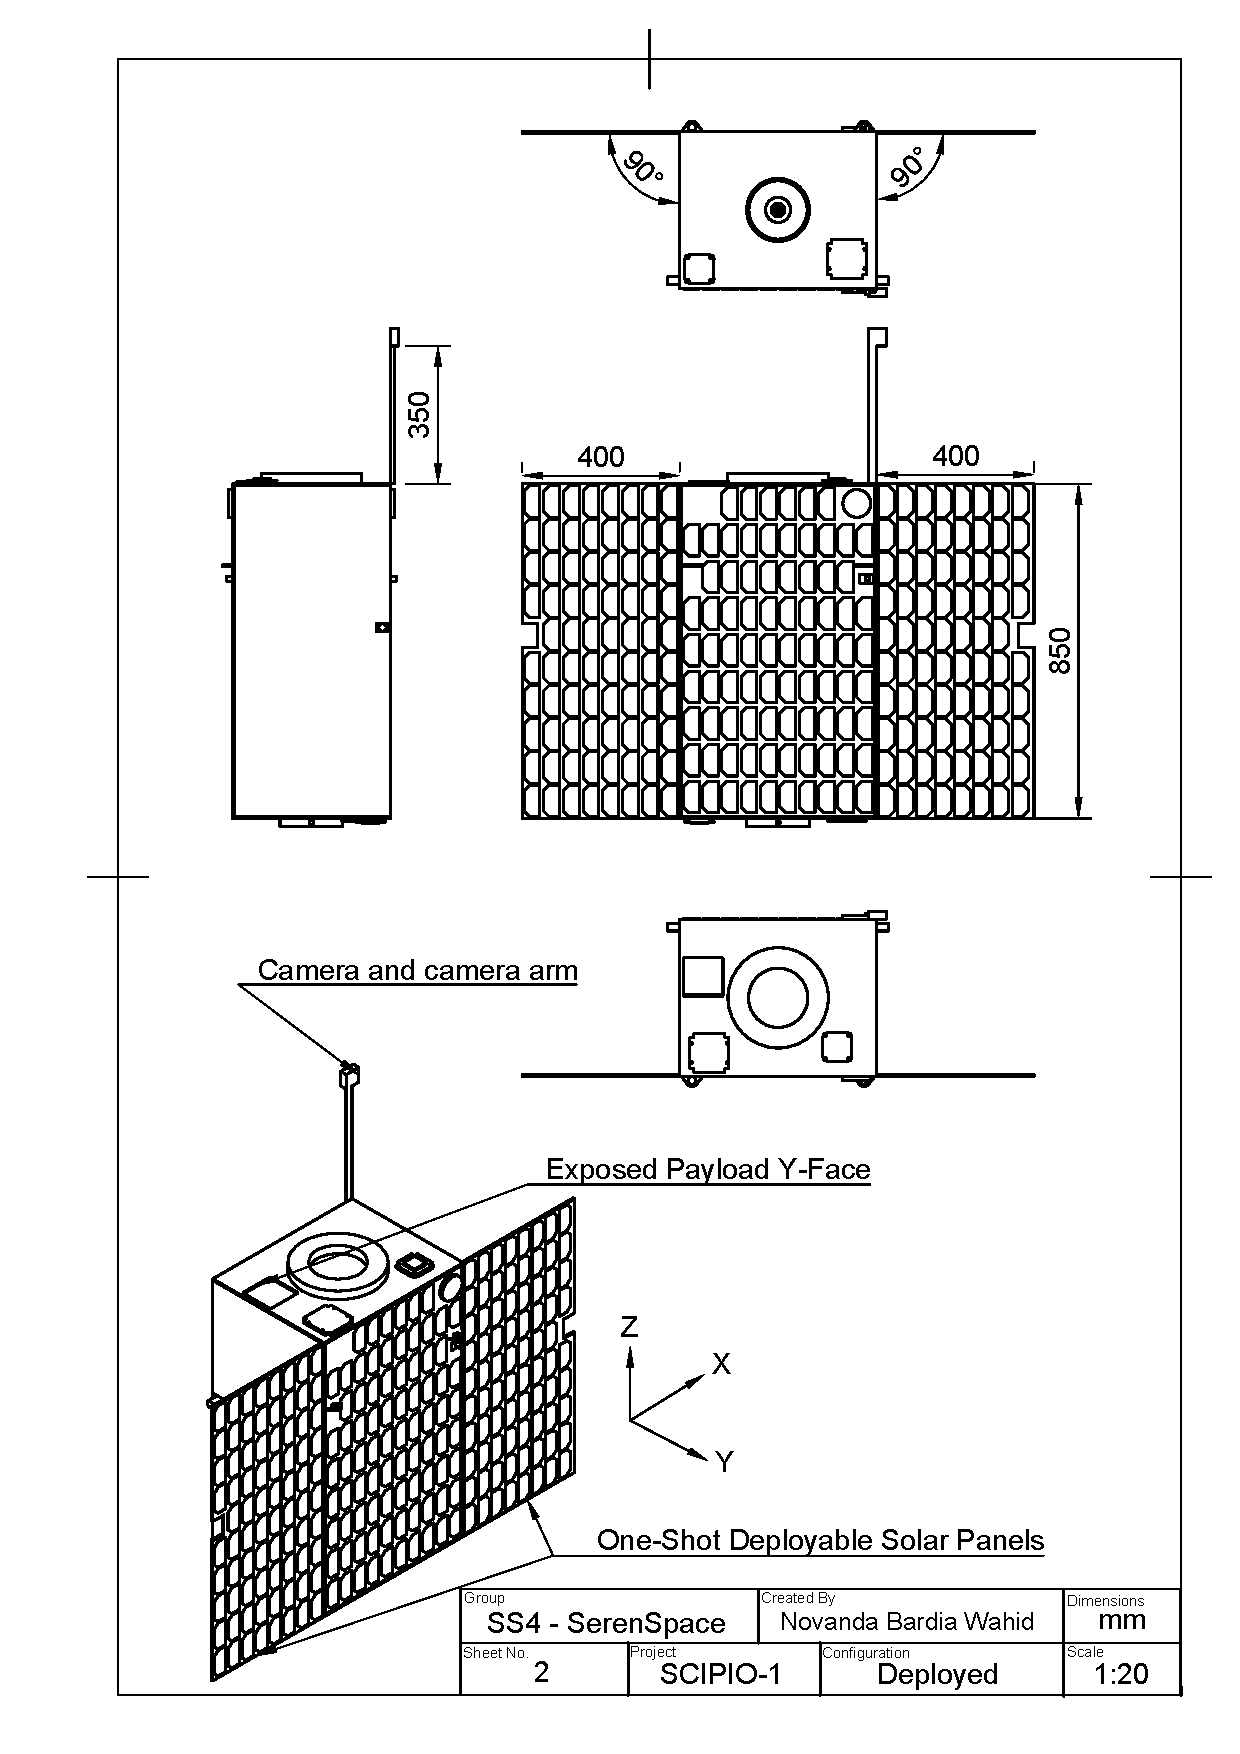
\includegraphics[
    width=0.9\linewidth,
    keepaspectratio
  ]{figures/spacecraft_deployed_drawing.pdf}%
}

% ---------------------------------------------------------------------------
% 4. MISSION OVERVIEW
% ---------------------------------------------------------------------------
\newpage
\section{Mission Overview and Analysis}
% As per outline: covers objectives, requirements, drivers, etc.
Space Forge's Chemical Vapour Deposition (CVD) payload has been developed to exploit the space environment for its unique manufacturing potential. By operating in a low-pressure, microgravity environment, the payload has the potential to produce semiconductor crystals with purities 2–4 orders of magnitude higher than those produced terrestrially \cite{williams_avdasi_2025}. The SCIPIO-1 mission provides Space Forge with an orbital platform to both demonstrate and validate this payload (OBJ-01), marking the first step in achieving commercial semiconductor manufacturing on orbit. Following a 2-year mission lifetime, SCIPIO-1 will perform a controlled, destructive re-entry into the South Pacific Oceanic Uninhabited Area (SPOUA) to fulfil OBJ-05. Though the payload will not be returned intact for this mission, the planned propulsive deorbit manoeuvre will serve as a proof of concept for targeted re-entry, with future missions utilising Space Forge's Pridwen heat shield \cite{noauthor_space_2025} for payload recovery.
\vspace{-10pt}
\subsection{Mission Requirements and Drivers}

During the initial phases of the project, the customer's requirements were assessed to understand their impact on the system design. ``Critical" requirements were defined as those for which non-compliance would lead to the direct failure of a customer mission objective. Among these critical requirements, a selection were identified as ``driving", owing to their influence on multiple aspects of system design and their relative importance. These are summarised in Table~\ref{tab:critical_driving_reqs}, along with rationale and associated design impacts.

\begin{table}[H]
\caption{Driving Critical Requirements}
\label{tab:critical_driving_reqs}
\centering
\begin{tabularx}{\linewidth}{l X|X} % ← vertical line added here
\toprule
\textbf{Req. ID} & \textbf{Rationale} & \textbf{Drives} \\
\midrule

SFG-REQ-010 & 
Overarching requirement ensuring safe operation in space for the required lifetime.
& All aspects of mission design. \\

SFG-REQ-030 & 
This, and its derived requirements, ensure that the satellite can be launched into the required orbit. 
& Spacecraft configuration, structural design, orbit selection, concept of operations. \\

SFG-REQ-070 &
Encapsulates the primary mission objective. Failure to satisfy it, or any of its derived requirements, would result in automatic non-compliance with OBJ-01. 
& All aspects of system and mission design. \\

SFG-REQ-150 & 
Ensures the payload is provided the correct operating conditions - the primary motivation for utilising space.
& Orbit selection, AOCS design, CONOPS. \\

SFG-REQ-170 & 
Another primary motivation for utilising space. Failure to comply means the payload cannot be activated, resulting in mission failure. 
& Orbit selection. \\

SFG-REQ-220 &
Ensures the satellite can enter into its nominal ops phase following LEOP\label{nom:leop}, enabling payload activation. 
& AOCS design, CONOPS. \\

SFG-REQ-240 &
Ensures power can be supplied to subsystems in all mission phases and modes. 
& Orbit selection, configuration, power subsystem design. \\

SFG-REQ-290 &
Ensures that the platform health can be monitored and faults mitigated in a timely manner. 
& Communications design, OBDH design, ground station selection. \\

SFG-REQ-300 &
Since payload recovery is not planned, payload data is the primary output of the mission. Failure to comply means the payload cannot be validated. 
& Communications design, OBDH design, orbit selection, ground station selection. \\

SFG-REQ-310 &
Ensures that the payload health can be monitored and anomalies detected in a timely manner. 
& Communications design, OBDH design, orbit selection, ground station selection. \\

SFG-REQ-320 &
Ensures the platform provides a suitable operational environment for the payload.
& Orbit selection, AOCS design, satellite configuration, CONOPS. \\

\bottomrule
\end{tabularx}
\end{table}
\vspace{0pt}
\subsection{Mission Analysis}

To evaluate candidate orbits, a trade study was carried out, utilising both a pairwise comparison and an MCDA\label{nom:mcda} matrix. Initially a dawn-dusk sun-synchronous orbit scored highest, due to its high power generation potential and thermal stability. However, further research into commercial rideshare missions revealed that access to such orbits was limited. Falcon 9, which was selected as primary launch vehicle due to its high reliability and low cost, was found to launch primarily to mid-morning and mid-afternoon SSOs.  Although slow LTAN\label{nom:ltan} phasing manoeuvres were considered, these were ruled out as they significantly increase mission risk and delay payload activation. To reflect these practical constraints, the pairwise comparison was updated, giving greater weighting to orbit accessibility; this led to the selection of a mid-morning SSO. The final orbit trade study is included in Appendix~\ref{subsec:orbit_downselection}.

Power generation, communications coverage and environmental perturbations were all weighted highly in the initial pairwise comparison, so maximisation of orbit altitude was deemed desirable. However, selection was constrained somewhat by the Falcon 9 Rideshare User Guide \cite{noauthor_falcon9rideshare_2024}, which mandates that spacecraft must comply with the FCC's 5-year deorbit requirement \cite{noauthor_fcc_2022}. An altitude of $520\,\mathrm{km}$ was therefore selected as this was the maximum achievable altitude whilst still ensuring deorbit within 5~years of mission end - even in the event of propulsion failure. Neither orbit injection nor station-keeping manoeuvres will be performed during the mission, to eliminate propulsion-related risk and maximise payload operating time. Although the customer's vacuum requirement (SFG-REQ-170) was considered critical, it had minimal impact on the design, as detailed in Section~\ref{sub:Miss_Anal_TR}.

\begin{table}[H]
    \centering
    \caption{Final Design Orbit Parameters}
    \begin{tabularx}{0.6\linewidth}{l c c c c c}
        \toprule
         & \textbf{Orbit Type} 
         & \textbf{LTAN} 
         & \textbf{Altitude (km)} 
         & \textbf{SMA (km)} 
         & \textbf{Inclination ($^\circ$)} \\
        \midrule
        \textbf{Value} 
         & SSO 
         & 10:30 
         & 520 
         & 6898
         & 97.5 \\
        \bottomrule
    \end{tabularx}
    \label{tab:Orbit_Params}
\end{table}


\vspace{-10pt}
To satisfy Space Forge's deorbit objective (OBJ-05),  SCIPIO-1 is planned to perform a targeted re-entry manoeuvre at the end of life. Though initially the Iceland's BIRD Flight Information Region (FIR)\label{nom:bird} was identified as a strategic re-entry corridor, this was ruled out after demisability analysis revealed that the satellite will not burn up completely upon re-entry (See Section~\ref{sub:Miss_Anal_TR}). The target region was thus moved to the SPOUA, due to its extreme remoteness and heritage as a spacecraft re-entry region \cite{ESA_reentry_2017}. Taking a worst-case scenario of a maximum separation altitude and ``low" solar and geomagnetic activity \cite{noauthor_ecss-e-st-10-04c_nodate}, a delta-V of $130.5$\,ms$^{-1}$ was estimated for this manoeuvre using DRAMA's OSCAR~\cite{noauthor_drama_nodate} tool. Due to the large area, approximately 6 deorbit opportunities are expected per day.



% ---------------------------------------------------------------------------
% 5. CONCEPT OF OPERATIONS
% ---------------------------------------------------------------------------
\section{Concept of Operations}
Launching on Falcon 9 in June 2027, SCIPIO-1 will separate at a nominal altitude of $520\,\mathrm{km}$. A separation switch will initiate a delayed power-on sequence, before the AOCS\label{nom:aocs} is activated to detumble the spacecraft. Afterwards, UHF antennas and solar panels will be deployed, and initial ground contact established. Once the satellite achieves a stable sun-pointing attitude, the payload will be powered on in ``idle" for a minimum of two weeks for commissioning, in accordance with PLO-REQ-077. Following an In-Orbit Commissioning Review (IOCR)\label{nom:iocr}, the satellite will enter into its nominal operations phase, in which it will operate in one of four modes:

\textbf{Science Mode:}
The default operating mode, with the payload ``operational". The satellite will maintain an inertially-fixed attitude, with a sun alignment, to comply with SFG-REQ-320. Magnetorquers will be used as the primary actuator to minimise microvibrations. Both UHF and S-band communications will be active.

\textbf{Safe Mode}:
Following an FDIR\label{nom:fdir} event or violation of payload operating limits, the satellite will transition to a sun-pointing safe mode to maximise power generation. The AOCS will continue to use magnetorquers as primary actuators both to minimise power draw and to allow ambient disturbance torques to be assessed. S-band transmission will be suspended to further minimise power consumption.

\textbf{Collision Avoidance Mode}:
In the event of a conjunction warning, the payload will be switched to ``idle" and the satellite slewed to align the thrusters with the manoeuvre direction. A propulsive manoeuvre will then be performed.

\textbf{Rapid Data Transfer (RDT)\label{nom:rdt} Mode}:
In the event of a ground command or the on-board data store exceeding $80\%$ capacity, the satellite will switch the payload to ``idle", and ground-track a ground station. This will enable both longer passes and higher data rates.


At the end of the 2-year mission lifetime, the satellite will perform a propulsive, targeted re-entry into the SPOUA.

% ---------------------------------------------------------------------------
% 6. SUBSYSTEM DESIGN (architecture, concept selection, final design)
% ---------------------------------------------------------------------------
\section{System Design}
\subsection{System Architecture}

\begin{figure}[H]
    \centering
    \resizebox{0.8\linewidth}{!}{%
        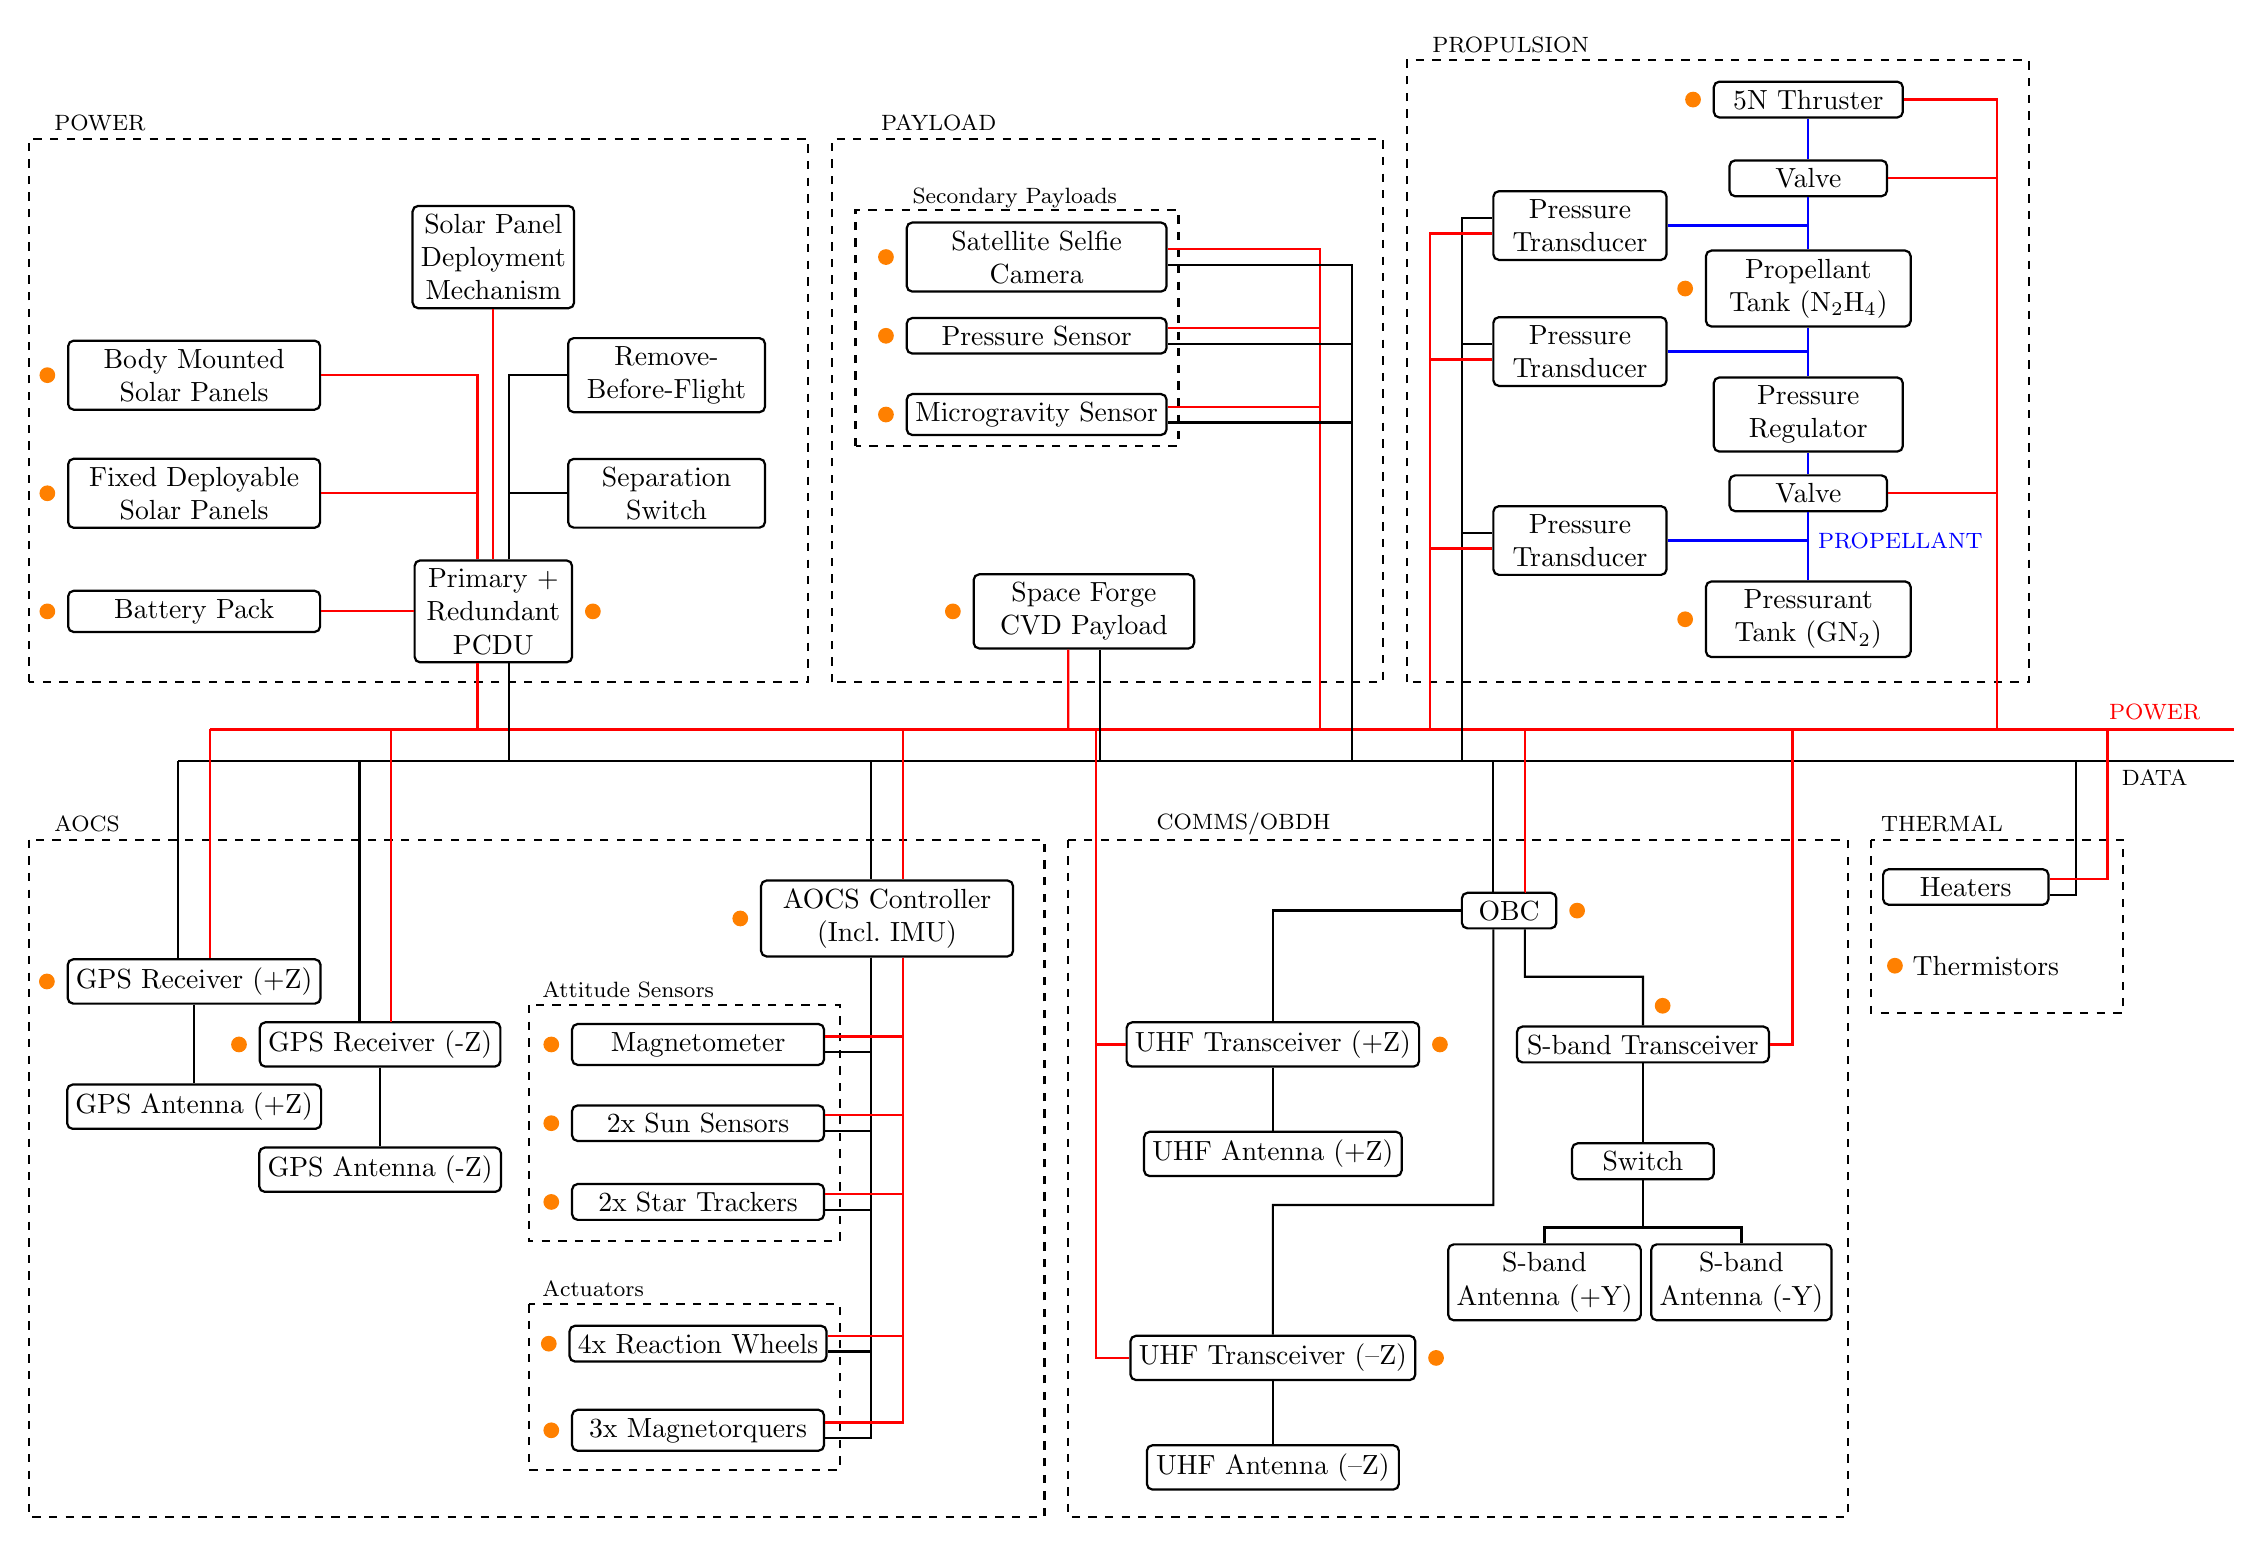
\begin{tikzpicture}

% RAILS
% Power
\draw[rail, red] (-0.1,0) -- (25.6,0);
\node[labelstyle, above, red] at (24.6,0) {POWER};

% Data
\draw[rail] (-0.5,-0.4) -- (25.6,-0.4);
\node[labelstyle, below] at (24.6,-0.4) {DATA};

% AOCS
\draw[dashed, thick] (-2.4,-1.4) rectangle (10.5,-10);
\node[labelstyle, anchor=west] at (-2.2,-1.2) {AOCS};

\node[box, minimum width=3.0cm] (gpsZ) at (-0.3,-3.2) {GPS Receiver (+Z)};

\draw[red, thick] (-0.1,0) |- ([xshift=0.2cm]gpsZ.north);
\draw[thick]      (-0.5,-0.4) |- ([xshift=-0.2cm]gpsZ.north);

\node[box, minimum width=3.0cm,
      right=-0.8cm of gpsZ,
      yshift=-0.8cm] (gpsZm) {GPS Receiver (-Z)};

\draw[red, thick] (2.2,0) |- ([xshift=0.15cm]gpsZm.north);

\draw[thick]      (1.8,-0.4) |- ([xshift=-0.25cm]gpsZm.north);

\node[box, minimum width=3.0cm,
      below=1cm of gpsZ] (gpsZ_ant) {GPS Antenna (+Z)};

\node[box, minimum width=3.0cm,
      below=1cm of gpsZm] (gpsZm_ant) {GPS Antenna (-Z)};

\draw[thick] (gpsZ.south) -- (gpsZ_ant.north);
\draw[thick] (gpsZm.south) -- (gpsZm_ant.north);

\coordinate (aocsNE) at (8.5,-1.4);
\node[box, align=center, minimum width=3.2cm] (aocs)
  at ($(aocsNE)+(0cm,-1.0cm)$) {AOCS Controller\\(Incl.\ IMU)};

\draw[red, thick] (8.7,0) |- ([xshift=0.2cm]aocs.north);   % POWER
\draw[thick]      (8.3,-0.4) |- ([xshift=-0.2cm]aocs.north); % DATA

% Attitude Sensors
\node[box, minimum width=3.2cm] (mag)  at (6.1,-4) {Magnetometer};
\node[box, minimum width=3.2cm] (sun)  at (6.1,-5) {2x Sun Sensors};
\node[box, minimum width=3.2cm] (star) at (6.1,-6) {2x Star Trackers};

\draw[dashed, thick] (3.95,-3.5) rectangle (7.9,-6.5);
\node[labelstyle, anchor=west] at (4.0,-3.3) {Attitude Sensors};

% ACTUATORS
\node[box, minimum width=3.2cm] (rw)  at (6.1,-7.8) {4x Reaction Wheels};
\node[box, minimum width=3.2cm] (mtq) at (6.1,-8.9) {3x Magnetorquers};

\draw[dashed, thick] (3.95,-7.3) rectangle (7.9,-9.4);
\node[labelstyle, anchor=west] at (4.0,-7.1) {Actuators};

\draw[thick] ([xshift=-0.2cm]aocs.south) -- ([xshift=-0.2cm, yshift=-0.1cm]aocs.south |- mtq.east) -- ([yshift=-0.1cm]mtq.east);
\draw[red, thick] ([xshift=0.2cm]aocs.south) -- ([xshift=0.2cm, yshift=0.1cm]aocs.south |- mtq.east) -- ([yshift=0.1cm]mtq.east);

\draw[thick] ([xshift=-0.2cm]aocs.south) -- ([xshift=-0.2cm, yshift=-0.1cm]aocs.south |- rw.east) -- ([yshift=-0.1cm]rw.east);
\draw[red, thick] ([xshift=0.2cm]aocs.south) -- ([xshift=0.2cm, yshift=0.1cm]aocs.south |- rw.east) -- ([yshift=0.1cm]rw.east);

\draw[thick] ([xshift=-0.2cm]aocs.south) -- ([xshift=-0.2cm, yshift=-0.1cm]aocs.south |- star.east) -- ([yshift=-0.1cm]star.east);
\draw[red, thick] ([xshift=0.2cm]aocs.south) -- ([xshift=0.2cm, yshift=0.1cm]aocs.south |- star.east) -- ([yshift=0.1cm]star.east);

\draw[thick] ([xshift=-0.2cm]aocs.south) -- ([xshift=-0.2cm, yshift=-0.1cm]aocs.south |- sun.east) -- ([yshift=-0.1cm]sun.east);
\draw[red, thick] ([xshift=0.2cm]aocs.south) -- ([xshift=0.2cm, yshift=0.1cm]aocs.south |- sun.east) -- ([yshift=0.1cm]sun.east);

\draw[thick] ([xshift=-0.2cm]aocs.south) -- ([xshift=-0.2cm, yshift=-0.1cm]aocs.south |- mag.east) -- ([yshift=-0.1cm]mag.east);
\draw[red, thick] ([xshift=0.2cm]aocs.south) -- ([xshift=0.2cm, yshift=0.1cm]aocs.south |- mag.east) -- ([yshift=0.1cm]mag.east);


% COMMS/OBDH
\draw[dashed, thick] (10.8,-1.4) rectangle (20.7,-10);
\node[labelstyle, anchor=west] at (11.8,-1.2) {COMMS/OBDH};

\node[box, minimum width=1.2cm] (obc) at (16.4,-2.3) {OBC};

\draw[red, thick]  (16.6,0)    |- ([xshift=0.2cm]obc.north);
\draw[thick]       (16.2,-0.4) |- ([xshift=-0.2cm]obc.north);

\node[box, minimum width=3.2cm] (uhfZ) at (13.4,-4.0) {UHF Transceiver (+Z)};
\node[box, minimum width=3.2cm, below=0.8cm of uhfZ] (uhfZ_ant) {UHF Antenna (+Z)};
\draw[thick] (obc.west) -- (obc.west -| uhfZ.north) -- (uhfZ.north);
\draw[thick] (uhfZ.south) -- (uhfZ_ant.north);

\node[box, minimum width=3.2cm, below=2.0cm of uhfZ_ant] (uhfM) {UHF Transceiver (–Z)};
\node[box, minimum width=3.2cm, below=0.8cm of uhfM] (uhfM_ant) {UHF Antenna (–Z)};
\draw[thick] ([xshift=-0.2cm]obc.south) -- ++(0,-3.5) -- ++(-2.8,0) -- (uhfM.north);
\draw[thick] (uhfM.south) -- (uhfM_ant.north);

\draw[red, thick] (11.15,0) |- (uhfZ.west);
\draw[red, thick] (11.15,0) |- (uhfM.west);

\node[box, minimum width=3.2cm] (sband) at (18.1,-4.0) {S-band Transceiver};
\node[box, minimum width=1.8cm, below=1.0cm of sband] (sws) {Switch};

\node[box, align=center, minimum width=2.0cm, below=0.8cm of sws, xshift=-1.25cm] (santYp) {S-band\\Antenna (+Y)};
\node[box, align=center, minimum width=2.0cm, below=0.8cm of sws, xshift= 1.25cm] (santYn) {S-band\\Antenna (-Y)};

\draw[thick] ([xshift=0.2cm]obc.south) -- ++(0,-0.6) -- ([yshift=-0.6cm]obc.south -| sband.north) -- (sband.north);
\draw[thick] (sband.south) -- (sws.north);
\coordinate (sbsplit) at ($(sws.south)+(0,-0.6)$);
\draw[thick] (sws.south) -- (sbsplit);
\draw[thick] (sbsplit) -| (santYp.north);
\draw[thick] (sbsplit) -| (santYn.north);
\draw[red, thick] (20.0,0) |- (sband.east);

% THERMAL
\draw[dashed, thick] (21,-1.4) rectangle (24.2,-3.6);
\node[labelstyle, anchor=west] at (21,-1.2) {THERMAL};

\node[box, minimum width=2.1cm] (heat) at (22.2,-2) {Heaters};
\fill[orange] (21.3,-3) circle (0.1);
\node[anchor=west] at (21.4,-3) {Thermistors};

\draw[thick] (23.6,-0.4) |- ([yshift=-0.1cm]heat.east);
\draw[red, thick] (24,0) |- ([yshift=0.1cm]heat.east);

% POWER
\draw[dashed, thick] (-2.4,0.6) rectangle (7.5,7.5);
\node[labelstyle, anchor=west] at (-2.2,7.7) {POWER};

\node[box, align=center, minimum width=2cm] (pcdu) at (3.5,1.5) {Primary +\\Redundant\\PCDU};
\node[box, align=center, minimum width=2cm] (smech) at (3.5,6) {Solar Panel\\Deployment\\Mechanism};
\node[box, align=center, minimum width=3.2cm] (batt) at (-0.3,1.5) {Battery Pack};
\node[box, align=center, minimum width=3.2cm] (fixedpanel) at (-0.3,3) {Fixed Deployable\\Solar Panels};
\node[box, align=center, minimum width=2.5cm] (rbf) at (5.7,4.5) {Remove-\\Before-Flight};
\node[box, align=center, minimum width=2.5cm] (sepswitch) at (5.7,3) {Separation\\Switch};
\node[box, align=center, minimum width=3.2cm] (bodypanel) at (-0.3,4.5) {Body Mounted\\Solar Panels};

\draw[thick] (3.7,-0.4) |- ([xshift=0.2cm]pcdu.south);
\draw[red, thick] (3.3,0) |- ([xshift=-0.2cm]pcdu.south);
\draw[red, thick] (batt.east) |- (pcdu.west);
\draw[red, thick] ([xshift=-0.2cm]pcdu.north) |- (fixedpanel.east);
\draw[red, thick] ([xshift=-0.2cm]pcdu.north) |- (bodypanel.east);
\draw[red, thick] (pcdu.north) |- (smech.south);
\draw[thick] ([xshift=0.2cm]pcdu.north) |- (rbf.west);
\draw[thick] ([xshift=0.2cm]pcdu.north) |- (sepswitch.west);


% PAYLOAD
\draw[dashed, thick] (7.8,0.6) rectangle (14.8,7.5);
\node[labelstyle, anchor=west] at (8.3,7.7) {PAYLOAD};

\node[box, align=center, minimum width=2.8cm] (cvd) at (11,1.5) {Space Forge\\CVD Payload};

\draw[dashed, thick] (8.1,3.6) rectangle (12.2,6.6);
\node[labelstyle, anchor=west] at (8.7,6.75) {Secondary Payloads};

\node[box, align=center, minimum width=3.3cm] (selfie) at (10.4,6) {Satellite Selfie\\Camera};
\node[box, align=center, minimum width=3.3cm] (press)  at (10.4,5) {Pressure Sensor};
\node[box, align=center, minimum width=3.3cm] (micro)  at (10.4,4.0) {Microgravity Sensor};

\draw[red, thick]  (14,0) |- ([yshift=0.1cm]selfie.east);
\draw[thick]       (14.4,-0.4) |- ([yshift=-0.1cm]selfie.east);
\draw[red, thick]  (14,0) |- ([yshift=0.1cm]press.east);
\draw[thick]       (14.4,-0.4) |- ([yshift=-0.1cm]press.east);
\draw[red, thick]  (14.0,0) |- ([yshift=0.1cm]micro.east);
\draw[thick]       (14.4,-0.4) |- ([yshift=-0.1cm]micro.east);

\draw[red, thick] (10.8,0) -- ([xshift=-0.2cm]cvd.south);
\draw[thick]      (11.2,-0.4) -- ([xshift=0.2cm]cvd.south);

% PROPULSION
\draw[dashed, thick] (15.1,0.6) rectangle (23,8.5);
\node[labelstyle, anchor=west] at (15.3,8.7) {PROPULSION};

\node[box, align=center, minimum width=2.2cm] (pt1) at (17.3,6.4) {Pressure\\Transducer};
\node[box, align=center, minimum width=2.2cm] (pt2) at (17.3,4.8) {Pressure\\Transducer};
\node[box, align=center, minimum width=2.2cm] (pt3) at (17.3,2.4) {Pressure\\Transducer};

\node[box, align=center, minimum width=2.4cm] (thruster) at (20.2,8) {5N Thruster};
\node[box, align=center, minimum width=2.0cm] (valve1)   at (20.2,7) {Valve};
\node[box, align=center, minimum width=2.6cm] (ptank)    at (20.2,5.6) {Propellant\\Tank (N\textsubscript{2}H\textsubscript{4})};
\node[box, align=center, minimum width=2.4cm] (reg)      at (20.2,4) {Pressure\\Regulator};
\node[box, align=center, minimum width=2.0cm] (valve2)   at (20.2,3) {Valve};
\node[box, align=center, minimum width=2.6cm] (pstr)     at (20.2,1.4) {Pressurant\\Tank (GN\textsubscript{2})};

\draw[thick] (15.8,-0.4) |- ([yshift=0.1cm]pt1.west);
\draw[red, thick] (15.4,0) |- ([yshift=-0.1cm]pt1.west);
\draw[thick] (15.8,-0.4) |- ([yshift=0.1cm]pt2.west);
\draw[red, thick] (15.4,0) |- ([yshift=-0.1cm]pt2.west);
\draw[thick] (15.8,-0.4) |- ([yshift=0.1cm]pt3.west);
\draw[red, thick] (15.4,0) |- ([yshift=-0.1cm]pt3.west);

\draw[red, thick] (22.6,0) |- (thruster.east);
\draw[red, thick] (22.6,0) |- (valve1.east);
\draw[red, thick] (22.6,0) |- (valve2.east);

\draw[blue, thick] (thruster.south) -- (valve1.north);
\draw[blue, thick] (valve1.south) -- (ptank.north);
\draw[blue, thick] (ptank.south) -- (reg.north);
\draw[blue, thick] (reg.south) -- (valve2.north);
\draw[blue, thick] (valve2.south) -- (pstr.north);

\draw[blue, thick] (ptank.north) |- (pt1.east);
\draw[blue, thick] (reg.north)   |- (pt2.east);
\draw[blue, thick] (pstr.north)  |- (pt3.east);

\node[labelstyle, blue, anchor=west] at (20.2,2.4) {PROPELLANT};

% ORANGE THERMISTOR DOTS

% AOCS
\fill[orange] ([xshift=-0.25cm]gpsZ.west)     circle (0.1);
\fill[orange] ([xshift=-0.25cm]gpsZm.west)    circle (0.1);

\fill[orange] ([xshift=-0.25cm]mag.west)  circle (0.1);
\fill[orange] ([xshift=-0.25cm]sun.west)  circle (0.1);
\fill[orange] ([xshift=-0.25cm]star.west) circle (0.1);

\fill[orange] ([xshift=-0.25cm]rw.west)   circle (0.1);
\fill[orange] ([xshift=-0.25cm]mtq.west)  circle (0.1);

\fill[orange] ([xshift=-0.25cm]aocs.west) circle (0.1);

% COMMS/OBDH
\fill[orange] ([xshift= 0.25cm]obc.east)  circle (0.1);

\fill[orange] ([xshift= 0.25cm]uhfZ.east) circle (0.1);
\fill[orange] ([xshift= 0.25cm]uhfM.east) circle (0.1);

\fill[orange] ([xshift= 0.25cm, yshift= 0.25cm]sband.north) circle (0.1);



% POWER
\fill[orange] ([xshift=-0.25cm]fixedpanel.west) circle (0.1);
\fill[orange] ([xshift=-0.25cm]bodypanel.west)  circle (0.1);
\fill[orange] ([xshift= 0.25cm]pcdu.east)       circle (0.1);
\fill[orange] ([xshift=-0.25cm]batt.west)       circle (0.1);

% PAYLOAD
\fill[orange] ([xshift=-0.25cm]cvd.west)    circle (0.1);
\fill[orange] ([xshift=-0.25cm]selfie.west) circle (0.1);
\fill[orange] ([xshift=-0.25cm]press.west)  circle (0.1);
\fill[orange] ([xshift=-0.25cm]micro.west)  circle (0.1);

% PROPULSION
\fill[orange] ([xshift=-0.25cm]thruster.west) circle (0.1);
\fill[orange] ([xshift= -0.25cm]ptank.west)    circle (0.1);
\fill[orange] ([xshift= -0.25cm]pstr.west)     circle (0.1);



\end{tikzpicture}%
    }
    \caption{SCIPIO-1 System Implementation Architecture}
    \label{fig:architecture}
\end{figure}

\subsection{Configuration}
\begin{figure}[H]
    \centering
    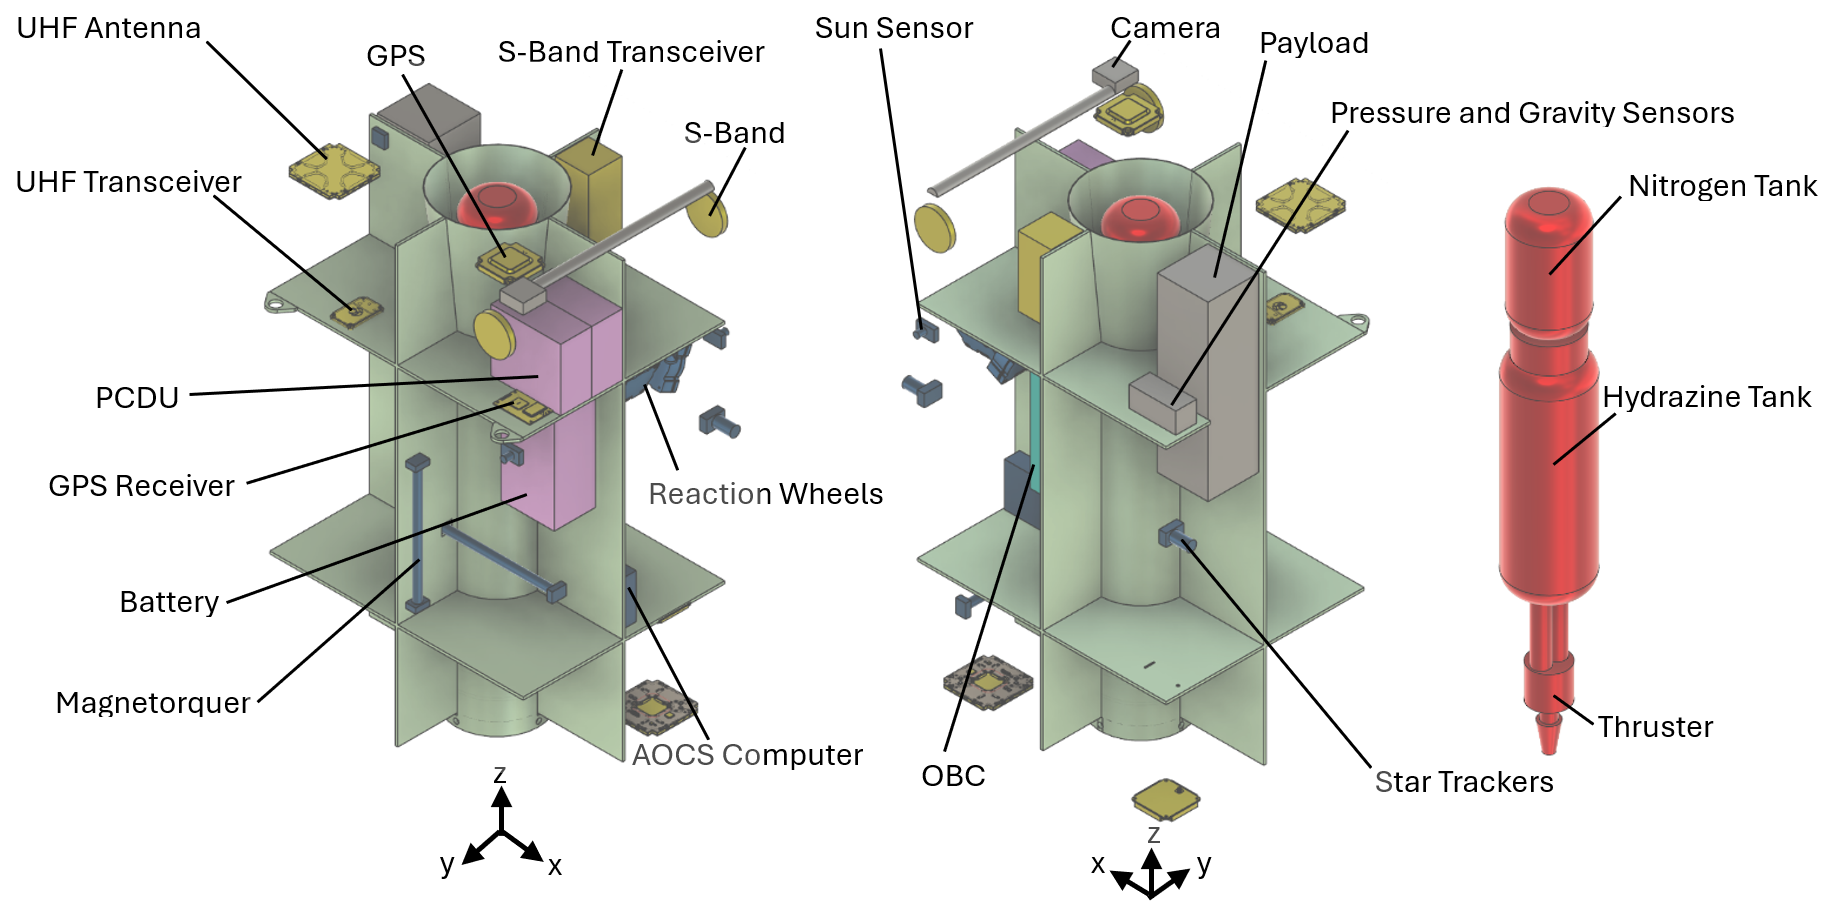
\includegraphics[width=0.8\linewidth]{figures/spacecraft_component_configuration.png}
    \caption{Configuration of Components}
    \label{fig:component_configuration}
\end{figure}

The outer configuration of SCIPIO-1 adopts a cuboid form-factor due to its strong flight heritage and simplicity \cite{StarfishSpace2024}. The shape also enables the use of body mounted solar panels and one-shot deployable panels which reduce mechanical complexity and risk. Two mounting points are also present, one for general satellite transport and AIT\label{nom:ait} (-Z face) and the other to enable rotation for attachment to the launcher interface (+Y face) complying with SFG-REQ-080 . Communication components, such as the UHF and S-Band antennas, and AOCS sensors are also mounted externally in pairs at opposite faces. This ensures consistent coverage of the required regions whilst the satellite is inertially fixed.

The primary driver for the internal component arrangement was the location of the Center of Gravity (CG) measured from the center of the interface ring. The distance of the CG in the X and Y axes is minimised to reduce the torque induced by the thruster. Meanwhile, the distance in the Z axis must be below 400mm to comply with Falcon 9 requirements (SAT-REQ-032). Heavy components have therefore been placed as close to the separation ring as possible. The reaction wheels are placed near the CG for improved control efficiency, with the magnetorquers separated to reduce electromagnetic interference. The position of the propulsion system within the central cylinder minimises thruster misalignment and ensures the CG is minimally affected as fuel level drops. Components are placed as close as possible within their respective subsystems to reduce harness lengths.

\subsection{Secondary Payloads}
In addition to Space Forge's CVD payload, SCIPIO-1 will support three secondary payloads to ensure objectives OBJ-02/03/04 are met. SFG-REQ-140 and SFG-REQ-160 demand microgravity and pressure sensors within 100\,mm of the primary payload, whilst SFG-REQ-230 necessitates a deployable marketing 'selfie' camera. The sensors were specifically chosen for high resolution at their low operating ranges. Low mass and power draw were favourable characteristics in the selection of all three secondary payloads.

For pressure sensing, the MKS 971B UniMag Cold Cathode Pressure Transducer was selected, as it was the only readily available sensor capable of measuring pressures low as $0.001\,\mathrm{mPa}$. Its implementation enables verification of SFG-REQ-170 on orbit, ensuring suitable payload operating conditions. Though it is rated for adverse environmental conditions, the sensor itself is not space-rated. As identified in Section~\ref{sub:risks}, this poses a significant developmental risk. For microgravity sensing, the Silicon Sensing CAS290 accelerometer was selected, due to its suitable precision and heritage use in a previous Space Forge mission \cite{noauthor_empowering_2024}. The Infinity Avionics LEO2MP camera was selected for the marketing camera; it similarly achieves TRL-9 status and is appropriately rated for the space environment. Addressing the field-of-view requirement, it will be mounted at the end of a $350\,\mathrm{mm}$ single shot deployable arm; the hold down spring release mechanism will be actuated by a burn-wire.

\label{sub:secondary_payloads}

\subsection{Structures}
\subsubsection{Concept Selection}
The structural design of the satellite has been driven by requirement SFG-REQ-030, to be compatible with the Falcon 9 launcher system. During the PDR phase, efforts were taken to also comply with SFG-REQ-040 and SFG-REQ-050 to ensure compatibility with the Electron and Arianne 6 launchers. However, due to Space Forge’s suggestion to choose one launcher, the design has been optimised for Falcon 9 loads, post-PDR. A compromise was made to have a cuboid form with internal central column and shear walls, to simplify configuration of internal components and external solar cell placement, as opposed to a circular monocoque construction. The configuration has proven heritage due to various past missions utilising similar structural design \cite{StarfishSpace2024}. Various materials were compared and Aluminium-6061-T6 was originally down selected for the structure due to being easy to manufacture with, cheap and having moderately high specific strength. Moreover, it possesses good thermal conductivity, potentially allowing thermal pathways to be formed as part of the structure, optimising on mass. However, after further investigation it was determined that this didn’t provide the required specific stiffness whilst adhering to the allocated mass budget, therefore CFRP was considered moving forward.
% Configuration is valid to put in structures bit here due to space of config section, but should be omitted in the tech report
% I dont know how to word the "this config.." till the end should be done, but it can definitely be shortened and made more concise
\subsubsection{Final Design}
A central cone that tapers to a constant diameter cylinder will act as the primary structure, due to efficiently transferring the launch loads from the launch ring to the rest of the satellite. To facilitate this, the larger diameter of the cone is matched to that of the separation ring. Four shear webs are attached to the column equidistant from each other, to transfer the shear loads to the outer walls, with external components such as the solar array and antennas mounted to the outer walls. Two shelves will be attached along the length of the column to provide mounting space for internal components, whilst acting as ribs to support the outer walls and improve torsional stiffness.

Hexcel IM7/8552 \cite{IM7/8552} was the CFRP of choice, which was down-selected for its high specific strength and stiffness properties. Moreover, it has low CTE, preventing heat loss during eclipse, and low magnetic interaction, reducing interference with the magnetorquers. Quasi-isotropic layups were used during analysis of the main structure due to their predictable performance. For the deployable solar array, a honeycomb sandwich panel was down-selected due to its very high specific stiffness, to help avoid resonance of a very large plate. Hexcel CR III 5052 ¼ inch cell size honeycomb core \cite{hexwebcr3} was chosen with Aluminium 6061-T6 \cite{Al-6061-T6} foil for the face to achieve this.

\begin{table}[h!]
\centering
\caption{Structural Component Analysis Results}
\label{tab:structural_analysis}
\begin{tabular}{@{}lccccc@{}}
\toprule
& \textbf{Central Column} & \textbf{Root Shear Webs} & \textbf{Mid + Tip Shear Webs} & \textbf{Outer Walls} & \textbf{Shelves} \\
\midrule
\textbf{Critical Loading} & Shear Stress & Shear Stress & Shear Buckling & Shear Buckling & Vibration \\
\midrule
\textbf{Reserve Factor} & 4.02 & 5.51 & 1.19 & 2.43 & 2.69 \\
\textbf{Mass (kg)} & 0.698 & 0.339 & 0.717 & 4.500 & 0.853 \\
\bottomrule
\end{tabular}
\end{table}

\subsection{Propulsion}
\subsubsection{Concept Selection}
To ensure that SCIPIO-1 represents a technological advance compared with Space Forge’s ForgeStar-1, the targeted deorbit of the satellite was deemed a crucial aspect of the mission. Initially, 3 possible methods of deorbit were identified: chemical propulsion, electrical propulsion, and a drag sail. This section briefly outlines these methods, and why chemical propulsion was ultimately selected.

Employed by ForgeStar-1, a drag sail simply increases the satellite’s drag in the upper atmosphere, eventually deorbiting the spacecraft. Although mission analysis tools like DRAMA and STK enable deorbit predictions, atmospheric uncertainties introduce variability in the landing ellipse, and thus reduce the degree of landing precision. An electrical propulsion system accelerates plasma through an electric field, providing very high ISP, but with insufficient force.  The retrograde burn of an electrical thruster similarly provides too small a force to guarantee landing within a target region. With SCIPIO-1’s non-compliance with the demisability requirement (SFG-REQ-110), it is paramount that the platform has sufficient thrust to ensure a landing in the SPOUA which solidified the choice of chemical propulsion.

\subsubsection{Final Design}
Within chemical propulsion, there exist monopropellant and bipropellant liquid designs. Choosing reduced mass and simplicity over a small gain in ISP, SCIPIO-1 employs a $5\,\mathrm{N}$ Hydrazine monopropellant thruster. A Rafael $5\,\mathrm{N}$ thruster was down-selected with an MCDA, see \autoref{tab:thrusterdownselection}, for its low mass and power draw, along an integrated valve, filter, and catalyst heating bed.

The Hydrazine bladder fuel tank is pressurised to $110\,\mathrm{bar}$ with gaseous Nitrogen, providing a constant ISP and thrust. The feed system has been designed with fault-tolerance and safety first, using requirements derived from the Falcon 9 rideshare user guide. The propellant release lines are fault-tolerant, using 2 latching solenoid valves actuated by separate electronic commands. There are 3 pressure transducers strategically placed within the system, monitoring tank pressures. Heritage was valued in the selection of all components.


\subsection{Attitude and Orbit Control System}
\subsubsection{Concept Selection}
The AOCS must satisfy several mission–level requirements: maintaining a microgravity environment at the payload (SFG-REQ-150), achieving on-board position and velocity knowledge (SFG-REQ-190), detumbling from $2^{\circ}\,\mathrm{s}^{-1}$ during LEOP (SFG-REQ-220), and tolerating thrust-vector errors during manoeuvres (AOC-REQ-001). With these drivers in mind, magnetorquer-only control for science mode and reaction wheels for high slew rates were chosen. 

A variety of different control actuation strategies were considered. Control Moment Gyros (CMGs) and reaction thrusters were ruled out due to their excessive mass, as well as complicated mechanisms. CMGs contain many moving parts, creating more single points of failure. Passive methods, on the other hand, cannot ensure active pointing ability and hence directly violate the inertial pointing requirement. Additionally, they may not counter unknown disturbances effectively, and are entirely unable to counter any torque generated by thruster misalignment. The analysis led to the selection of MTQs for nominal operation inertial pointing, and a set of four reaction wheels for all modes outside of science and safe. A further trade study is available in the appendix at \autoref{tab:actuator_downselection}.

\begin{table}[H]
\centering
\caption{Comparison of Control Actuation Options}
\begin{tabular}{p{3cm} p{7cm} p{7cm}}
\hline
 & \textbf{Capabilities} 
 & \textbf{Limitations} \\
\hline

\cellcolor{yellow!25}\textbf{MTQs} 
 & \cellcolor{yellow!25}Low disturbance and reliable actuation with enough control for detumble and nominal pointing 
 & \cellcolor{yellow!25}Insufficient torque for high slew manoeuvres \\ 
\hline

\cellcolor{yellow!25}\textbf{Reaction Wheels} 
 & \cellcolor{yellow!25}High torque and bandwidth with fast detumble and tight pointing 
 & \cellcolor{yellow!25}Excessive vibrations, high power draw, moving parts \\ 
\hline

\textbf{CMGs} 
 & Very high torque and fast manoeuvre capability 
 & Very heavy, moving parts, strong vibrations \\ 
\hline

\textbf{Passive Methods} 
 & Simple concepts that require no active hardware 
 & No active pointing and cannot counter misalignment torques \\ 
\hline

\textbf{Reaction Thrusters} 
 & High torque and strong control authority 
 & Highly complex and too heavy \\ 
\hline

\end{tabular}
\label{tab:actuators}
\end{table}

Sensor-suite depth was evaluated as well, from coarse sun–mag solutions to full star tracker grade knowledge. Coarse sun sensors and earth horizon sensors were deemed too low resolution to act as absolute sensors. All other sensors, including high FoV fine sun sensors, star trackers, magnetometers, IMU, and GNSS modules were considered critical to maintain compliance with Space Forge requirements. A further trade study is available in the appendix at \autoref{tab:sensor_downselection}.

\begin{table}[H]
\centering
\caption{Summary of Attitude Sensors}
\begin{tabular}{p{3cm} p{7cm} p{7cm}}
\hline
 & \textbf{Role} 
 & \textbf{Key Characteristics} \\
\hline
\cellcolor{yellow!25}\textbf{Star Tracker} 
 & \cellcolor{yellow!25}Primary attitude sensor during science, safe modes, inertial pointing, IMU calibration 
 & \cellcolor{yellow!25}High accuracy and low noise; requires clear star field; acquisition time; limited by slew rate \\ 
\hline
\cellcolor{yellow!25}\textbf{Fine Sun Sensor} 
 & \cellcolor{yellow!25}Primary attitude sensor in science, safe, and rapid data modes 
 & \cellcolor{yellow!25}Low power and reliable; only works when Sun is visible; coarse accuracy \\ 
\hline
\cellcolor{yellow!25}\textbf{Magnetometer} 
 & \cellcolor{yellow!25}Supports detumble and MTQ-based control 
 & \cellcolor{yellow!25}Measures local magnetic field; accuracy limited by magnetic cleanliness and onboard disturbances \\ 
\hline
\cellcolor{yellow!25}\textbf{Gyroscope / IMU} 
 & \cellcolor{yellow!25}High-rate propagation between absolute sensor updates 
 & \cellcolor{yellow!25}Good short-term stability; drifts over time; needs correction from star tracker or sun sensors \\ 
\hline
\cellcolor{yellow!25}\textbf{GNSS} 
 & \cellcolor{yellow!25}Provides position and velocity information 
 & \cellcolor{yellow!25}Useful for collision warnings and mission diagnostics \\ 
\hline
\textbf{Coarse Sun Sensor} 
 & Redundancy for sun sensors 
 & Resolution too low for attitude determination \\ 
\hline
\textbf{Earth Horizon Sensor} 
 & Supplemental attitude sensor 
 & Very low resolution and high noise \\ 
\hline
\end{tabular}
\label{tab:sensors}
\end{table}

%Coarse sun sensors and Earth horizon sensors were deemed too low resolution to act as redundancies and hence were excluded from the final design.


\subsubsection{Final Design}

The final attitude control configuration is based on the trade results in the previous section. 

\begin{table}[H]
\centering
\begin{minipage}[t]{0.47\textwidth}
\centering
\caption{Selected Sensors}
\begin{tabular}{l l l}
\hline
\textbf{Part} & \textbf{Supplier} & \textbf{Model} \\
\hline
2x High FOV Fine Sun Sensor & CubeSpace & CubeSense Sun \\
2x Star Tracker & CubeSpace & CubeStar \\
Magnetometer & CubeSpace & CubeMag Compact \\
GNSS Receiver & SkyFox Labs & piNAV-NG/FM \\
2x GNSS Antenna & SkyFox Labs & piPATCH-MAX/FM \\
\hline
\end{tabular}
\end{minipage}
\hfill
\begin{minipage}[t]{0.47\textwidth}
\centering
\caption{Selected Actuators}
\begin{tabular}{l l l}
\hline
\textbf{Part} & \textbf{Supplier} & \textbf{Model} \\
\hline
3x MTQ & CubeSpace & CR0100 \\
4x Reaction Wheel & CubeSpace & CW1200 \\
\hline
\end{tabular}
\end{minipage}
\end{table}



Expected disturbance torques of order $10^{-6}\,\mathrm{N\,m}$ are low enough for magnetorquer-based control during nominal operations. 
Three MTQs, rated at $10\,\mathrm{A\,m^2}$ each, provide all control authority in nominal operations, manage momentum unloading in other modes, and detumbling. High slew rate manoeuvres are handled by four reaction wheels in a tetrahedral configuration. Each wheel delivers up to $1.6\times10^{-2}\,\mathrm{N\,m}$, giving margin for slews and recovery from off-nominal attitudes. The four-wheel configuration has a probability of losing three axis control over 2 years of $\sim2.9\times10^{-6}$, which was a significantly reduced risk compared to the $2.1\times10^{-3}$ probability of the same event with three reaction wheels instead.

The chosen components' usage within each nominal operational mode is shown in \autoref{tab:aocs_modes}.

\begin{table}[H]
\centering
\caption{AOCS Component Usage Across Operational Modes}

\newcommand{\idle}{\ding{109}}   % open circle
\newcommand{\nom}{\ding{108}}    % filled circle
\newcommand{\peak}{\ding{115}}   % filled triangle

\begin{tabular}{l c c c c}
\hline
\textbf{Component} &
\textbf{Science Mode} &
\textbf{Safe Mode} &
\textbf{Collision Avoidance} &
\textbf{Rapid Data Transfer} \\
\hline
\multicolumn{5}{l}{\idle\ Idle \quad \nom\ Nominal \quad \peak\ Peak} \\
\hline

Payload 
& \nom\ \peak 
& \idle 
& \idle 
& \idle \\

Magnetorquers 
& \nom\ \peak 
& \nom\ \peak 
& \nom\ \peak 
& \nom\ \peak \\

Reaction Wheels 
& \idle/\nom 
& \idle/\nom 
& \nom\ \peak 
& \nom\ \peak \\

Star Trackers 
& \nom\ \peak 
& \idle\ \peak 
& \idle 
& \idle \\

Sun Sensors 
& \nom\ \peak 
& \nom\ \peak 
& \idle/\nom 
& \idle/\nom \\

Magnetometer 
& \nom\ \peak 
& \nom\ \peak 
& \nom\ \peak 
& \nom\ \peak \\

IMU 
& \nom\ \peak 
& \nom\ \peak 
& \nom\ \peak 
& \nom\ \peak \\

\hline
\end{tabular}\label{tab:aocs_modes}
\end{table}

\subsection{Communications and OBDH}
\subsubsection{Concept Selection}
SCIPIO-1 requires a consistent communication link to transmit platform and scientific data. To meet the differing cadence requirements and enhance communication resilience, data was separated into critical and bulk telemetry. To achieve this architecture, two separate frequencies were required: one for critical telemetry, which requires wide coverage and low attenuation properties to meet access time requirements, and one for bulk data requiring high data rates. For critical telemetry, it was a trade-off between two low frequencies, VHF and UHF, as they offer wide coverage experiencing lower attenuation. However, UHF was ultimately chosen because of its commercial availability for ground station communication. For bulk telemetry, both S-band and X-band frequencies are considered due to their wide usage in microsatellite missions. Although X-Band offers higher data rates, its directionality demands more precise pointing, which was not possible given the payload's inertial fixing requirement (SFG-REQ-320). X-band is also more susceptible to atmospheric attenuation, particularly rain fade, leading to reduced performance during adverse weather conditions. Therefore, S-band was selected for its moderate coverage and reliability. 




%After identifying  communication requirements, frequency bands were selected to meet downlink rate and access time requirements. The ground stations were then selected based on frequency capabilities as well as location, where northern ground stations were favourable due to SCIPIO-1’s highly inclined orbit. To select the communication components, group 4 prioritised factors such as: data sheet availability, heritage and volume. Radios were then selected based on frequency, data rates and transceiver power. Finally, the antennas were selected focusing on radio compatibility and antenna gain. 

To handle the data generated by the satellite, a capable On-board Computer (OBC) is required. Given the criticality of the component, fault tolerance was prioritised, whilst ensuring the required independent timekeeping features are present (SFG-REQ-210). The satellite's raw data generation, found using values from literature~\cite{wertz_space_1999}, was estimated at around $1.1\,\mathrm{GB}$ per day. This drove the sizing of the internal data storage.

\subsubsection{Final Design}
%(SFG-REQ-250, SFG-REQ-260, SFG-REQ-270, SFG-REQ-280, SFG-REQ-290, SFG-REQ-300,SFG-REQ-310, SFG-REQ-330).
%(SFG-REQ-250, SFG-REQ-260, SFG-REQ-270, , SFG-REQ-300, SFG-REQ-330).
The critical data is transmitted through UHF at a frequency of $400\,\mathrm{MHz}$ and a downlink rate of $38.6\,\mathrm{kbps}$. This uses GMSK modulation because of its high main-lobe to side-lobe suppression properties, resulting in low attenuation. Bulk telemetry is transmitted through a full duplex transceiver using two separate S-band frequencies, downlinking at $2.250\,\mathrm{GHz}$ and receiving at $2.075\,\mathrm{GHz}$ to minimize interference . The transceiver is programmed with BPSK modulation uplink as it is robust  modulation scheme and reduces interference. QPSK is used for downlink because high spectral efficiency as a result of its efficient bandwidth usage. The radios and antennas  for UHF and S-Band communication is shown in table \ref{tab:comm_comp} . Each UHF and S-Band system can receive the minimum  rate of 1 command per second (SFG-REQ-270), where S-Band transceiver is capable of full duplex communication (SFG-REQ-250)

The Terran network ground network was selected, primarily due its two high latitude UHF ground station stations to meet the 2 hour and 4 hour  critical cadence requirement (SFG-REQ-310) (SFG-REQ-290). Furthermore, addition of three S-Band ground stations allows for high data rate transfers for image down links (SFG-REQ-330), transmission of bulk platform data (SFG-REQ-280), bulk payload data (SFG-REQ-300)  and allows for real time telemetry (SFG-REQ-200). It also enables access times in excess of 5 minutes (SFG-REQ-260).
\begin{table}[H]
    \centering
    \caption{Communication subsystem components}
    \label{tab:comm_comp}
    % Define column layout: l for the Category column, c for centered data columns
    \begin{tabular}{l c c c c}
        \toprule
        % Header for Frequency Bands
        \textbf{Category} & \multicolumn{2}{c}{\textbf{UHF}} & \multicolumn{2}{c}{\textbf{S-band}} \\
        % Partial rules for subgrouping
        \midrule
        % Header for Component Type
        & \textbf{Antenna} & \textbf{Radio} & \textbf{Antenna} & \textbf{Radio} \\
        \midrule
        % Data Row: Component Model
        \textbf{Component Model} & 
            \begin{tabular}[t]{@{}l@{}}Small Antenna \\ Module (2)\end{tabular} & 
            Murgas radio (2) & 
            \begin{tabular}[t]{@{}l@{}}Anywaves TT\&C \\ S-band antenna (2)\end{tabular} & 
            \begin{tabular}[t]{@{}l@{}}Slink-Phy \\ SpaceCom (1)\end{tabular} \\
        \midrule
        % Data Row: Manufacturer
        \textbf{Manufacturer} & \multicolumn{2}{c}{Spacemanic} & Anywaves & SpaceCom \\
        \bottomrule
    \end{tabular}
\end{table}

The Cavu Johnston has been selected as the central onboard computer. Capable of independent time keeping (SFG-REQ-210), this model offers hot redundant voltage regulation and a built-in watchdog for system recovery. With $24\,\mathrm{GB}$ of Flash memory, it offers a generous data margin, allowing more than 20 days of raw data storage. Whilst this is potentially excessive, it significantly reduces the risk of data loss in the event of a prolonged communications outage. The incurred mass penalty was therefore deemed acceptable within the current design. Additionally, the presence of three storage partitions would significantly reduce the number of data erase cycles, thus mitigating against data storage degradation.

% Keep the design/budget discussion compact without stretching vertical gaps.
\begingroup
\raggedbottom
\setlength{\parskip}{4pt}
\edef\restoreFlowTopNumber{\arabic{topnumber}}
\edef\restoreFlowBottomNumber{\arabic{bottomnumber}}
\edef\restoreFlowTotalNumber{\arabic{totalnumber}}
\renewcommand{\topfraction}{0.9}
\renewcommand{\bottomfraction}{0.8}
\renewcommand{\textfraction}{0.1}
\renewcommand{\floatpagefraction}{0.75}
\setcounter{topnumber}{3}
\setcounter{bottomnumber}{2}
\setcounter{totalnumber}{5}
\subsection{Thermal}
\subsubsection{Concept Selection}
In order to keep the payload (PLT-REQ-072) and all other platform components (THM-REQ-011) within their safe temperature ranges, a range of components were considered, including heating and cooling solutions. To minimise heat absorption, low-absorptivity films will be applied to the satellite’s outer surface, particularly on sun facing faces. High-emissivity coatings were further chosen to dissipate excess heat, acting as radiators. Heat will be dispersed throughout the satellite’s body using heat pipes, chosen over thermal straps due to greater heritage. Thermofoil heaters, thermostatically controlled by thermistors near critical components, will provide heating. Fluid coolers and deployable radiatiors were omitted from the design due to their high complexity, especially given the hot case only exceeding maximum system temperature by $4^\circ\,\mathrm{C}$.
\subsubsection{Final Design}
The final configuration of the thermal subsystem, alongside each component’s contributions to it can be seen within \autoref{tab:thermal_control}. The coatings selected for the external surfaces not only contribute to keeping all components within their operational temperature ranges, but also protect it from atomic oxygen degradation due to a \ce{SiO2} coating. 

\begin{table}[!htbp]
\centering
\caption{Thermal Subsystem Architecture}
\label{tab:thermal_control}
\begin{tabular}{p{4.5cm}p{8.5cm}}
\toprule
\textbf{Component} & \textbf{Functionality} \\
\midrule
\ce{SiO2}-coated aluminised Kapton & Placed on all external faces not containing solar cells, provides a balanced absorptivity to emissivity ratio and protects against atomic oxygen degradation \\
\addlinespace
Silver-coated FEP & Placed on external faces containing solar cells, selected for their high emissivity to offset the solar cells' high absorptivity \\
\addlinespace
Heat Pipes & Used to distribute heat from components generating significant heat to those requiring heating/radiating surfaces \\
\addlinespace
Thermistors & Placed near key components, used as sensors for thermostatic control of heaters \\
\addlinespace
Polyimide Thermofoil Heaters & 8 etched foil heaters providing up to $160\,\mathrm{W}$ of heating to components whose operating temperature exceeds the cold case \\
\bottomrule
\end{tabular}
\end{table}

\subsection{Power}
\subsubsection{Concept Selection}
To meet the customer requirement of all power being generated from solar energy (SFG-REQ-240), solar photovoltaic cells were selected as the primary power source for the mission. A trade-off study (\autoref{tab:cellmcda}) was conducted to determine the technology best suitable for the component. This resulted in multijunction GaAs-based solar cells being selected over single junction GaAs and silicon cells due to their significantly higher efficiency being beneficial to the satellite’s small envelope. All thin-film cells were eliminated due to their low efficiency despite the potential for mass saving if used. The mission’s selected mid-morning SSO necessitated the inclusion of energy storage in the form of batteries as secondary power sources, due to the significant eclipse periods during each orbit preventing the solar cells from supplying power. Lithium-Ion cells were chosen due to their superior energy density reducing the mass needed, despite their lower cycle life relative to alternative nickel-based battery technologies (as seen in \autoref{tab:battery_mcda}). The combination of solar cells for generation and Li-Ion batteries for storage is a flight-proven one, supplying power to heritage platforms such as the Otterpup 2 \cite{StarfishSpace2024}.
\subsubsection{Final Design}
The parameters of the SA and battery are available within \autoref{tab:solar_array} and \autoref{tab:battery}. Cavu Aerospace triple junction GaAs-based SC-3GA-4 cells were selected for the mission for their high ($32\%$) efficiency, low radiation degradation, and availability, being manufactured by a British supplier. The cells were arranged into four sections: the main body-mounted array will generate power in all mission modes alongside two one-shot deployable arrays, while an additional smaller array on the opposite face of the satellite’s body will provide additional power in LEOP, Collision Avoidance, and Decommissioning modes. MP Space’s Pack2 8SP3 Li-Ion battery was selected to be the platform energy storage owing to its high energy density, wide window of operating temperatures, and a robust battery management system. The batteries were designed to operate at a DoD of no more than 30\% in nominal operations to mitigate the moderate cycle life of Li-Ion batteries. The power will be conditioned and distributed using a pair of Bradford Space SuperNova PCDUs, providing power to all subsystems via four voltage buses, including a nominal $28\,\mathrm{V}$ bus and three regulated rails of $3.3$, $5$, and $12\,\mathrm{V}$. The choice of two PCDUs was driven by the decision to eliminate all single points of failure within the power system due to all other subsystems’ reliance on it.


\begin{table}[!htbp]
\centering
\begin{minipage}{0.46\textwidth}
\centering
\caption{Solar Array Properties}
\label{tab:solar_array}
\begin{tabular}{@{}ll@{}}
\toprule
\textbf{Parameter} & \textbf{Value} \\
\midrule
No. of Cells & $312$ \\
\quad Facing +Y & $247$ \\
\quad Facing -Y & $70$ \\
Cell Efficiency & $32\%$ \\
Science Mode Power Demand (OAP) & $93\,\mathrm{W}$ \\
EOL Science Mode Power Generation (OAP) & $169.4\,\mathrm{W}$ \\
Main Array Configuration & 11s22p \\
Total Cell Area & $0.96\,\mathrm{m}^2$ \\
Total Cell Mass (incl. margin) & $0.79\,\mathrm{kg}$ \\
\bottomrule
\end{tabular}
\end{minipage}
\hfill
\begin{minipage}{0.46\textwidth}
\centering
\caption{Battery Properties}
\label{tab:battery}
\begin{tabular}{@{}ll@{}}
\toprule
\textbf{Parameter} & \textbf{Value} \\
\midrule
Capacity & $432\,\mathrm{W\,h}$ \\
Nominal Voltage & $28.8\,\mathrm{V}$ \\
Mass (incl. margin) & $2.45\,\mathrm{kg}$ \\
Design DoD & $30\%$ \\
Cell Architecture & 8s3p \\
\bottomrule
\end{tabular}
\end{minipage}
\end{table}
% ---------------------------------------------------------------------------
% 7. SYSTEM BUDGETS
% ---------------------------------------------------------------------------
\FloatBarrier
\section{System Budgets}
\subsection{Mass Budget}
A bottom-up component mass budget was created, with margins applied to each component according to heritage, as per the ESA margin philosophy \cite{noauthor_sre-pa2011097_2012}. The harness mass has been estimated at 5\% of satellite dry mass, using the same ESA Standard. The subsystem mass breakdowns are included in Table~\ref{tab:mass_budget} below, each rounded off to the nearest $100\,\mathrm{g}$. 
\begin{table}[!htbp]
\caption{Subsystem mass budget}
\label{tab:mass_budget}
%\normalsize
\centering
\begin{tabular}{l c}
\toprule
\textbf{Subsystem} & \textbf{Mass with Margin ($\mathrm{kg}$)} \\
\midrule
Comms/OBDH              & $1.6$ \\
Thermal                 & $1.2$ \\
Power                   & $5.3$ \\
Payload                 & $4.1$ \\
AOCS                    & $4.0$ \\
Propulsion              & $8.0$ \\
Harnessing              & $1.6$ \\
Structure               & $12.2$ \\
\midrule
Total Dry Mass (kg)     & $38.0$ \\
\midrule
Propellant              & $3.0$ \\
\midrule
Total Wet Mass (kg)     & $41.0$ \\
\bottomrule
\end{tabular}
\end{table}

Although the spacecraft wet mass is below the upper limit dictated by SFG-REQ-060, it is nearing it. As detailed in \autoref{sec:crit_anal}, there are ways to reduce the satellite mass. Full  mass budget is detailed in the Appendix, \autoref{tab:Final_Verif_Plan}.

\subsection{$\Delta V$ Budget}\label{sub:deltav}
The $\Delta V$ budget was prepared by combining the worst case deorbit scenario with a conservative 12 collision avoidance scenarios per year. The deorbit values were found via ESA's DRAMA software, then verified using STK's Astrogator, as detailed in Section~\ref{sub:Miss_Anal_TR}. The $\Delta V$ for collision avoidance was found using this approximate form of Hohmann transfers for small changes in orbit altitude $ \Delta V \approx 0.5\left(\frac{\Delta r}{r}\right)V_{A/B}$. It was taken from SMAD~\cite{wertz_space_1999}; a $100\,\mathrm{m}$ change in altitude was considered.

\begin{table}[!htbp]
\centering
\caption{Mission Delta-V Requirements}
\label{tab:deltaV}
\begin{tabular}{lccc}
\toprule
\textbf{Manoeuvre Type} & \textbf{Delta-V ($\mathrm{m\,s}^{-1}$)} & \textbf{Propellant Mass ($\mathrm{kg}$)} & \textbf{Propellant Volume ($\mathrm{L}$)} \\
\midrule
Collision Avoidance & $1.98$ & $0.04$ & $0.039$\\
Deorbit & $130.51$ & $2.38$ & $2.33$ \\
Total without Margin & $132.49$ & $2.41$ & $2.36$\\
\midrule
Total with Margin (10\%) & $145.74$ & $2.66$ & $2.61$\\
\bottomrule
\end{tabular}
\end{table}

\subsection{Power Budget}
The power budget applies the same ESA margin philosophy \cite{noauthor_sre-pa2011097_2012} utilised by the mass budget. A $5\%$ EOL degradation margin was applied to all post-Commissioning modes, with a further $5\%$ transmission loss applied, as prescribed by the PCDU data sheet. Power generation values were obtained using worst-case sun angles generated over a year using STK. The primary arrays will generate power in all modes, with the secondary arrays providing additional power in LEOP, Collision Avoidance, Deorbit, and Decommissioning. Power expenditure was determined using a bottom-up approach, determining the duty cycles of each component over the duration of an orbit. 
\begin{table}[!htbp]
\centering
\caption{Power Budget by Mission Mode}
\label{tab:power_budget}
\begin{tabular}{lccc}
\toprule
\textbf{Mode} & \textbf{OAP Generation [$\mathrm{W}$]} & \textbf{OAP Expenditure [$\mathrm{W}$]} & \textbf{Balance [$\mathrm{W}$]} \\
\midrule
LEOP & $138.5$ & $135.6$ & $2.8$ \\
Commissioning & $178.3$ & $121.3$ & $57.0$ \\
Science Mode & $169.4$ & $93.0$ & $76.4$ \\
Safe Mode & $182.7$ & $79.0$ & $103.7$ \\
Collision Avoidance & $86.5$ & $155.0$ & $-68.5$ \\
Deorbit Burn & $86.5$ & $223.0$ & $-136.6$ \\
Decommissioning & $86.5$ & $149.1$ & $-62.6$ \\
\bottomrule
\end{tabular}
\end{table}

\subsection{Thermal Limits}

The thermal limits of all components were obtained by consulting the manufacturer's data sheets. Due to the propulsion system only being operational during Deorbit and transient Collision Avoidance, its Operational thermal limits have not been taken into account for the overall platform.

\begin{table}[!htbp]
\centering
\caption{Temperature Limits for Components}
\label{tab:temperature}
\begin{tabular}{l
    >{\raggedleft\arraybackslash}p{2.2cm}
    >{\raggedleft\arraybackslash}p{2.2cm}
    >{\raggedleft\arraybackslash}p{2.2cm}
    >{\raggedleft\arraybackslash}p{2.2cm}}
\toprule
\textbf{Component} & 
\textbf{Min Operational T [$^\circ\,\mathrm{C}$]} & 
\textbf{Max Operational T [$^\circ\,\mathrm{C}$]} & 
\textbf{Min Non-operational T [$^\circ\,\mathrm{C}$]} & 
\textbf{Max Non-operational T [$^\circ\,\mathrm{C}$]} \\
\midrule
Gravity Sensor & $-40$ & $125$ & & \\
Camera & $-20$ & $60$ & & \\
Space Forge Payload & $-35$ & $85$ & & \\
Pressure Sensor & $0$ & $40$ & & \\
Thruster & $4$ & $90$ & $-10$ & $90$ \\
Propellant Tank & $10$ & $50$ & $-5$ & $65$ \\
Pressure Regulator & $-53$ & $66$ & & \\
Latching Valve & $5$ & $80$ & $-10$ & $90$ \\
UHF Transceiver & $-40$ & $85$ & & \\
UHF Antenna & $-40$ & $85$ & & \\
S Transceiver & $-20$ & $50$ & & \\
S Antenna & $-120$ & $120$ & & \\
GPS Receiver & $-40$ & $85$ & & \\
OBC & $-40$ & $85$ & & \\
AOCS Sensors & $-35$ & $80$ & & \\
AOCS Actuators & $-35$ & $80$ & & \\
Battery & & & & \\
\quad Charge: & $0$ & $55$ & & \\
\quad Discharge: & $-30$ & $55$ & & \\
PCDUs & $-30$ & $60$ & & \\
\midrule
\textbf{SYSTEM TOTAL} & \textbf{5} & \textbf{40} & \textbf{-5} & \textbf{65} \\
\bottomrule
\end{tabular}
\end{table}

\subsection{Link Budget}
\autoref{tab:linkbudget_clean} outlines the communication system assumptions and the respective link margins for both UHF and S-band communications. A separate RDT mode column has been included for S-band as this involves transmission at a higher data rate. All margins exceed recommended 6dB needed for near Earth communicationsdB~\cite{wertz_space_1999}. The summary of the assumed losses is included in~\autoref{sub:comms_obdh_TR}, with the full link budget included in~\autoref{tab:fedr_link_budget}.


\begin{table}[!htbp]
    \centering
    \caption{Link Budget Properties}
    \label{tab:linkbudget_clean}
    % Define column layout: l for the Variable column, c for centered data columns
    \begin{tabular}{l c c c c c c}
        \toprule
        % Header Level 1: Downlink and Uplink
        \textbf{Variable} & \multicolumn{3}{c}{\textbf{Downlink}} & \multicolumn{3}{c}{\textbf{Uplink}} \\
        \midrule
        % Header Level 2: Frequency Band and Function combined
        % UHF Critical | S-Band Nominal | S-Band RDT | UHF Critical | S-Band Nominal | S-Band RDT
        & \textbf{UHF} & \multicolumn{2}{c}{\textbf{S-Band}} & \textbf{UHF} & \multicolumn{2}{c}{\textbf{S-Band}} \\
        \midrule
        & \textbf{Critical} & \textbf{Nominal} & \textbf{RDT} & \textbf{Critical} & \textbf{Nominal} & \textbf{RDT} \\
        \midrule
        % Data Rows
        Function & Critical & Nominal & RDT & Critical & Nominal & RDT \\
        Frequency (GHz) & 0.400 & 2.250 & 2.250 & 0.400 & 2.075 & 2.075 \\
        Distance to ground (km) & 3000 & 3000 & 2000 & 3000 & 3000 & 2000 \\
        Rate (kbps) & 38.6 & 600 & 4000 & 9.6 & 64.0 & 64.0 \\
        Modulation & GMSK & QPSK & QPSK & GMSK & BPSK & BPSK \\
        \midrule
        % Link Margin Row (Bold)
        \textbf{Link Margin (dB)} & \textbf{11.1} & \textbf{6.5} & \textbf{6.3} & \textbf{17.2} & \textbf{10.2} & \textbf{18.2} \\
        \bottomrule
    \end{tabular}
\end{table}
\subsection{Data Budget}

\autoref{tab:data_budget_main} below summarises the data downlink budget. A full description of the data budget is included within~\autoref{sub:comms_obdh_TR}, with the full budget included in Appendix~\ref{sub:FULL_DATA_BUDGET}. In all cases, the daily downlink potential exceeds the estimated generation. Rapid data transfer mode offers significant downlink potential, enabling the transfer of over 24 hours of bulk telemetry in a single pass.

\begin{table}[!htbp]
    \centering
    \caption{Data Budget}
    \label{sub:data_budget}
    \label{tab:data_budget_main}
    \begin{tabular}{l c c c}
        \toprule
        \textbf{Properties} & \multicolumn{3}{c}{\textbf{Frequency Band}} \\
        \midrule
        % Header for the Frequency Bands, spanned over the operational modes
        & \textbf{UHF} & \multicolumn{2}{c}{\textbf{S-Band}} \\
        \midrule
        \multicolumn{4}{l}{\textbf{Downlink}} \\ % Section Header for Downlink
        \midrule
        Function & Critical & Nominal & RDT \\
        Transceiver Data Rate (kbps) & 38.6 & 600 & 4000 \\
        Effective Data Rate (kbps) & 24.4 & 380 & 2530 \\
        Average Access Time Per 24 hours (s) & 1640 & 3770 & 4580 \\
        Data Volume Per 24 hours (MB) & 50.1 & 179 & 1450 \\
        \midrule
        \multicolumn{4}{l}{\textbf{Generation}} \\ % Section Header for Generation
        \midrule
        Data Type & Critical & \multicolumn{2}{c}{Bulk} \\ % Bulk spans Nominal and RDT columns
        Platform Generation (MB/24hrs) & 28.3 & \multicolumn{2}{c}{51.1} \\
        Payload Generation (MB/24hrs) & Neg & \multicolumn{2}{c}{11.1} \\
        Total Generation (MB/24hrs) & 28.3 & \multicolumn{2}{c}{62.2} \\
        \midrule
        \textbf{Margin (MB)} & \textbf{21.8} & \textbf{116.8} & \textbf{1387.8} \\
        \bottomrule
    \end{tabular}
\end{table}
% ---------------------------------------------------------------------------
% 8. TECHNOLOGY LEVELS AND RISKS
% ---------------------------------------------------------------------------
\FloatBarrier
\section{Technology Levels and Risks}
\label{sub:risks}
\subsection{Technology Readiness Levels}


Though efforts have been made to utilise heritage, Commercial Off-The-Shelf (COTS) components where possible, a selection of components fall short of this, and thus pose additional developmental risk. The highest risk component at present is the selected Cold Cathode Vacuum Transducer, introduced in Section~\ref{sub:secondary_payloads}. The use of this component was deemed a necessary risk, as it achieves the sub-millipascal precision necessary to verify SFG-REQ-170 on orbit. No space-rated alternative could be sourced which achieves comparable precision. In order to use such a component in space, it will require a full qualification testing regime, including thermal vacuum (TVAC\label{nom:tvac}), vibration, shock and radiation testing. The sensor is fabricated from inherently low-outgassing materials, like stainless steel and titanium, though more specific material specifications would be needed to confirm compliance with ECSS-Q-ST-70-02C~\cite{ECSS-Q-ST-70-02C_2008}. A test campaign like this would undoubtedly incur a cost penalty for the customer and delay the mission timeline. 

Several components utilised within the design are space-qualified, but have no flight-heritage, and are thus assessed as TRL-8\label{nom:trl}. One such component is the MP Space Li-ion Battery Pack~\cite{MPSpacePack2_2024}, which is scheduled to obtain heritage in 2026. In addition to this, though the CubeADCS suite has flight heritage, they do not disclose component-specific heritage status. In the absence of explicit confirmation, these components are conservatively treated as non-heritage, and appropriate design margins have been applied. Beyond technical risk, some components also introduce programmatic risk. The composite overwrapped pressurant tank - chosen for its US DOT certification - is supplied by L3Harris, an American defense contractor. This will likely mean that the tank is subject to ITAR restrictions, complicating procurement.

\subsection{Risk Identification and Assessment}
As shown in the product breakdown structure in Appendix~\ref{sub:scipio_pbs}, the power, OBDH, AOCS and propulsion systems have been identified as critical subsystems, meaning they pose significant technical risk, and drive mission success. A Failure Modes and Effects Analysis (FMEA\label{nom:fmea}) was utilised during the project to evaluate component failure modes, and the risk they pose. For each of the critical subsystems, the failure mode with the highest Risk Priority Numbers (RPN\label{nom:rpn}) is summarised below in Table~\ref{tab:fmea}.

\begin{table}[!htbp]
    \centering
    \caption{Failure Modes and Effects Analysis (FMEA)}
    \renewcommand{\arraystretch}{1.3}

    % Effect = 0.8X, Cause = 0.8X, Mitigation = 1.4X
    \begin{tabularx}{\linewidth}{
        l
        >{\hsize=.8\hsize\relax}X
        >{\hsize=.8\hsize\relax}X
        c
        >{\hsize=1.4\hsize\relax}X
    }
        \toprule
        \textbf{Failure Mode} &
        \textbf{Effect} &
        \textbf{Cause} &
        \textbf{RPN} &
        \textbf{Mitigation} \\
        \midrule

        PCDU Failure &
        Loss of power to all subsystems &
        Shorts, overheating, internal wiring faults &
        $240$ &
        Hot-redundant PCDU implemented to ensure continuous spacecraft operation in the event of a failure. \\

        OBC Failure &
        Satellite unable to send, receive, or process commands &
        SEUs, software errors, ESD damage, radiation-induced latch-up, electrical faults &
        $240$ &
        OBC rated for $30\,\mathrm{krad}$ TID; redundant voltage regulation; built-in watchdog functionality. \\

        Thruster Failure &
        Loss of control during firing, posing collision risk to nearby spacecraft &
        Clogged valves, nozzle damage from launch loads, thermal cycling &
        $324$ &
        Avoidance of non-critical manoeuvres; heritage propulsion hardware; redundant valves and pressure transducers. \\

        Reaction Wheel Saturation &
        Loss of attitude control during manoeuvres, posing collision risk to nearby spacecraft &
        Momentum Accumulation during deorbit burn, due to thruster misalignment &
        $360$ &
        No current measures - deorbit burn will have to be segmented into multiple shorter 2 minute burns, to allow magnetorquers to desaturate the wheels.\\

        Incomplete Burn-up &
        Ground Casualty Risk Introduced; Increased Regulatory Challenges &
        Use of high melting point components, like COPVs and the CFRP structure. &
        $300$ &
        Controlled, targeted re-entry into the SPOUA.\\
        
        \bottomrule
    \end{tabularx}
    \label{tab:fmea}
\end{table}
Evidently, loss of power is appropriately mitigated by the implementation of a redundant PCDU. This, combined with the power system's tolerance to a single solar panel deployment failure, and dual battery string failures, make it a robust subsystem design. The same cannot be said for the OBC which remains a major single point-of-failure within the design. Though a fault tolerant OBC has been selected, introduction of a redundant OBC would considerably reduce failure risk. 

The saturation of the reaction wheels currently represents one of the most significant mission risks in the current design iteration. Though the wheels were sized to counteract thruster misalignment torque, the accumulation of momentum was not accounted for during initial subsystem design, and has since been discovered to be a certainty. Fortunately, discovery at this stage means the failure can be mitigated by design. The mitigations for this failure mode are detailed in Section~\ref{sub:ThrusterMomentum}.

Loss of control due to thruster failure has also been identified as a significant mission-level failure mode, particularly combined with the satellite’s incomplete demise. Although the risk of incomplete burn-up is partially mitigated by selecting a remote re-entry corridor, successful targeting is entirely dependent on thruster capability. As such, the re-entry footprint would become unpredictable, substantially increasing ground casualty risk, and potentially violating deorbit regulations. By enhancing the satellite's demisability, this risk would be significantly reduced, as detailed in Section~\ref{sub:demisability}
% ---------------------------------------------------------------------------
% 9. REQUIREMENTS COMPLIANCE
% ---------------------------------------------------------------------------
\FloatBarrier
\section{Requirements Compliance}

In accordance with ECSS-E-ST-10-02C \cite{noauthor_ecss-e-st-10-02c_2018}, the requirements were sorted into one of the four standard  verification types. At this stage in the project, only ``Review of Design" (D) and ``Analysis" (A) verification is possible, with ``Inspection" (I) and ``Testing" (T) reserved for post-AIT mission phases. Table~\ref{tab:critical_VM} below shows the current verification status for each of the ``critical" customer requirements, with the full customer and derived verification matrices contained within Appendix~\ref{subsec:reqs_verif_appendix}. It should be noted that full verification of all requirements is not possible within the scope of this project and as such, these tables indicate preliminary compliance. A table of the planned, final verification activities is therefore also included in Appendix~\ref{subsec:reqs_verif_appendix}.
\begin{table}[!htbp]
\centering
\caption{Verification Matrix for ``Critical" Customer Requirements}
\begin{tabularx}{\textwidth}{l c c X}
\toprule
\textbf{Req. ID} & \textbf{Compliance} & \textbf{Type} & \textbf{Evidence}\\
\midrule
SFG-REQ-010 & Yes & \textbf{A} & Compliance is predicted based on balanced budgets, mission lifetime analysis and extensive use of heritage components.\\
SFG-REQ-030 & Yes & \textbf{D/A} & All derived launch vehicle compatibility requirements for Falcon 9 have been met (XXX-REQ-031 to XXX-REQ-039). \\
SFG-REQ-070 & Yes & \textbf{D/A} & All payload accommodation requirements have been met (including the derived requirements XXX-REQ-071 to XXX-REQ-077), ensuring the necessary electrical, mechanical and communications provisions are made, and environmental conditions are suitable for operation. \\
SFG-REQ-140 & Yes & \textbf{D} & Inspection of the CAD shows the microgravity sensor within $100\,\mathrm{mm}$ of the payload. \\
SFG-REQ-150 & Yes & \textbf{A} & AOCS simulations show that magnetorquers are capable of maintaining payload accelerations below $10^{-4}\,\mathrm{g}$ during payload operations. \\
SFG-REQ-160 & Yes & \textbf{D} & Inspection of the CAD shows the pressure sensor within $100\mathrm{mm}$ of the payload. \\
SFG-REQ-170 & Yes & \textbf{A} & Pressure does not exceed 1\,mPa throughout the mission lifetime, even in worst-case conditions (separation at lower tolerance limit, ECSS ``High" Solar and Geomagnetic Activity)\\
SFG-REQ-220 & Yes & \textbf{A} & AOCS simulations show detumbling within 3 minutes using reaction wheels.\\
SFG-REQ-230 & Yes & \textbf{D} & Inspection of CAD shows the camera is mounted to include the Earth and Satellite within the FOV \\
SFG-REQ-240 & Yes & \textbf{A} & Power budget shows margin in most modes, with batteries sized to handle the eclipse periods and deorbit burn. \\
SFG-REQ-270 & Yes & \textbf{D} & The UHF transceiver is capable of receiving $9600\,\mathrm{Bps}$, whilst the S-band transceiver can receive $64\,\mathrm{kBps}$ thus both are capable of receiving 1 payload telecommand per second. \\
SFG-REQ-290 & Yes & \textbf{A} & STK access analysis shows a maximum gap between passes of $84.6$ minutes over UHF using the Terran Network \\
SFG-REQ-300 & Yes & \textbf{A} & The data budget shows that daily downlink potential exceeds data generation per day. \\
SFG-REQ-310 & Yes & \textbf{A} & STK analysis shows a maximum gap between passes of $84.6$ minutes over UHF using the Terran Network. Data budget shows downlink potential exceeds size of critical TM packet \\
SFG-REQ-320 & Yes & \textbf{D} & Satellite is equipped with star trackers to enable inertial pointing in Science Mode. \\
SFG-REQ-350 & Yes & \textbf{D} & Inspection of CAD shows payload with its Y-face exposed \\

\bottomrule
\end{tabularx}
\label{tab:critical_VM}
\end{table}

Whilst all critical requirements have been met, several non-compliances remain in the current design iteration. The most significant is SFG-REQ-110, which regards the demisability of the satellite. Although plans to deorbit in the SPOUA mitigate the ground risk, it nevertheless introduces additional challenges in demonstrating regulatory compliance and obtaining the necessary licensing. Future design iterations should therefore seek to improve demisability. Another area in which SCIPIO-1 does not strictly comply with the customer's requirements is the Ariane 6 compatibility requirement, SFG-REQ-040. Though the satellite is volume compatible and can withstand load the test load cases, the structure's natural frequency is too low to be compatible with the launcher. Though further optimisation of the structure to be compatible with all three launchers would maximise flexibility, feedback from Space Forge during the PDR\label{nom:pdr} suggested that ruling out at least one of the launchers was expected. 





% ---------------------------------------------------------------------------
% 10. CRITICAL DESIGN ANALYSIS
% ---------------------------------------------------------------------------
\FloatBarrier
\section{Critical Design Analysis}\label{sec:crit_anal}

Whilst the current design iteration of SCIPIO-1 demonstrates strong progress toward a viable flight configuration, the accelerated timeline of the project has limited the opportunity for full design maturity. The following critical design analysis highlights the key shortcomings of the current design and the recommended improvements for subsequent iterations.

\subsection{Structural Optimisation}
FEA analysis indicates RFs above one for the modes currently considered, complying with SFG-REQ-030. However, this analysis only considers a purely composite layup. Exploring a combination of different materials for the main structure such as aluminium sandwich outer panels may optimise the design by increasing its specific stiffness and therefore, the natural frequency. This will help to comply with SFG-REQ-030/040/050. Furthermore, a reduction in the outer panel mass concentrates the satellite's mass towards the CG. This reduces torsional loads during launch and improves AOCS efficiency throughout the mission. Aluminium outer panels could also help to improve the demisability of the satellite, due to its lower melting point to composites. With design maturity, a more refined FEA model can be created allowing optimisation of the structural design.

\subsection{Demisability}
\label{sub:demisability}

One of the key shortcomings of the current SCIPIO-1 design iteration is its incomplete burn-up upon re-entry. As well as posing a ground casualty risk, this will introduce considerable programmatic delays, as additional regulatory approvals would be required. Although the transition to aluminium sandwich panels would enhance the demisability of the satellite, preliminary DRAMA analysis has found that the composite-overwrapped pressurant tank would still survive re-entry. However, the mass savings achievable through structural redesign would facilitate the transition to a heavier, but fully demisable aluminium pressure vessel. This change would not only ensure compliance with SFG-REQ-110, it would also address the identified procurement risk associated with ITAR-controlled components. The demisability of the propulsion system as a whole could be further improved by locating it outside the central load bearing cylinder. Though this would adversely impact the mass distribution of the satellite, it would promote the early release of and therefore the ultimate demise of the subsystem.

\subsection{Thruster Momentum Management}
\label{sub:ThrusterMomentum}
%-Reaction wheel saturation was not considered during propulsive manoeuvres.
%-Reaction wheels would saturate after ~2 mins, so burns could not be longer than this.
%-Mitigate by including dual thrusters, capable of differential thrust. This eliminates the need for the AOCS to perform the torque rejection. This also provides redundancy.
As identified in~\autoref{sub:risks}, the saturation of the reaction wheels during thruster operation poses a significant risk in the current design. Though the AOCS actuators were sized to counteract thruster misalignment torques, the resulting momentum accumulation was not considered. It has since been found that burns longer than 2 minutes will saturate the wheels, resulting in a loss of control during manoeuvres. This both poses a conjunction risk to nearby satellites and will render targeted re-entry impossible. Given the satellite's incomplete demise, this would likely mean the satellite cannot obtain the necessary launch licenses. Though the reaction wheels could be sized up for greater momentum storage, the optimal way to mitigate this would be to implement a symmetric dual thruster configuration. This would enable differential thrust, effectively eliminating the demand on the reaction wheels. Although it would add up to $1\,\mathrm{kg}$ to the satellite's mass, the potential mass savings from structural optimisations would facilitate this. Implementation of a secondary thruster would also introduce redundancy, improving the fault tolerance of the system.
\subsection{Single Points of Failure}
%-OBC, Thruster, Pressure Regulator, S-band Transceiver
Several single points of failure (SPOF) in multiple subsystems have been identified in the lead-up to the FDR. Firstly, although the selected OBC incorporates many redundancies within its architecture, its failure would be catastrophic to the mission as no commands could be processed anymore. Recent missions of similar envelope, such as the RISESat \cite{RISESat_eoportal_2024} have implemented a redundant processing unit, which could be considered for future design iterations. Similarly, since only one S-band transceiver is present within the platform, the data throughput would be significantly decreased in case of failure. Although the UHF Transceivers would be able to provide functional redundancy, including a formal redundancy within the S-band communications could be an option worth exploring in the future. Lastly, the propulsion system contains two SPOFs: the thruster and the pressure regulator. Although the selected orbit would allow natural deorbit within the prescribed timeline, a propulsion failure deem collision avoidance manoeuvres unachievable and a fully targeted re-entry impossible. Redundancies within satellites’ propulsion systems are commonplace, with missions such as VENuS \cite{Venus_eoportal} incorporating them within the design, and as such should be considered in the future. Though it adds substantial mass, an easy addition to the propulsion system would be a second pressure regulator in series providing redundancy.

\subsection{Thermal Management}
%-Current modelling is too coarse to give any accurate idea of component temperatures.
The transient lumped mass model used to approximate the thermal behaviour of the satellite was a moderate improvement over the static hot and cold case investigation, enabling the modelling of heat exchange using the properties of the thermal system’s components. However, it still offers a mere approximation of the temperature variation and does not factor in the distribution or dynamic duty cycles of internal heat sources. Thus, the thermal subsystem has likely been overdesigned, particularly regarding the implementation of heaters. Although unlikely to be required, up to $160\,\mathrm{W}$ of heating was allocated to the platform to mitigate against prolonged cold-case exposure. The design of the thermal system could be significantly improved using a multi-nodal model, allowing for the inclusion of individual components’ properties within the analysis, better optimising the subsystem for the conditions experienced by the platform. A higher fidelity model would also facilitate the implementation of thermal straps and heat pipes into the design; these have been identified as necessary for effective heat distribution around the satellite, but have not yet been designed in detail.  

% ---------------------------------------------------------------------------
% 11. WAYS OF WORKING
% ---------------------------------------------------------------------------
\section{Ways of Working}
% Team processes, tools, communication, lessons learned, etc.
The team adopted a working model derived from the concurrent engineering (CE) approach. With the project’s short timeline necessitating high intensity of operations, this was deemed to be the most efficient approach. The initial (pre-PDR) period was used to ensure that all team members familiarise themselves with the full scope of the project, with the subsequent phases of the project consisting of parallel efforts from each subsystem leads interlaced with frequent meetings focusing on progress and any issues blocking it. All resources were kept within an organised central repository available to all team members, making access to necessary information seamless. Those were used consistently throughout the project’s duration to allow iterative changes to the design, being able to immediately test any assumptions and feed the results back to the relevant team members. A central Gantt chart was used to monitor the top-level timeline of the project and proactively prevent any delays in the process, while a Kanban board created on Miro was used to track the actual completion stages for tasks assigned to each team member and compare them with the planned schedule. Being available to everyone, it also created an accountability mechanism preventing long periods of inactivity. Finally, during more complex phases of the project, work breakdown structures were created to assist in dividing large tasks into more manageable phases. 

% ---------------------------------------------------------------------------
% 12. SUMMARY
% ---------------------------------------------------------------------------
\section{Summary}

SCIPIO-1 represents a robust, pragmatic solution to Space Forge’s mission objectives. By utilising a $520\,\mathrm{km}$, 10:30 LTAN sun-synchronous orbit, the platform is able to provide the necessary low-pressure environment for payload operation, whilst the AOCS maintains the payload comfortably within the defined microgravity limits. A heritage-led subsystem design approach minimises technical risk, simplifies system integration, and accelerates the mission timeline. The power budget closes with a margin in nominal modes, with batteries sized to handle power-intensive periods. The same can be said of the link and data budgets, which support the verification of the mission's data-handling requirements. At the End of Life, SCIPIO-1 will perform a targeted re-entry into the SPOUA, to ensure fulfilment of Space Forge's deorbit objective. 

Whilst the current iteration is nearing design maturity, several key shortcomings require attention. The current platform does not fully demise during deorbit, with the satellite's pressurant tank surviving re-entry. This should be mitigated by reducing composite usage within the spacecraft, and instead shifting to more demisable aluminium alternatives. The use of aluminium honeycomb sandwich panels would also help optimise the structural mass and could enable Ariane~6 compatibility, by raising the satellite's natural frequency. Implementation of a secondary thruster would enable differential thrust, thus mitigating reaction saturation during firing. Several single points of failure have also been identified within the current design, which could be mitigated through targeted redundancy. Furthermore, the current thermal analysis lacks the fidelity required for detailed thermal design. Transitioning from a lumped mass model to a multi-nodal model will enable more accurate prediction of component temperatures and support more targeted thermal management. 
\FloatBarrier
\clearpage
\setcounter{topnumber}{\restoreFlowTopNumber}
\setcounter{bottomnumber}{\restoreFlowBottomNumber}
\setcounter{totalnumber}{\restoreFlowTotalNumber}
\endgroup


% ---------------------------------------------------------------------------
% 13. TECHNICAL REPORTS
% ---------------------------------------------------------------------------
\begin{titlepage}

	\vspace*{8mm}

	\begin{center}
		\rule[0.5ex]{\linewidth}{2pt}\vspace*{-\baselineskip}\vspace*{3.2pt}
		\rule[0.5ex]{\linewidth}{1pt}\\[\baselineskip]
		{\LARGE {AVDASI 2025 Space Group 4 Final Engineering Design Report}}\\[4mm]
        {\Large{Technical Reports}}\\[4mm]
		{\Large \textit{SS4 – SerenSpace}}\\
		\rule[0.5ex]{\linewidth}{1pt}\vspace*{-\baselineskip}\vspace{4.2pt}
		\rule[0.5ex]{\linewidth}{2pt}\\

		\vspace{6.5mm}
		{\large Authors: \\
			\textsc{Alan Wawrzyńczok\\
            Arnav Jabulee\\
            Asher Kapinos\\
            Nick Balboa\\
            Novanda Bardia Wahid\\
            Oliver Lee\\
            Romuald Saithanyan Christy Ruban}}\\

		\vspace{6.5mm}
		{\large Supervisors: \\
			\textsc{Dr. Yusuf Açar}\\
            \textsc{Ragnar Birgisson}}

		\vspace{4mm}
        
\includegraphics[height=80pt]{figures/university_of_bristol_crest}\hspace{30pt}%
        
\includegraphics[height=80pt]{figures/scipio1_mission_patch.png}

		\vspace{6mm}
		{\large \textit{School of Civil, Aerospace and Design Engineering}\\
			\vspace{6mm}
			\textsc{University of Bristol}}\\
		\vspace{6mm}
		\begin{minipage}{11.2cm}

			A report submitted to the University of Bristol in accordance with the requirements of the degree of \textsc{Master of Engineering} in Aerospace Engineering, as part of the \textsc{AVDASI 4 AENGM0060} module.
		\end{minipage}\\
		\vspace{11mm}
		{\large\textsc{December 2025}}
		\vspace{3mm}
	\end{center}

	%\begin{center}
		%\rule[0.5ex]{0.8\linewidth}{1pt}\vspace*{-\baselineskip}
		%\begin{tcolorbox}[standard jigsaw, opacityback=0,opacityframe = 0, coltitle=black, boxrule=0.5mm, arc=5mm, width=0.83\textwidth, bottom=2mm, left=2mm, right=2mm]
			%\begin{center}\textbf{Generative AI Declaration:\\[1em]}\end{center}
			%During the preparation of this coursework the student used OpenAI's CHATGPT to condense some sections for better page flow. After using this tool, the student reviewed and edited the content as needed and takes full responsibility for the content submitted for assessment.
		%\end{tcolorbox}
		%\vspace{-15pt}
		%\rule[0.5ex]{0.8\linewidth}{1pt}\vspace*{-\baselineskip}
	%\end{center}
	\vspace{2mm}


\end{titlepage}
\section{Technical Reports}
\subsection{Mission Analysis}
\label{sub:Miss_Anal_TR}
\subsubsection{Orbit Selection}

Table~\ref{tab:orbit_criteria} summarises the criteria considered in the initial orbit down-selection, the relevant driving requirements, and the preliminary assessment methodology. 

\begin{table}[H]
    \centering
    \caption{Orbit Down-selection Criteria}
    \renewcommand{\arraystretch}{1.2} % optional: increase row height
    \begin{tabularx}{\textwidth}{
        l
        >{\hsize=0.61\hsize}X
        >{\hsize=1.39\hsize}X
    }
        \toprule
        \textbf{Criteria} & \textbf{Applicable Requirements} & \textbf{Preliminary Assessment Technique}\\
        \midrule
        Power Generation & SFG-REQ-240, PLP-REQ-073, PLP-REQ-074, PLP-REQ-075 & Assessed using eclipse times from STK\\
        Communications Coverage & SFG-REQ-260, SFG-REQ-290, SFG-REQ-310 & Assessed using STK access data for candidate ground stations\\
        Thermal Stability & THM-REQ-011, PLT-REQ-072 & Assessed using eclipse times from STK\\
        Environmental Perturbations & SFG-REQ-150 & Assessed using Atmospheric Drag, Centrifugal and Gravity Gradient acceleration equations from SMAD\label{nom:smad} \cite{wertz_space_1999}\\
        Deorbit Lifetime & SFG-REQ-090, MIS-REQ-039 & Assessed using STK's Lifetime Tool and DRAMA's OSCAR Tool \\
        Radiation Dose & SFG-REQ-120, SFG-REQ-130 & Assessed using STK's SEET\label{nom:seet_stk} module \\
        Pressure & SFG-REQ-170 & Assessed using NRLMSISE 2.0~\cite{noauthor_nrlmsis_2025} Atmospheric Model\\
        Accessibility & SFG-REQ-030, SFG-REQ-040, SFG-REQ-050 & Assessed using launch vehicle user guides\\
        \bottomrule
    \end{tabularx}
    \label{tab:orbit_criteria}
\end{table}

Given the criticality of the pressure requirement, the pressure criterion posed more of a constraint than a driver. The exact altitude constraint was characterised using the NRLMSISE\label{nom:nrlmsise} 2.0 atmospheric model \cite{noauthor_nrlmsis_2025} and the ideal gas law.  Figure~\ref{fig:alt_plot} below shows the variation in pressure with altitude, at a range of standard solar activities \cite{noauthor_ecss-e-st-10-04c_nodate}. Evidently, the pressure is comfortably within the required limits over the typical LEO\label{nom:leo} altitude range, and as such, it could largely be neglected in orbit down-selection.

As described in Section 4.2, the FCC's deorbit requirement (MIS-REQ-032) was one of the primary constraints in altitude selection, whilst power generation, communication coverage and environmental perturbations all drove increasing altitude. Deorbit analysis was performed using both STK's Lifetime tool and DRAMA's OSCAR tool over a range of altitudes to determine an optimal altitude selection - this is depicted by the red circle in Figure~\ref{fig:deorbit_lifetime}. Note that the lifetime limit is set at 7 years, as this includes the 2 year mission lifetime. 

\noindent
\begin{minipage}{0.48\textwidth}
    \centering
    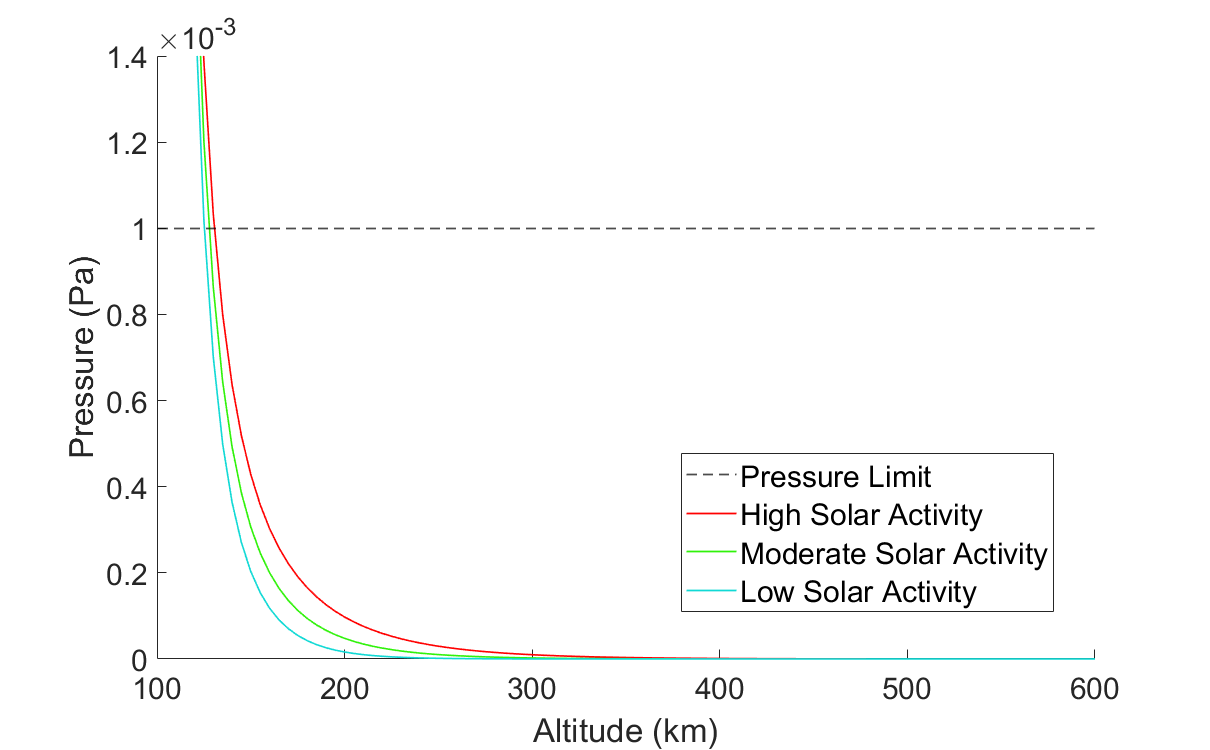
\includegraphics[width=\linewidth]{figures/atmospheric_pressure_vs_altitude.png}
    \captionof{figure}{Variation in Atmospheric Pressure with Altitude}
    \label{fig:alt_plot}
\end{minipage}
\begin{minipage}{0.48\textwidth}
    \centering
    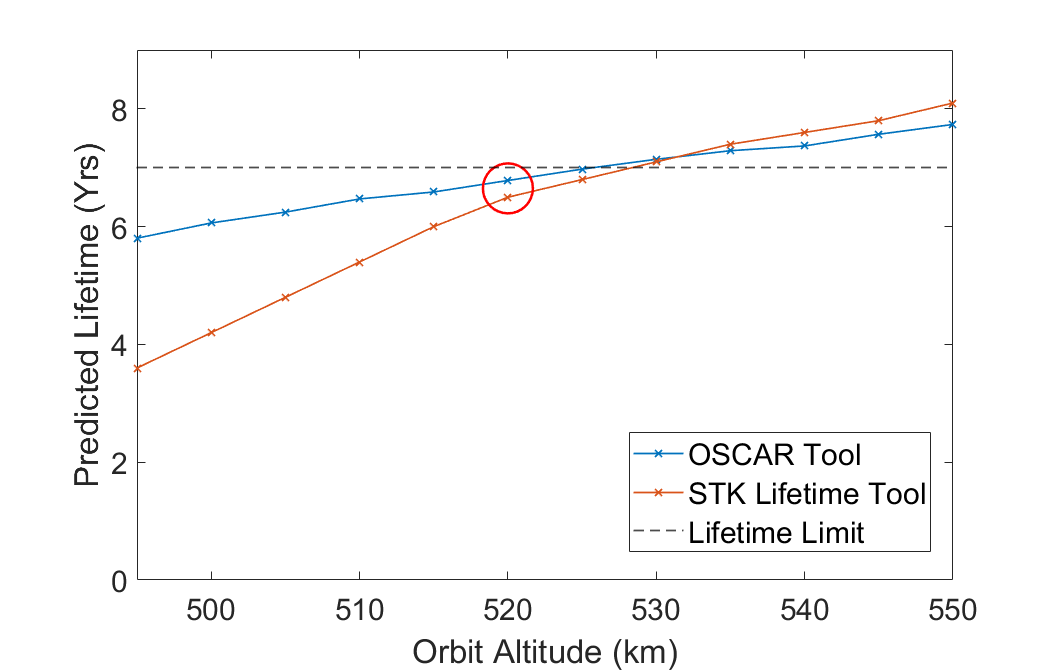
\includegraphics[width=\linewidth]{figures/deorbit_lifetime_vs_altitude.png}
    \captionof{figure}{Variation in Deorbit Lifetime with Altitude}
    \label{fig:deorbit_lifetime}
\end{minipage}\hfill

\subsubsection{Orbit Analysis}

With the orbit parameters in Table~\ref{tab:Orbit_Params} down-selected, verification of the 25-year dead-on-release deorbit requirement (SFG-REQ-090) was then necessary. To account for random tumble associated with a dead-on-release scenario, the mean projected area of the satellite was utilised, with the assumption of stowed solar panels. Using DRAMA's OSCAR tool, it was found that the deorbit life would lie between $6.3$ and $8.0$ years, with a $50\%$ confidence interval.\begin{figure}[H]
\centering 

To aid with verification of other subsystem level requirements, a range of other mission analyses were carried out. As detailed in Section~\ref{sub:comms_obdh_TR}, access analysis was performed to calculate data downlink potential. Furthermore, to more accurately predict power generation, the angular variation between the sun and solar panel vectors was also plotted - this is shown below in Figure~\ref{fig:solar_panel_angles}. The maxima, which correspond with the solstices, were used to give a worst-case power generation estimate.

%\hfill
\vspace{-10pt}
\centering
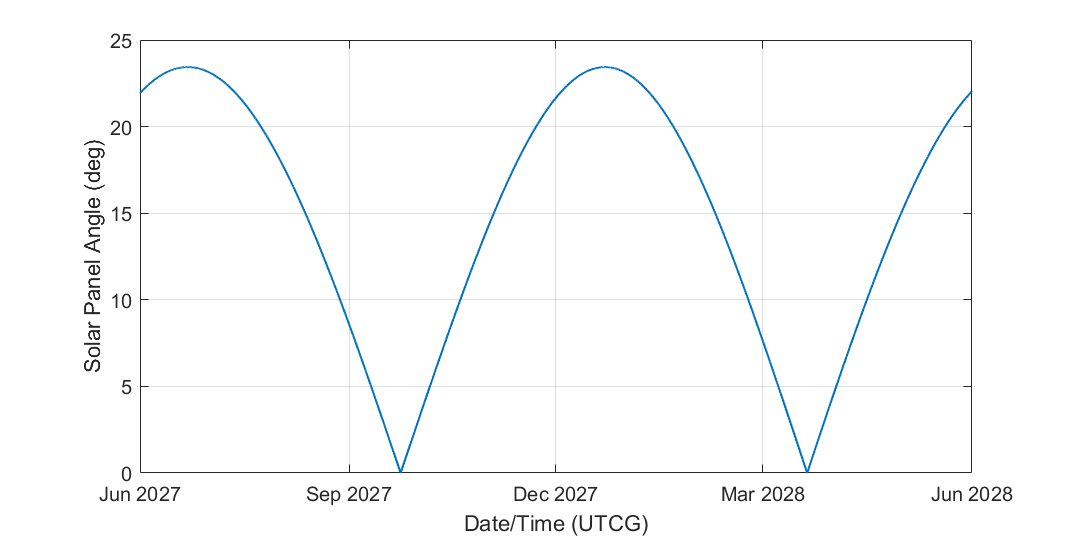
\includegraphics[width=0.65\linewidth]{figures/solar_panel_sun_angle_annual.png}
\captionof{figure}{Solar Panel Sun Angle Variation over 1 Year}
\label{fig:solar_panel_angles}

\end{figure}

\subsubsection{End of Life}

Although payload recovery would better align with Space Forge's long-term goals, preliminary research found that recovery systems for $40\,\mathrm{kg}$ microsatellites remain relatively novel \cite{cassell_adept_2018} \cite{sannino_re-entry_2025}, and hence introduce considerable risk. This, combined with the increased launch mass and regulatory requirements, informed the decision to perform a destructive re-entry. To plan the manoeuvre, a worst-case scenario was assumed, with an upper tolerance limit separation and a constant ``low" solar activity \cite{noauthor_ecss-e-st-10-04c_nodate}. The satellite was propagated for 2 years using a High Precision Orbit Propagator (HPOP\label{nom:hpop}), and the orbital parameters at the final epoch input into DRAMA's OSCAR\label{nom:oscar} tool. This estimated a delta-V of $130.5\,\mathrm{m\,s}^{-1}$ for direct re-entry.

As outlined in the AVDASI\label{nom:avdasi} 4 MRD\label{nom:mrd}, a strategic target re-entry region must be identified, to ensure the mission can act as a precursor for future missions. Initially, a subsection of the Icelandic BIRD FIR\label{nom:fir} was selected due to its strategic location near Space Forge's headquarters in the UK, as well as its proximity to Space Infrastructure at SaxaVord. Live ADS-B\label{nom:adsb} \cite{flightradar24_live_nodate} and AIS\label{nom:ais} \cite{noauthor_ship_nodate} data indicated that the region experienced relatively low air and shipping traffic, though more robust data would need to be obtained to confirm this. However, this re-entry region had to be changed after demisability analysis revealed that the satellite's would not burn up completely on re-entry - see Figure~\ref{fig:demise}.


The South Pacific Oceanic Uninhabited Area was therefore selected due to its remoteness, low flight and shipping activity, and its extensive heritage with satellite re-entry \cite{ESA_reentry_2017}. To plan the deorbit manoeuvre in STK, an Astrogator target sequence was defined in which the satellite propagates to a target Longitude of the Ascending Node (LAN\label{nom:lan}) before timing a finite $130.5\,\mathrm{m\,s}^{-1}$ burn to re-enter in the target region. A burn time of just over 19 minutes was recorded, indicated by the red line in Figure~\ref{fig:SPOUA_GT}. The final orbital parameters were then input into DRAMA's SARA tool to recompute the ground casualty risk. A coarse, 50-sample Monte Carlo Analysis was performed, varying both semi-major axis and true anomaly, which found that all samples were below the $10^{-4}\,\mathrm{g}$ casualty risk defined in ESSB-ST-U-007 \cite{ESA_reentry_2023}. Whilst this is indicative that the risk is mitigated, a much more extensive Monte Carlo analysis would be required to give confidence in the predicted re-entry footprint.

\begin{figure}[H]
    \centering
    \begin{minipage}{0.48\textwidth}
        \centering
        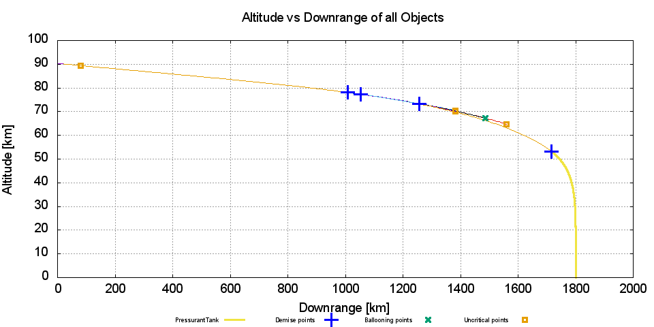
\includegraphics[width=\linewidth]{figures/spacecraft_demisability_analysis.png}
        \caption{SCIPIO-1 demisability analysis - the composite overwrapped pressurant tank survives re-entry}
        \label{fig:demise}
    \end{minipage}\hfill
    \begin{minipage}{0.48\textwidth}
        \centering
        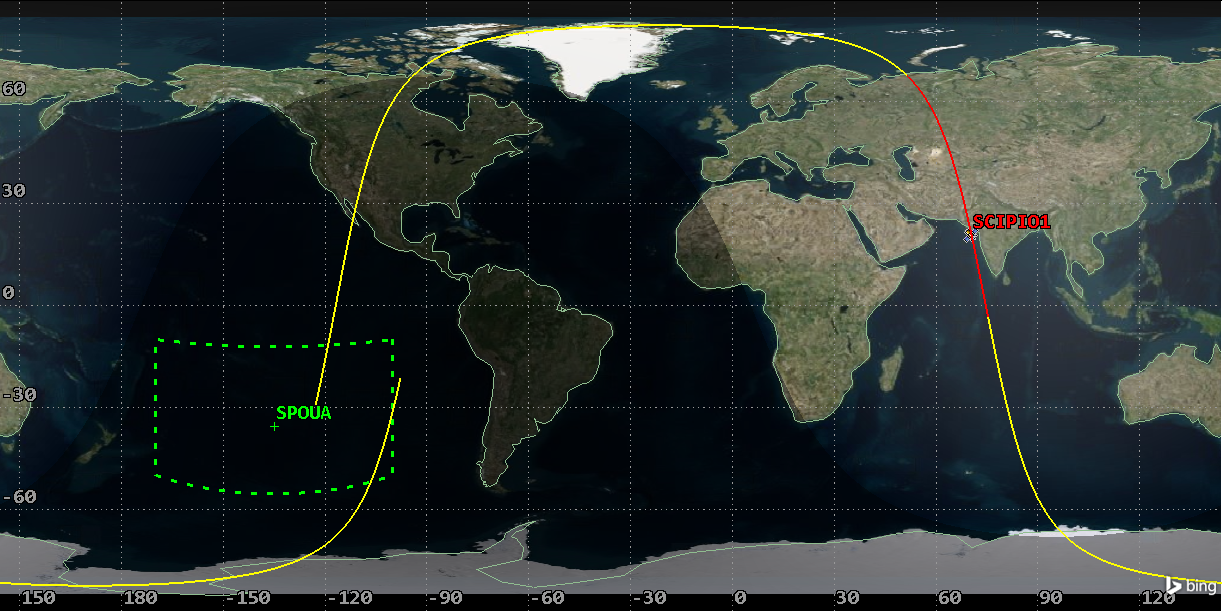
\includegraphics[width=\linewidth]{figures/deorbit_manoeuvre_ground_track.png}
        \caption{Deorbit manoeuvre ground track, with the finite burn indicated in red.}
        \label{fig:SPOUA_GT}
    \end{minipage}
\end{figure}


\subsection{Configuration}
The configuration of SCIPIO-1 is designed to accomodate all subsystem requirements. The initial design decision was to define the volume of the satellite. Space Forge sets and upper limit of $1200\times700\times700\,\mathrm{mm}$ (SFG-REQ-020). However, this would mean choosing large launcher envelopes that drives up the launch cost considerably. So, the decision was made to further limit the satellite main body volume to $850\times500\times400\,\mathrm{mm}$ to fit within the Falcon 9 quarter-plate envelope. This decision was reinforced by a heritage satellite the Otterpup 2 \cite{StarfishSpace2024}, which has similar mass and volume values. Although SCIPIO is optimised for Falcon 9 launcher requirements \cite{noauthor_falcon9rideshare_2024}, the satellite is also compatible with the volume envelopes of Ariane 62's 1/2 Hub and the Shared Electron fairing as in \autoref{fig:envelopes}. The chosen separation ring is also compatible across all platforms.
\begin{figure}[H]
    \centering
    \begin{minipage}{0.5\textwidth}
    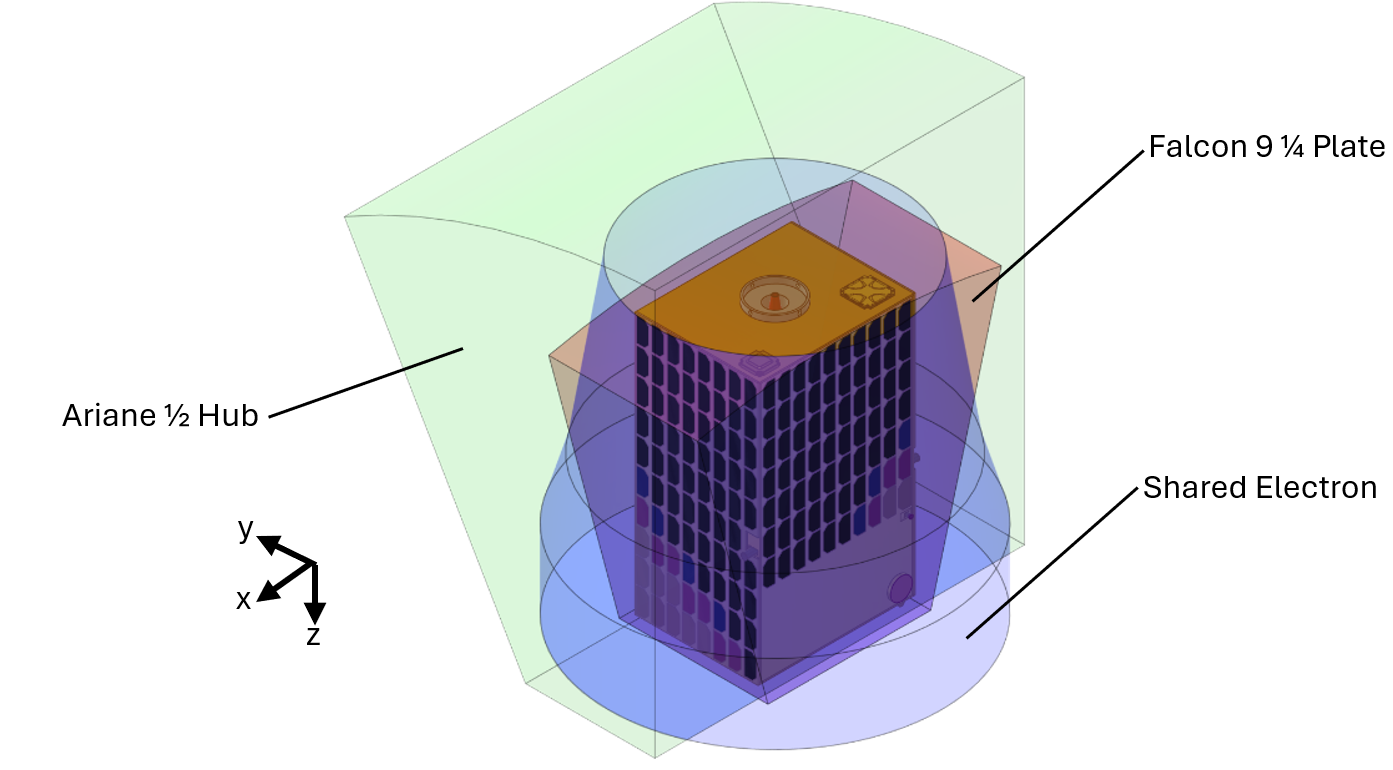
\includegraphics[width=1\linewidth]{figures/launcher_volume_envelopes.png}
    \caption{Volume envelopes of all 3 launchers}
    \label{fig:envelopes}

    \end{minipage}\hfill
    \begin{minipage}{0.5\textwidth}

    \centering
    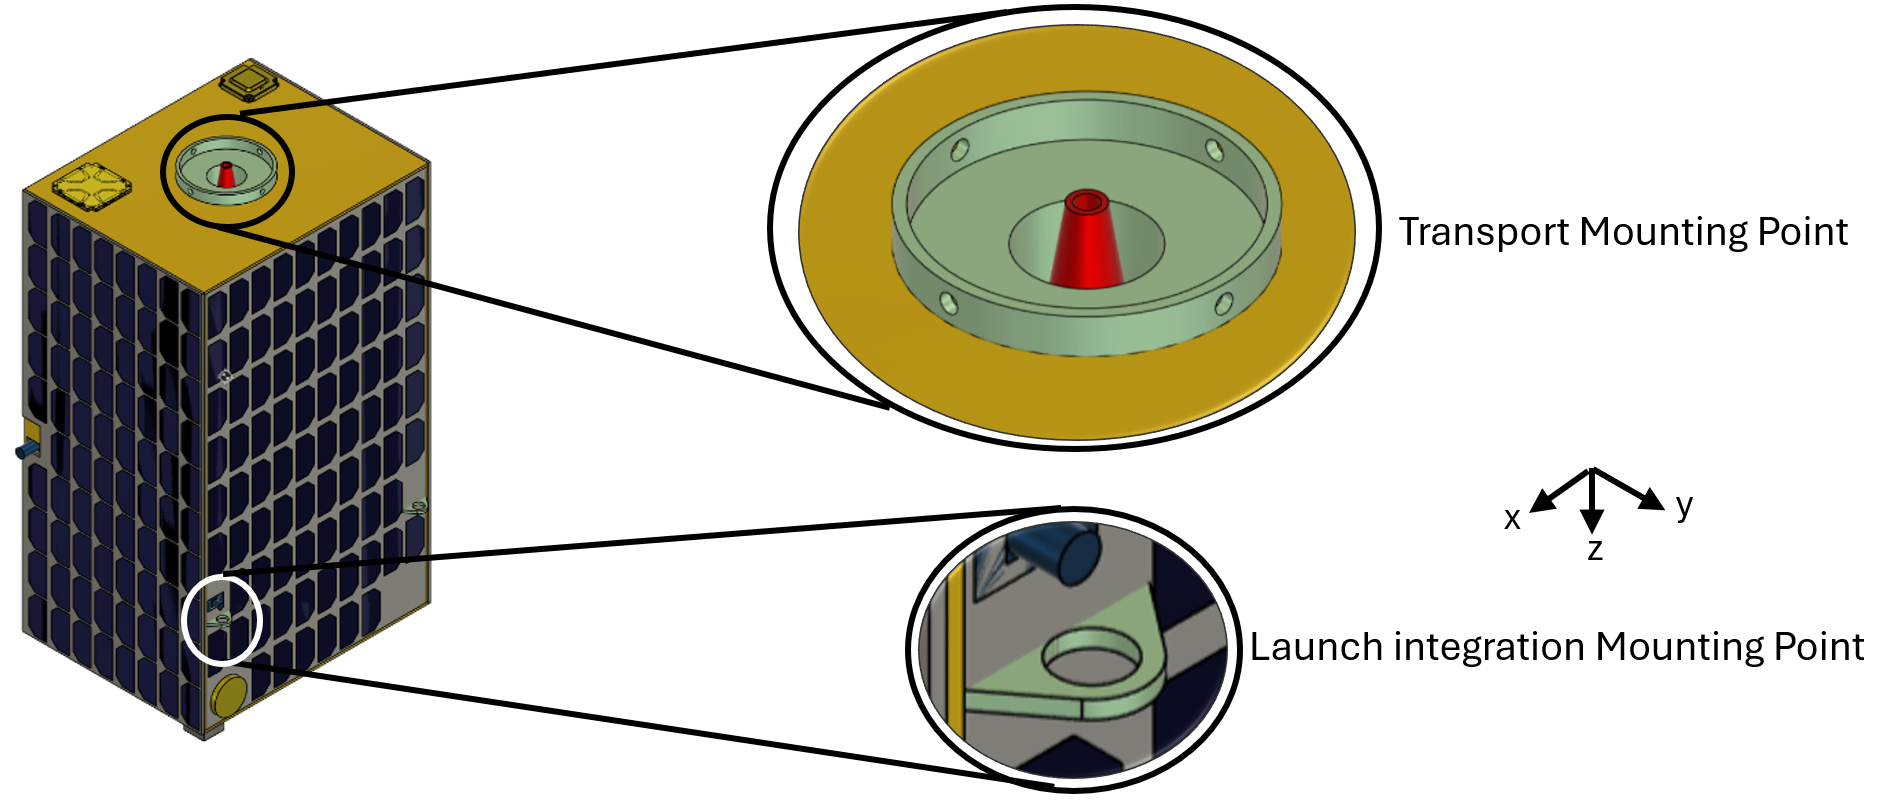
\includegraphics[width=1\linewidth]{figures/spacecraft_mounting_points.png}
    \caption{Mounting Points}
    \label{fig:mountings}
    \end{minipage}
\end{figure}

The focus of the structural design was load path optimisation. A central load-bearing cylindrical column was implemented, with diameter equal to that of the separation ring for effective load transfer. A taper was introduced at one end to maximise the usable volume within the satellite. Mounting points have been placed in line with the central cylinder to ensure ground handling loads can be effectively sustained. Two additional mounting points are included on the +Y face for launch integration, shown in \autoref{fig:mountings}. Four shear webs in each quadrant supports the main structure, while two shelves are placed for component mounting. Both shelves and webs also help maintain the natural frequency above launcher requirements. The cuboid outer body simplifies external component mounting and facilitates effective body-mounted solar panels.


The external power design features a primary body-mounted solar panel on the +Y face, supplemented by two one-shot deployable panels on the +/-X faces. When deployed, these will offer significant power generation potential, particularly while sun pointing in safe mode. A smaller, body-mounted array is included on the -Y face to maximise power generation during detumbling. All internal power components are placed next to each other, and as close to the body mounted solar panels to reduce cable lengths and power loss. 



For the AOCS, the four reaction wheels are placed as close to the CG to avoid unwanted translations and minimise structural wobbling The three magnetorquers each placed along their respective axes are futher away from the CG and spaced apart for increased torque and reduced electromagnetic interference respectively. To enable inertial pointing (SFG-REQ-320), two star trackers have been implemented internally on the +Y and -Y faces, with holes for external viewing. This placement ensures the sun is outside of the star tracker's sun-exclusion zone during nominal operations, whilst also enabling a constant view of the star field as in \autoref{fig:FOV}. Sun sensors on the +/-Y faces help with the detumbling process during LEOP and also attitude control to maximise power generation during safe and science mode.

\begin{figure}[H]
    \centering
    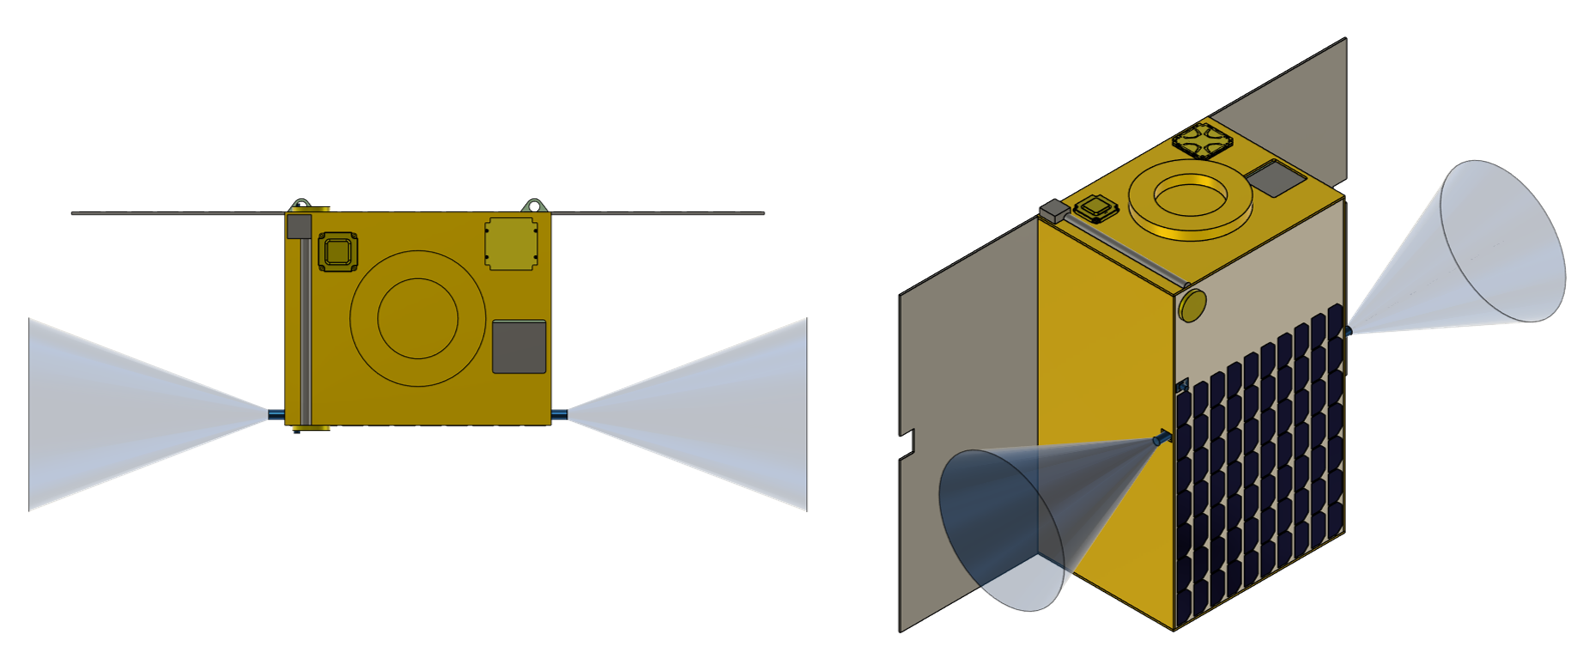
\includegraphics[width=0.7\linewidth]{figures/star_tracker_field_of_view.png}
    \caption{Star Tracker Field of View}
    \label{fig:FOV}
\end{figure}


The UHF antennas are located at the Z+/- to maximise access time with the high latitude ground stations and for communcation during detumbling. The S-band antennas are loacted at on Y+/- faces to communicate with the low latidue ground stations and accomodate the interial fixing requirements. Internally the trancievers are located close to the resepective antennas to reduce transmission loss. These are all connected to a central OBC that is also in the same compartment as the AOCS computer. This is to reduce attenuation losses and energy transfer.


The entire propulsion system is mounted within the central column. This ensures that the entire system is along the centre of gravity, thus minimising torques due to thruster misalignment. 

\subsection{Structures}

The structure was designed to satisfy requirement SFG-REQ-030, ensuring compatibility with the Falcon 9 launcher, with a breakdown of it available in \autoref{structuresexploded}. According to the ride-share guide \cite{noauthor_falcon9rideshare_2024}, the most demanding load case is the $16\,\mathrm{g}$ lateral and $4.5\,\mathrm{g}$ axial quasi-static acceleration loads, with an addition of $1.5\,\mathrm{g}$ lateral and $1.4\,\mathrm{g}$ axial due to sine loading. A safety factor of 2 has been used on all the loads, in accordance with guidance from SMAD \cite{wertz_space_1999}. Moreover, there is a minimum natural frequency limit of $40\mathrm{Hz}$ and a deflection margin of $10\,\mathrm{mm}$, due to the excess volume within the Falcon 9 ¼ plate.

\subsubsection{Material and Laminate Selection}

Preliminary analysis revealed that an Aluminium-6061-T6 structure does not provide the required specific stiffness within the allocated mass budget. Therefore, the entire satellite structure (excluding the deployable solar panels) uses CFRP IM7/8552 \cite{IM7/8552} unidirectional tape, with a Quasi-isotropic layup. Symmetric Quasi-isotropic layups lead to more predictable performance, reduce warping during manufacture, and avoid unexpected failures occasionally found in anisotropic layups from secondary loads. Honeycomb sandwich panels are used for the deployable solar array backing material. This provides the required specific stiffness to prevent resonance with the launcher adhering to the mass budget. Preliminary calculations determined that Hexcel CR III \sfrac{1}{4} inch cell size honeycomb core \cite{hexwebcr3} with Aluminium-6061-T6 \cite{Al-6061-T6} foil for the faces were sufficient. 


\subsubsection{Structural Configuration}

\begin{figure}[H]
    \centering
    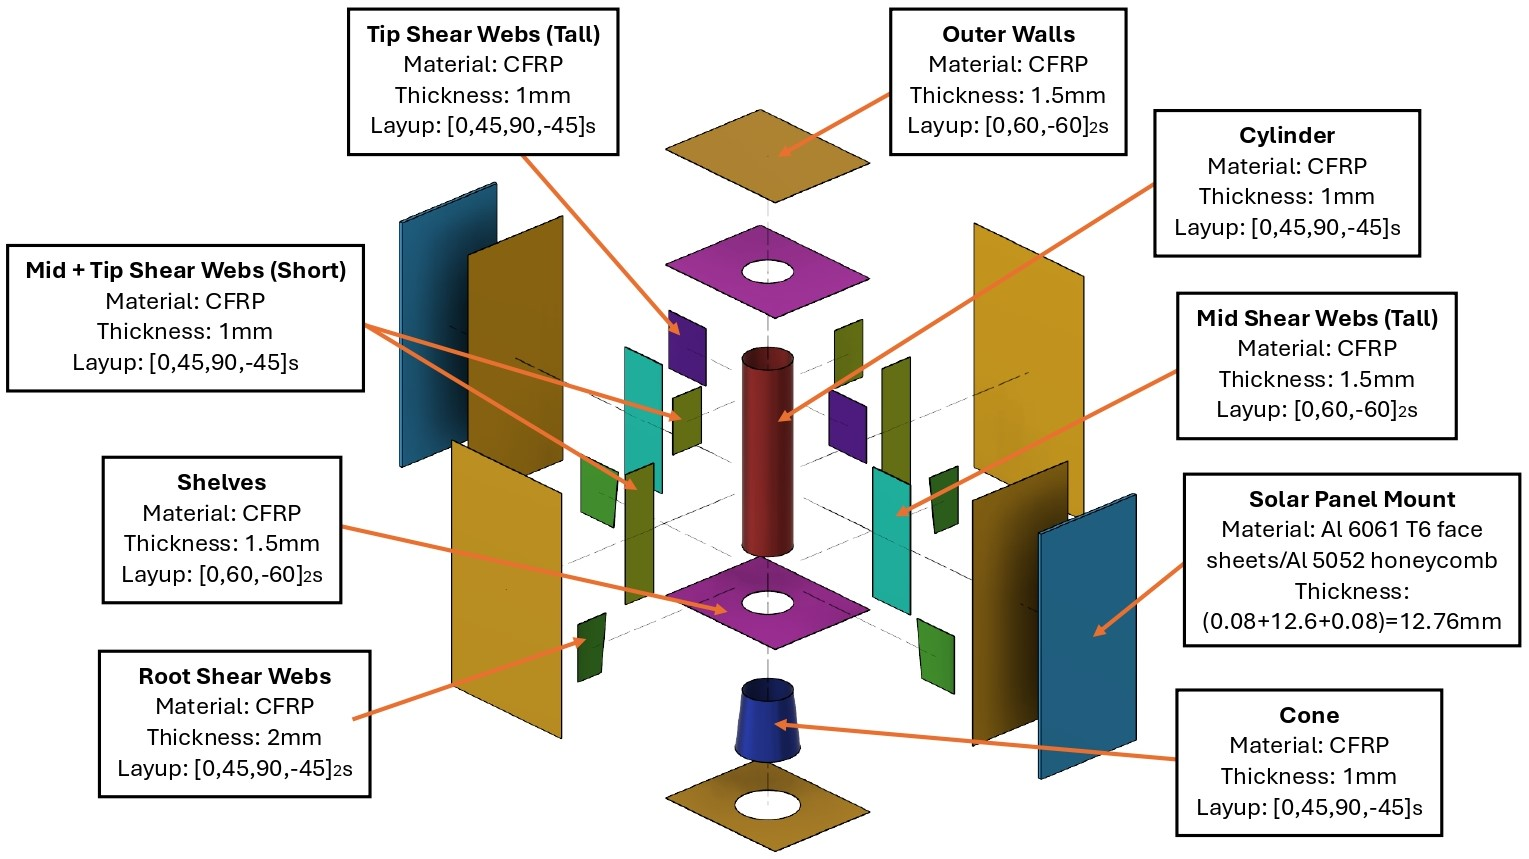
\includegraphics[width=0.8\textwidth]{figures/structural_assembly_exploded.jpg}
    \caption{Exploded view of structures}
    \label{structuresexploded}
\end{figure}

The following assumptions were made when sizing the structure:
\begin{itemize}
    \item The central column will carry the acceleration launch loads of the entire satellite mass, as well as thruster loads during operation.
    \item Shear webs will transfer the shear and axial loads from the cylinder to the rest of the structure, to reduce buckling of the central column. 
    \item Shelves act as ribs for the entire structure, providing torsional stiffness.
    \item The payload and magnetorquers are mounted to the shear webs.
    \item Outer walls carry the solar arrays and antenna mass.
    \item All other electronic equipment mounted to the shelves.
\end{itemize}
 
To efficiently transfer loads from the launcher, the diameter of the root of the cone has been matched to that of the separation ring. Then to optimise mass and volume, the cone tapers down to the diameter of the cylinder, which extends to the outer wall. The central cylinder was sized for tensile strength, natural frequency and buckling strength with an equivalent axial load of the primary load case, as suggested in SMAD \cite{wertz_space_1999}. Moreover, the cone was assumed to be an equivalent cylinder due to the slant angle being below 10° \cite{NASA_SP8019_1968}, but was later designed according to Roark's formulas \cite{young2002roark}. The shear webs were incorporated and sized using the parallel axis theorem, with further checks for panel stability. The shear webs taper down in thickness further away from the root to reduce mass. The force applied to the shelves and outer walls were calculated according to mass mounted and g-loading, then checked for panel stability based on their respective buckling coefficients \cite{Wijker2008}. All flat plates have also been checked for their natural frequency based on their respective boundary conditions \cite{blevins1979frequencyformulas}. Finally, the honeycomb panels were designed to avoid resonance \cite{Leissa1969VibrationOfPlates}, optimising for mass whilst checking for strength and buckling failures of the face and core \cite{Wijker2008}. During sizing, ELamX$^{2}$ was used to calculate engineering constants of the different layups, with the closest manufacturable thickness to the calculated value being chosen.



\subsubsection{Finite Element Analysis}

Finite Element Analysis was conducted in ABAQUS, using S4R 2D shell elements to build the structure. Components were modelled then merged into a single part to allow the nodes on the boundary of joining parts to be coincident with each other, thus improving the result accuracy. Simple cases were compared to analytical solutions, validating the FEA modelling methodology as seen in \autoref{tab:validation_final}. This was followed by a mesh sensitivity analysis of the entire model. This was achieved by increasing mesh density to observe whether output variables converge, indicating a stable and accurate model as seen in \autoref{fig:displacement}.  A mesh size of $16\,\mathrm{mm}$ was utilised for the rest of the analysis, as any more mesh refinement would increase calculation time for negligible improvement in accuracy. Four different analyses were conducted: static analysis with quasi-static loads, implicit dynamic analysis with quasi-static and sine loads, modal analysis and a buckling analysis with combined quasi-static and dynamic loads. The final FEA results are stated in \autoref{tab:fea_results}, with Hashin failure criteria used to predicit composite failure more accurately.

\begin{figure}[H]
\centering

% First row - compact
\begin{subfigure}{0.48\textwidth}
    \centering
    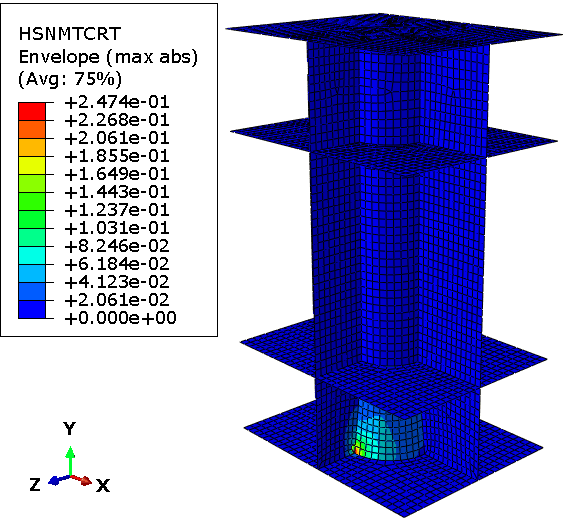
\includegraphics[width=0.7\linewidth]{figures/fea_matrix_tensile_hashin_failure.png}
    \caption{Matrix Tensile Hashin Failure Criteria for dynamic analysis}
\end{subfigure}
\hfill
\begin{subfigure}{0.48\textwidth}
    \centering
    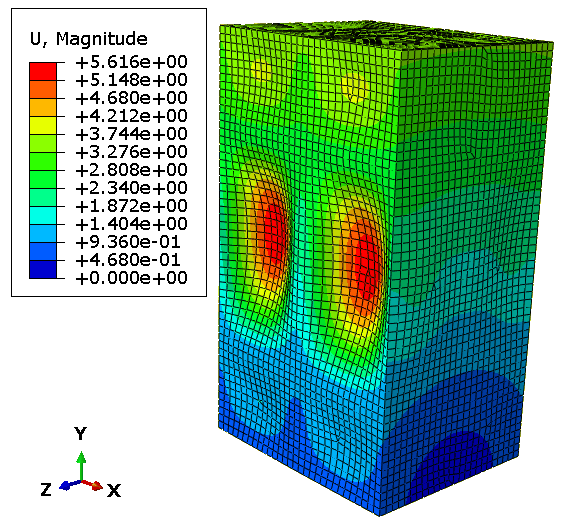
\includegraphics[width=0.7\linewidth]{figures/fea_maximum_deflection.png}
    \caption{Maximum Deflection for dynamic analysis}
\end{subfigure}

% Small vertical space
\vspace{0.2cm}

% Second row - compact
\begin{subfigure}{0.48\textwidth}
    \centering
    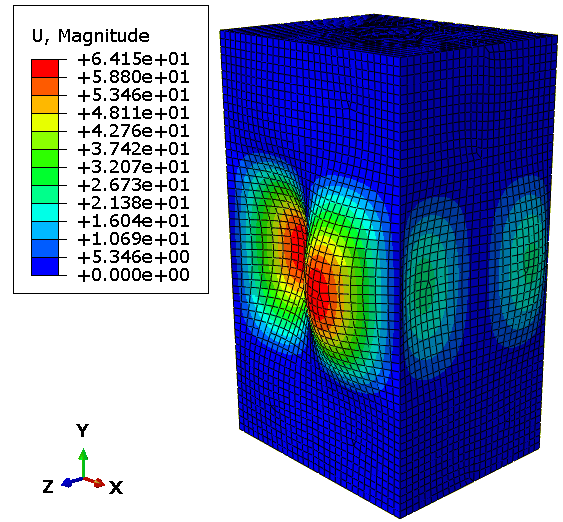
\includegraphics[width=0.7\linewidth]{figures/fea_first_vibration_mode.png}
    \caption{1st Vibration Mode for modal analysis}
\end{subfigure}
\hfill
\begin{subfigure}{0.48\textwidth}
    \centering
    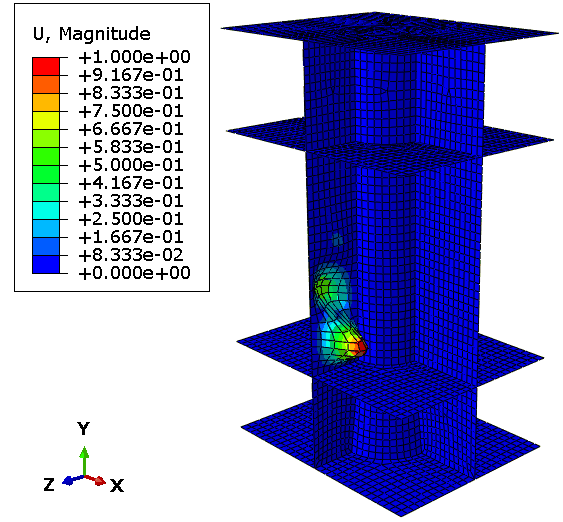
\includegraphics[width=0.7\linewidth]{figures/fea_first_buckling_mode.png}
    \caption{1st Buckling Mode for buckling analysis}
\end{subfigure}

\caption{Contour Plots of Key Analyses}
\end{figure}

\begin{table}[h!]
\centering
\caption{FEA Results}
\label{tab:fea_results}
\begin{tabular}{cccccc}
\toprule
Max. Stress (MPa) & Max. Deflection (mm) & Buckling RF & Stress RF & Hashin Failure RF & Vibration RF \\
\midrule
637 & 5.62 & 1.19 & 4.02 & 4.05 & 2.69 \\
\bottomrule
\end{tabular}
\end{table}


\begin{table}[H]
\centering
\caption{Hand Calculation vs FEA Validation}
\label{tab:validation_final}
\begin{tabular}{@{}>{\bfseries}l l c c c@{}}
\toprule
\textbf{Case} & \textbf{Variable} & \textbf{Hand Calc} & \textbf{FEA} & \textbf{\% Diff} \\
\midrule
Cylinder & Stress (MPa) & 273 & 267 & -2.2 \\
         & Deflection (mm) & 9.9 & 11.0 & 11.4 \\
         & Natural Frequency (Hz) & 35.4 & 33.0 & -6.5 \\
\midrule

Cylinder + Shear Webs & Stress (MPa) & 73.5 & 82.0 & 11.6 \\
                      & Deflection (mm) & 2.5 & 2.8 & 8.6 \\
\midrule

Cone & Stress (MPa) & 171 & 165 & -3.4 \\
\midrule

Sandwich Panel & Natural Frequency (Hz) & 52.9 & 44.7 & -15.5 \\
\bottomrule
\end{tabular}
\end{table}



\begin{figure}[H]
\centering
\begin{minipage}{0.6\textwidth}
\centering
\begin{tikzpicture}
\begin{axis}[
    width=\linewidth,
    height=5cm,
    xlabel={Element No ($\times 10^3$)},
    ylabel={Displacement (mm)},
    grid=major,
    xmin=0,
    xmax=35000,
    ymin=3.08,
    ymax=3.18,
    % Scientific notation options
    scaled x ticks=base 10:-3, % Divide by 10^3
    xtick scale label code/.code={}, % Remove the automatic "×10^3" label
    xtick={0, 5000, 10000, 15000, 20000, 25000, 30000, 35000},
    xticklabel style={/pgf/number format/.cd, use comma, precision=1},
    ytick={3.08,3.10,3.12,3.14,3.16,3.18},
]

\addplot[
    color=blue,
    mark=*,
    mark size=2pt,
    line width=1pt
] table[x=Element No,y=Displacement,col sep=comma] {data/fea_mesh_convergence.csv};

\end{axis}
\end{tikzpicture}
\caption{Displacement Convergence Plot}
\label{fig:displacement}
\end{minipage}
\hfill
% Right: 2x2 grid with image files and subcaptions
\begin{minipage}{0.32\textwidth}
\centering

% First row of 2x2 grid
\begin{subfigure}{0.48\textwidth}
\centering
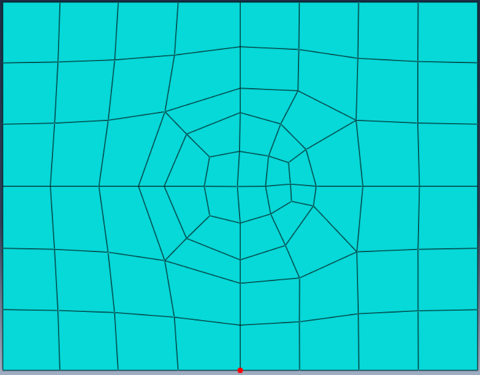
\includegraphics[width=\linewidth, height=0.75\linewidth]{figures/fea_mesh_940_elements.png} % Replace with your image file
\caption{940 Elements}
\label{fig:sub1}
\end{subfigure}
\hfill
\begin{subfigure}{0.48\textwidth}
\centering
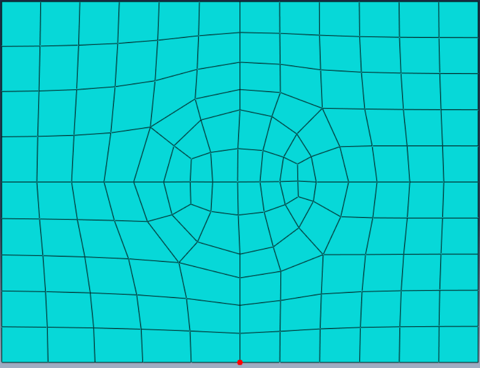
\includegraphics[width=\linewidth, height=0.75\linewidth]{figures/fea_mesh_2129_elements.png} % Replace with your image file
\caption{2129 elements}
\label{fig:sub2}
\end{subfigure}

\vspace{0.3cm}

% Second row of 2x2 grid
\begin{subfigure}{0.48\textwidth}
\centering
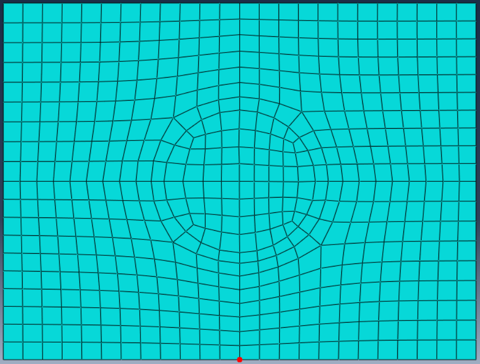
\includegraphics[width=\linewidth, height=0.75\linewidth]{figures/fea_mesh_8370_elements.png} % Replace with your image file
\caption{8370 elements}
\label{fig:sub3}
\end{subfigure}
\hfill
\begin{subfigure}{0.48\textwidth}
\centering
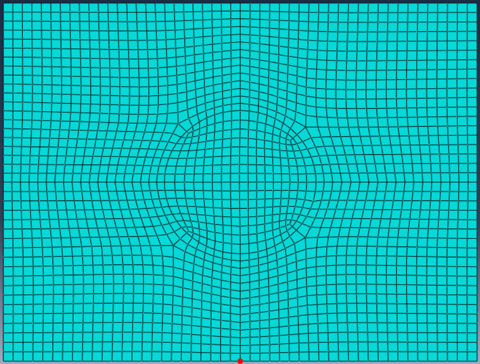
\includegraphics[width=\linewidth, height=0.75\linewidth]{figures/fea_mesh_32534_elements.png} % Replace with your image file
\caption{32534 elements}
\label{fig:sub4}
\end{subfigure}

\caption{Mesh density}
\label{fig:analysis_grid}
\end{minipage}
\end{figure}





\subsection{Attitude and Orbit Control System}
The AOCS equipment consists of entirely COTS components, chosen to minimise the number of suppliers, and maximise reliability and heritage. This allows for easier coordination of lead times, simplified system integration and more consistent manufacturer support. CubeSpace was chosen for computing, sensing, and actuation, while SkyFox Labs was chosen for GNSS modules. 
\subsubsection{Actuator Selection and Sizing}
Actuator sizing was decided by taking into account worst-case disturbance torques, with verification by way of a Monte Carlo study for nominal operations.

Typical disturbance torques at the selected orbit and altitude were modelled in a triangular distribution. Aerodynamic drag, gravity gradient, residual magnetic dipole, and solar radiation pressure disturbances were considered. Values for these disturbances were derived from  variations in atmospheric quantities, such as density for aerodynamic drag and solar flux for SRP \cite{EMMERT2015773,kopp-2016}. The magnitude of these disturbances can be seen clearly in \autoref{fig:distorque}, and were then compared with the maximum available MTQ output along the disturbance direction as shown in \autoref{fig:mtqdist}:

\begin{figure}[H]
    \centering
    \begin{minipage}{0.4\textwidth}
        \centering
        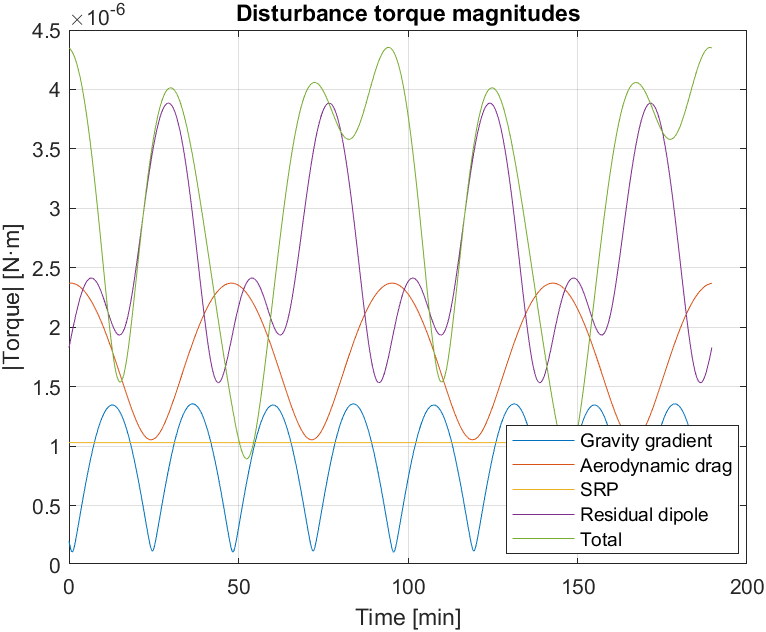
\includegraphics[width=\linewidth]{figures/aocs_disturbance_torques.png}
        \caption{All modeled disturbances}
        \label{fig:distorque}
    \end{minipage}\hfill
    \begin{minipage}{0.4\textwidth}
        \centering
        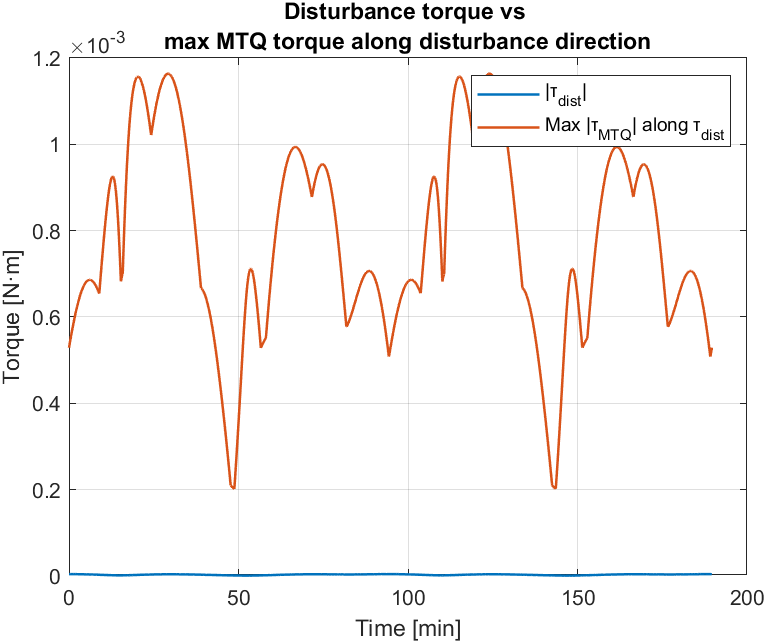
\includegraphics[width=\linewidth]{figures/magnetorquer_authority_vs_disturbances.png}
        \caption{MTQ compared with disturbances}
        \label{fig:mtqdist}
    \end{minipage}
\end{figure}

However, it should be noted that a direct comparison of torques is not enough to validate the design. The continuous closed-loop performance must also be evaluated, to see how it interacts with torques that build up over time. This was done using a Monte Carlo simulation study that measured microgravity at a point in the payload furthest from the COM, as shown in \autoref{fig:montecarlomtq}:
\begin{figure}[H]
    \centering
    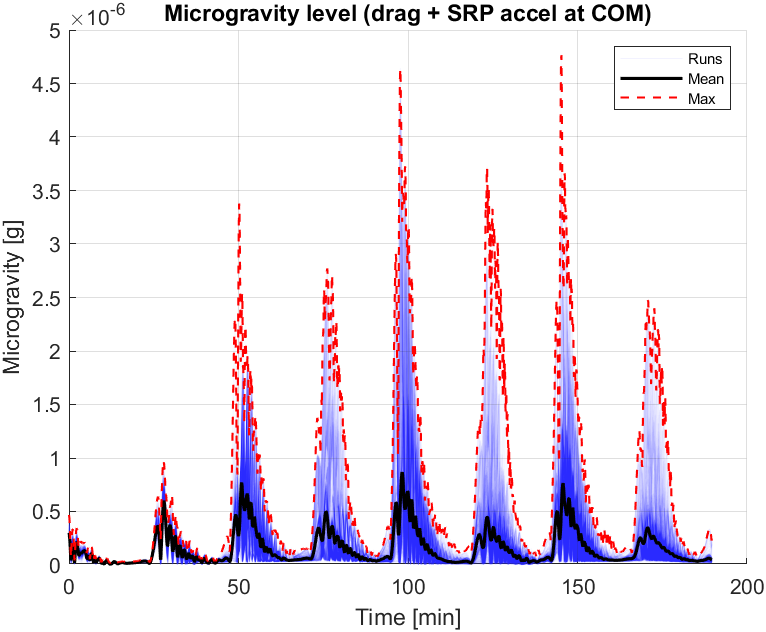
\includegraphics[width=0.4\linewidth]{figures/nominal_control_monte_carlo_microgravity.png}
    \caption{Monte Carlo simulation results in nominal operations}
    \label{fig:montecarlomtq}
\end{figure}

\subsubsection{Sensor Selection}
Most COTS sensors on the market are well within the pointing requirements as set out by Space Forge, as well as the derived requirements detailed by SerenSpace. However, these were quantified and compared for thoroughness.

\textbf{Sun Sensors:} The chosen sun sensor's maximum slew rate of $70^\circ\,\mathrm{s}^{-1}$ as specified in the Cubesense Sun datasheet \cite{cubespace-2023} is more than accommodating of the maximum expected slew rate of $0.7^\circ\,\mathrm{s}^{-1}$ in nominal operations as measured from the Monte Carlo study, leaving plenty of margin for attitude sensing. Using two of them also provides redundancy and better coverage.

\textbf{Star Trackers:} Unlike the sun sensors, the star trackers will be used primarily to continuously calibrate the IMU. Hence, it need not be always functional. The chosen star tracker has a maximum operable slew rate of $0.3^\circ\,\mathrm{s}^{-1}$, which while smaller than the maximum expected slew rate during nominal operations, is still larger than the average slew rate. This allows us to repeatedly calibrate the IMU at least once per minute. The accuracy of the star tracker leaves a large amount of margin for the calibration of the IMU and magnetometer with absolute attitude updates.

\textbf{Magnetometer:} The closed-loop control sensor needs for the MTQ-only control regime using a PD controller can be described using its signal to noise ratio (SNR) of $\approx50.4\,\mathrm{dB}$ \cite{rojas-2008}. To have stable pointing, this needs to be above $15\,\mathrm{dB}$, which the chosen magnetometer exhibits with margin.

\textbf{GNSS:} The GNSS receiver and antennas were selected to comply with SFG-REQ-190, and together have a measurement accuracy of $<10\,\mathrm{m}$ and $<1\,\mathrm{m\,s}^{-1}$ during the entirety of the mission.

\subsubsection{Control Architecture}
A heritage PD controller was used for simulations, although it would be feasible to implement an LQR with a Kalman filter as a state estimator due to the simple dynamics of the platform. 

\begin{figure}[H]
    \centering
    \resizebox{0.9\linewidth}{!}{%
        \tikzset{
  block/.style={draw, thick, minimum width=30mm, minimum height=11mm, align=center},
  sum/.style  ={circle, draw, thick, inner sep=0pt, minimum size=6mm},
  line/.style ={-Latex, thick},
  small/.style={font=\footnotesize}
}

\begin{tikzpicture}[x=1mm,y=1mm]

\node[block] (mode)  at (0,0)                 {Mode Manager};
\node[block] (guid)  at (45,0)                {Guidance\\\small $q_{ref},\,\omega_{ref}$};
\node[sum]   (sum1)  at (80,0)                {}; 
\node[block] (ctrl)  at (125,0)               {Controller\\\small PD / LQR};
\node[block] (alloc) at (165,0)               {Actuator Allocation};

\node[block] (plant) at (215,0)               {S/C Dynamics\\\small $J\dot\omega = \tau_{\text{cmd}} + \tau_{\text{dist}} - \omega \times J\omega$};
\node[block] (dist)  at (215,22)              {Disturbances\\\small $T_{gg}, T_{drag}, T_{SRP}, T_{mag}$};

\node[block] (sens)  at (215,-26)             {Sensors \& Noise\\\small ST / SS / IMU / MTM / GNSS};
\node[block] (est)   at (165,-26)             {Estimator (EKF/UKF)\\\small $\hat q,\,\hat\omega,\,\hat b_g$};

\node[block] (sel)   at (165,-50)             {Sensor Selection};
\node[block] (mom)   at (125,-15)             {Momentum\\Management};

\draw[line] (mode.east)  -- (guid.west);
\draw[line] (guid.east)  -- (sum1.west);
\draw[line] (sum1.east)  -- node[above,small] {$e_q,\,e_\omega$} (ctrl.west);
\draw[line] (ctrl.east)  -- (alloc.west);
\draw[line] (alloc.east) -- node[above,small] {$\tau_{\text{cmd}}$} (plant.west);

\draw[line] (dist.south) -- (plant.north);

\draw[line] (plant.south) -- (sens.north);
\draw[line] (sens.west)   -- (est.east);

\draw[line] (est.south) -- (sel.north);
\draw[line] (ctrl.south) -- (mom.north);

\coordinate (fb_left) at (est.west -| sum1.south);
\coordinate (mom_right) at (mom.east -| alloc.south);
\coordinate (mode_up) at ($(mode.north)+(0,10)$);
\coordinate (mode_down) at (mode.south |- sel.west);

\draw[line] (est.west) -- (fb_left) -- (sum1.south);
\draw[line] (mom.east) -- (mom_right) -- (alloc.south);
\draw[line] (mode.north) -- (mode_up) -- (mode_up -| ctrl.north) -- (ctrl.north);
\draw[line] (mode.north) -- (mode_up) -- (mode_up -| alloc.north) -- (alloc.north);
\draw[line] (mode.south) -- (mode_down) -- (sel.west);

\node[small] at ($(sum1.south)+(3,-3)$) {$-$};
\node[small] at ($(sum1.west)+(-3,3)$) {$+$};

\end{tikzpicture}%
    }
    \caption{Top-level control block diagram of SCIPIO–1}
    \label{fig:controlblock}
\end{figure}

\subsection{Propulsion}
\subsubsection{Thruster Selection}
To meet the platform's propulsion needs, an in-depth review of several thrusters was conducted. General properties including thrust and propellant were decided first—it would not have been constructive to compare a $1\,\mathrm{N}$ monopropellant thruster with a $220\,\mathrm{N}$ bipropellant. This was followed by an MCDA down-selection, which narrowed the choice down to a Rafael $5\,\mathrm{N}$ thruster.

A thrust range of approximately $5-10\,\mathrm{N}$ was selected. This was a trade-off between being high enough to provide a precise deorbit burn, whilst not being so large that torque misalignment would be beyond AOCS’ detumble capability. A stronger but shorter burn offers a reduced landing ellipse area; deorbit into an uninhabited area (SPOUA) can therefore be guaranteed.

A monopropellant architecture was selected for the mission; the improved ISP of bipropellant and the simplicity of cold gas could not be justified over their higher complexity and poor performance, respectively. There are 3 primary categories of monopropellant to choose from: Peroxide (HTP), Hydrazine (\ce{N2H4}), and green propellants. All three show heritage and offer a similar ISP($\approx200\,\mathrm{s}$), with Peroxide fairing slightly worse. All three carry disadvantages, albeit different ones with different implications for the mission. Hydrazine is highly carcinogenic and toxic; however, 80 years of heritage has resulted in thorough standards and precautions today. HTP is unstable over long periods and decomposes into water and oxygen. This results in the dangerous increase of tank pressure over time. Missions over 60 days require further qualifying by Falcon 9 \cite{noauthor_falcon9rideshare_2024}. HTP was  ruled out to avoid this complication. LMP-103s is a greener, safer alternative to Hydrazine. Despite offering a $6\%$ ISP increase \cite{ECAPS_LMP103S_2023}, it cannot be cold started and has a greater power draw, heating the catalyst bed in excess of $350^{\circ}\,\mathrm{C}$. Under LMP-103s, the heater acts as a single point of failure for the propulsion system. In spite of its toxicity, Hydrazine was chosen for its ISP, stability over a long mission, and a lower power requirement.

An MCDA down-selection was conducted for four TRL-9 Hydrazine compatible thrusters in the $5-10\,\mathrm{N}$ range. They were evaluated with respect to five properties: mass, volume, power draw, ISP, and minimum impulse bit. These properties' weightings were identified through a pairwise comparison. Thrusters were scored by their relative distance from the mean value in each category. The MCDA shown in \autoref{tab:thrusterdownselection} indicates the ultimate selection of the Rafael $5\,\mathrm{N}$ thruster.

\begin{table}[H]
\centering
\caption{MCDA Downselection resulting in the Rafael $5\,\mathrm{N}$ thruster}
\label{tab:thrusterdownselection}
\begin{tabular}{l *{9}{c}}
\toprule
\multirow{2}{*}{Criteria} & 
\multirow{2}{*}{Weightings} & 
\multicolumn{2}{c}{Ariane $5\,\mathrm{N}$} & 
\multicolumn{2}{c}{\cellcolor{yellow!25}Rafael $5\,\mathrm{N}$} & 
\multicolumn{2}{c}{L3Harris MR-111G} & 
\multicolumn{2}{c}{Moog MONARC-5} \\
\cmidrule(lr){3-4} \cmidrule(lr){5-6} \cmidrule(lr){7-8} \cmidrule(lr){9-10}
 & & score & weighted & score & \cellcolor{yellow!25}weighted & score & weighted & score & weighted \\
 & & & score & & \cellcolor{yellow!25}score & & score & & score \\
\midrule
Mass & 0.46 & 5 & 2.3 & 8 & \cellcolor{yellow!25}3.6 & 6 & 2.7 & 2 & 0.9 \\
Volume & 0.21 & 5 & 1.0 & 5 & \cellcolor{yellow!25}1.0 & 5 & 1.0 & 5 & 1.0 \\
ISP & 0.11 & 2 & 0.2 & 4 & \cellcolor{yellow!25}0.5 & 7 & 0.8 & 7 & 0.8 \\
Power Draw & 0.17 & 5 & 0.9 & 4 & \cellcolor{yellow!25}0.7 & 7 & 1.2 & 5 & 0.9 \\
Min. Impulse bit & 0.05 & 6 & 0.3 & 8 & \cellcolor{yellow!25}0.4 & 2 & 0.1 & 5 & 0.3 \\
\midrule
Total & 1 & & 4.7 & & \cellcolor{yellow!25}6.2 & & 5.9 & & 3.9 \\
\bottomrule
\end{tabular}
\end{table}

\subsubsection{Feed System}
Beyond the stringent safety requirements mandated by Falcon 9, the feed system was driven by compact volume and low mass, enabling it to fit within the (158 mm internal diameter) cylindrical primary load structure. The propulsion system was thus designed to be fully contained; the feed lines remain within this structure. It would be assembled separately, then slid into the platform for AIT. The propellant and nitrogen fill lines are accessible from the bottom, with ample space either side of the thruster. This design philosophy guarantees piping will not breach the cylinder wall, thereby avoiding further stress concentrations in the primary load structure.

An entirely blowdown system was investigated, which would reduce mass and complexity. However, initial calculations demonstrated considerable pressure ‘droop’, such that the thruster would operate at approximately $1\,\mathrm{N}$ at the end of a steady state burn $(t = T_b)$. To avoid this unfavourable characteristic, an inert pressuring tank with a downstream regulator was deemed necessary.

Instead of Gaseous Helium (GHe), Gaseous Nitrogen (GN$_2$) was chosen for pressurisation. This decision is again driven by the volume constraint. To avoid leakage, GHe COPVs often are larger in volume and operate at a lower MEOP. Selecting GN$_2$ resulted in a leak-resistant higher pressure feed system, but with a much smaller vessel. GN$_2$ is heavier per mole than GHe; however, the mass of pressurant required is only in the order of grams. This, in turn, results in a net mass savings by choosing smaller tanks. One disadvantage is that GN$_2$ absorbs into fuels, which can be mitigated with a bladder tank. Employing GN$_2$ is not a novel solution to spacecraft, with the Compton Gamma Ray Observatory spacecraft \cite{NASA1991_GRO_MOR} also employing it.

LMO Space’s PBT-3 Hydrazine Bladder tank was selected; bladder tanks are a heritage method of managing propellant pressure. With a moderate weight of $1.75\,\mathrm{kg}$, this tank can hold $3.1\,\mathrm{L}$ of propellant, addressing the mission’s delta-V requirement, see \autoref{sub:deltav}. Additionally, the tank’s MEOP is $24\,\mathrm{bar}$, resulting in a high chamber pressure and subsequent ISP. The COPV is a type 3 composite vessel. Typically, composite tanks carry further restrictions regarding flight worthiness; however, being from an American company (Aerojet Rocketdyne) it would be US DOT (Department of Transport) approved, though it could still be at risk of ITAR restrictions.

The rest of the feed system components were selected for compliance with a Falcon 9 rideshare. The shape memory alloy valves on the high-pressure line are rated to $330\,\mathrm{bar}$ far exceeding the systems MEOP. Similarly, the latching solenoid valves have a proof pressure of $36\,\mathrm{bar}$; with MEOP at 24, it demonstrates the required $1.5\times$ safety factor. Additionally, contingency relief is exhibited in the P\&ID, see \autoref{fig:Feedsystem}, with burst disks on both the high- and low-pressure lines. Addressing single-fault tolerance of propellant release (PRP-REQ-038), the latching solenoid valves are in series and would actuate by separate electrical commands.

\begin{figure}[H]
    \centering
    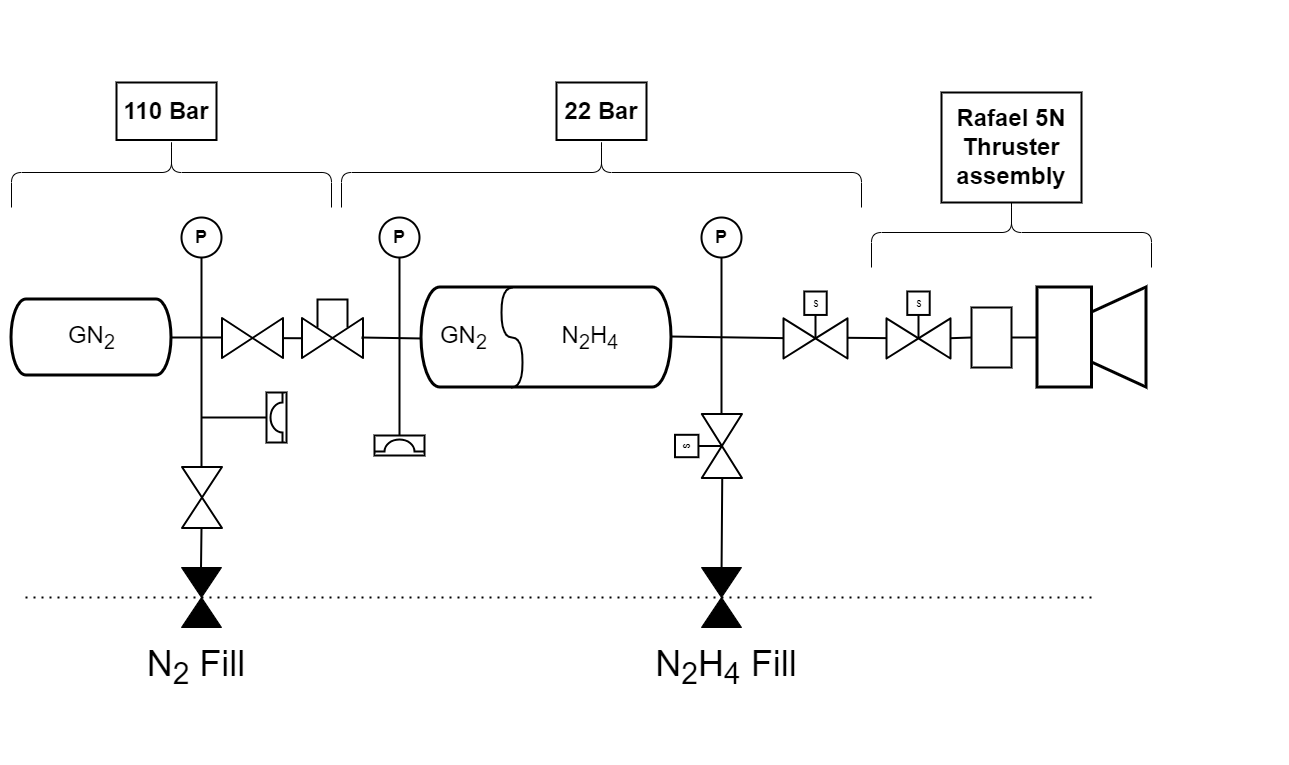
\includegraphics[width=0.6\linewidth]{figures/propulsion_feed_system_pid.png}
    \caption{P\&ID of the Propulsion System}
    \label{fig:Feedsystem}
\end{figure}

\subsubsection{Thruster Analysis}
Calculations were performed on the thruster with two distinct goals. The first was to determine the tank pressurisation requirement. The second was to estimate the key thruster parameters ($P_c$, ISP, and Thrust) to a higher fidelity than the data sheet. These values were fed back into DRAMA and STK to ensure there was sufficient propellant mass for deorbit and collision avoidance, thus further refining SCIPIO-1’s delta-V budget.



The tank pressurisation requirement was found using the Ideal Gas Equation. Based on thermal estimates, the tank is assumed to be at $293\,\mathrm{K}$. The COPV must maintain the PBT-3 tank at $24\,\mathrm{bar}$ until it has completely expelled the Hydrazine, ensuring that the thruster operates at maximum ISP/thrust at the end of the deorbit burn. The COPV's pressure drops as GN$_2$ is expelled through the regulator; the pressure must remain constant on the other side of the regulator. A MATLAB simulation was performed to determine the chamber pressure (and the resulting ISP/thrust) at the end of a deorbit burn, as a function of the COPV's initial pressurization. \autoref{fig:Thrusteranalysis} indicates that, due to the regulator, there is no need to pressurize the COPV beyond $110\,\mathrm{bar}$. The ideal gas equation also indicates only $120\,\mathrm{g}$ of GN$_2$ is needed for this.

\begin{figure}[H]
    \centering
    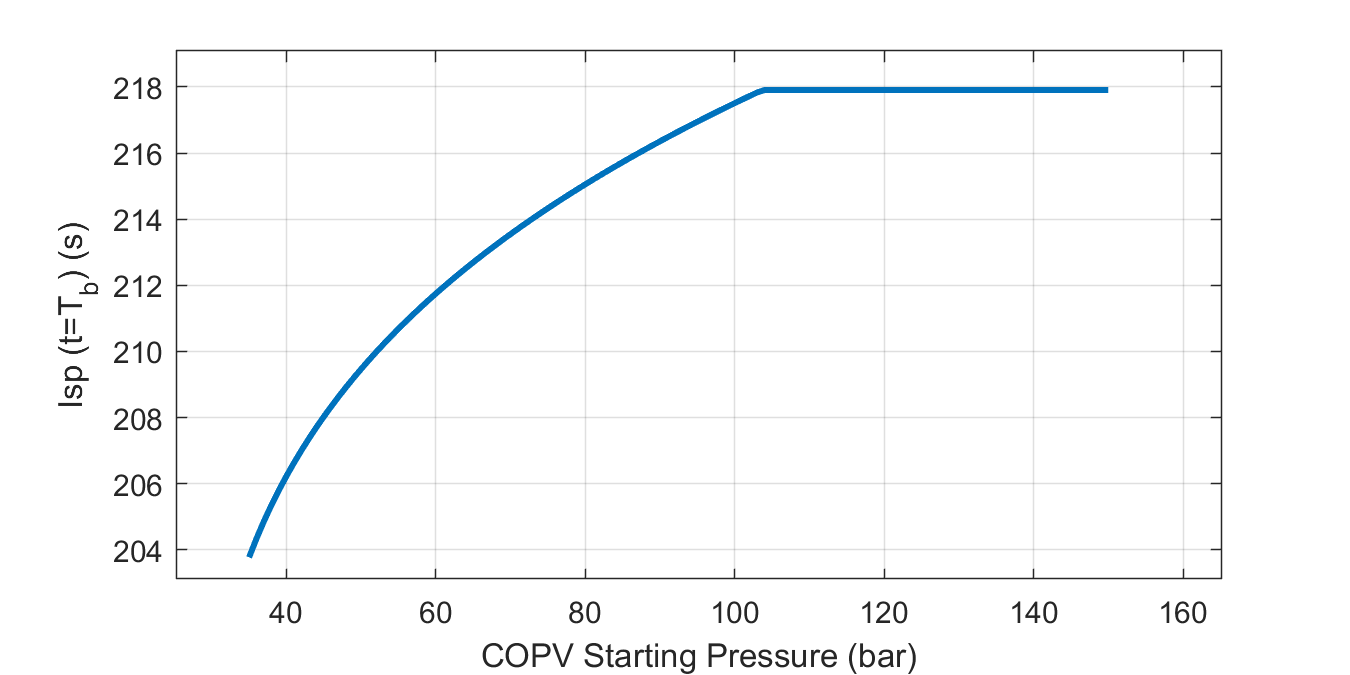
\includegraphics[width=0.6\linewidth]{figures/specific_impulse_vs_copv_pressure.png}
    \caption{A plot of ISP at $t=T_b$, as a Function of COPV Pressurisation}
    \label{fig:Thrusteranalysis}
\end{figure}

Thruster inlet pressure was then solved with conservative estimates of pressure drop through $0.35\,\mathrm{m}$ of \sfrac{1}{4} inch pipe. \autoref{eq:darcy_weisbach} (the Darcy-Weisbach equation for turbulent flow) was used to solve this, where the friction coefficient $\lambda = 0.058$. A $20\%$ pressure drop over the injector and catalyst was assumed to determine chamber pressure.

\begin{equation}
\Delta{P_{loss}} = \lambda \frac{l}{D} \frac{\rho v^2}{2}
\label{eq:darcy_weisbach}
\end{equation}

Under Ideal rocket equations, ISP and thrust can be assumed proportional to the thruster exit velocity ($V_e$). Using \autoref{eq:exit_velocity} and a heat capacity ratio ($\gamma$) of $1.25$ for Hydrazine, it can be determined that Ve, ISP and thrust are proportional to $P_c^{1/4}$. With this relation an interpolation of datasheet values for thrust and ISP could be performed, resulting in final values of $4.7\,\mathrm{N}$ and $217\,\mathrm{m\,s}^{-1}$, respectively.

\begin{equation}
\upsilon_e = \sqrt{\frac{2\gamma}{\gamma-1}\frac{R_A}{M_W}T_C \left[ 1 - \left(\frac{p_e}{p_C}\right)^{\frac{\gamma-1}{\gamma}} \right]}
\label{eq:exit_velocity}
\end{equation}

\subsection{Communications and OBDH}
\label{sub:comms_obdh_TR}
\subsubsection{Ground station}
Initially, two UHF ground stations were selected to meet the 2 hour and 4 hour cadence requirements (SFG-REQ-310) (SFG-REQ-290), namely Bardufoss, Norway and Fairbanks, USA. However, following Space Forge's suggestion to use full ground station networks, SCIPIO-1 utilises the full Terran network as shown in \autoref{fig:Terran} in green. The Terran network was modelled in STK using link margin in \autoref{tab:fedr_link_budget}.  The critical access time is confirmed in \autoref{fig:urmom} and the data requirements in \autoref{tab:data_budget_STK} reflect the total downlinkable data for critical and bulk telemetry. Additionally, the Terran network also offers services from partner ground stations, giving access to an additional twelve S-band ground stations as shown in figure \ref{fig:Terran} in orange allowing for flexible choice of operations in case ground stations become unavailable.
\begin{figure}[H]
    \centering
    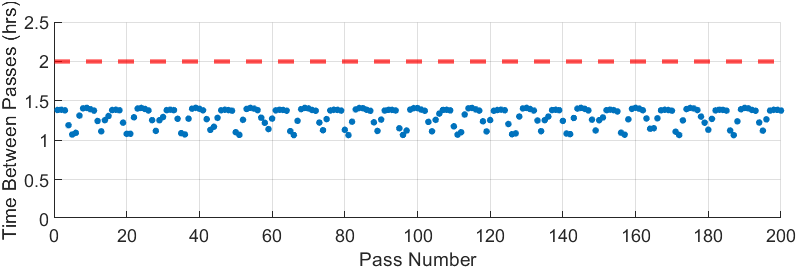
\includegraphics[width=0.7\linewidth]{figures/uhf_downlink_opportunities.png}
    \caption{UHF Downlink Opportunities}
    \label{fig:urmom}
\end{figure}

\subsubsection{Transmission Frequency Selection}
As outlined in the mission report, critical telemetry is transmitted through a UHF frequency of $400\,\mathrm{MHz}$  because of the frequency's for enhanced fault tolerance, low attenuation properties and wide coverage. This would allow robust and consistent communication with the ground station, increasing confidence in meeting SFG-REQ-260 and SFG-REQ-310. The S-Band frequency is chosen for its high data rate capabilities and relatively low attenuation properties. The S-Band frequencies for transmitting and receiving are separated into $2.250\,\mathrm{GHz}$ and $2.075\,\mathrm{GHz}$ respectively. This minimise interference and align with the ground station operational frequencies.
\subsubsection{Components Selection}
The communication components were selected from the State-of-the-Art of Small Spacecraft Technology handbook \cite{nasaCommunicationsNASA}. As shown in figure \ref{fig:component_configuration} the communication subsystem uses two UHF antennas on the $\pm$Z faces. This is to establish communications during detumbling and optimize communication for the high latitude ground stations. The S-band antennas are placed on the $\pm$Y faces of the satellite to maximise coverage with the lower latitude S-band ground stations and accommodate the interial fixing requirements. Following the frequency down selection process, the Space manic Murgas Radio was selected for UHF communication as it meets the critical data uplink requirements. Afterwards, Space manic SAM antenna because it offers the same polarisation to the ground stations and is of the same origin as the Murgas UHF radio, indicating easier integration between components. The Slink-Phy S-band transceiver was chosen for its high data rate and full duplex capabilities to meet the full duplex requirement; the Anywaves TT\&C S-band antenna was chosen for its high gain and hemispherical coverage, increasing access time.
\subsubsection{Modulation Selection}
Based on component selection and ground station capabilities, the UHF communications system uses GMSK modulation for both uplink and downlink. For critical communication, GMSK modulation is chosen because of its high mainlobe to sidelobe suppression \cite{wertz_space_1999}, resulting in high efficiency and low interference. The S-band communication system QPSK modulation for downlinks and BPSK for uplinks. QPSK modulation is favourable for downlink because of its high spectral efficiency with relatively low bit error rate. In terms of using BPSK, it is more robust to noise and interference because of its two-phase modulation. 
\subsubsection{Link Analysis}
The link margin is key to verifying that communication can be established between the satellite and the ground station. \autoref{tab:linkbudget_clean} shows the link margins during uplink and downlink of both UHF and S-Band frequencies. \autoref{tab:fedr_link_budget} shows the detailed link budget and \autoref{tab:link_budget_assumptions} shows the losses and gains assumptions during all stages of communication.
\begin{table}[h]
    \centering
    \caption{Link Budget Properties}
    \label{tab:link_budget_assumptions}
    % Corrected: Removed \mathbf{} from around \textwidth
    \begin{tabularx}{\textwidth}{l X} 
        \toprule
        \textbf{Variable} & \textbf{Notes} \\
        \midrule
        % Group Header: Transmitter losses/gains
        \multicolumn{2}{l}{\textbf{Transmitter losses/gains}} \\ 
        \midrule
        EIRP & Using maximum power, transmitter power loss and antenna gain. Requires data sheet \\
        Bit Rate Loss & Detailed calculation shown in link budget. Compromise between high data transfer and link margin requirement depending on communication system \\
        \midrule
        % Group Header: Transmission losses
        \multicolumn{2}{l}{\textbf{Transmission losses}} \\
        \midrule
        Atmospheric Loss & Conservative estimation using SMAD theory assumptions \\
        Path Loss & Equation found in link budget. Uses conservative distances beyond orbit altitude to ensure maximum communication time \\
        \midrule
        % Group Header: Receiver losses/gains
        \multicolumn{2}{l}{\textbf{Receiver losses/gains}} \\
        \midrule
        Receiver system loss & SMAD theory assumption \\
        Required power & Dependent on modulation scheme. Using a design Bit Error Rate (BER) of $10^{-4}$ for accurate data transmission \\
        System Noise Density & Assuming $280\,\mathrm{K}$ operating temperature \\
        Receiver antenna gain & Dependent on communication architecture using data sheet information \\
        \midrule
        Link Margin & $6\,\mathrm{dB}$ ideal for near Earth communication \\
        \bottomrule
    \end{tabularx}
\end{table}
\subsubsection{Data Budget}


In order to estimate the data volume that could be downlinked in a day, an effective data rate was first calculated. This was achieved by applying the following losses to the transceiver data rates.

\begin{table}[H]
    \centering
    \caption{Data Transmission Losses}
    %\renewcommand{\arraystretch}{1} % Optional: increase row height
    \begin{tabularx}{0.8\linewidth}{l c X} 
        \toprule
        \textbf{Loss} & \textbf{\%} & \textbf{Notes} \\
        \midrule
        Packetisation Overheads & $21.8$ & Based on $1115$ Byte CCSDS Data Frames, filled with $256$ Bytes Data Packets, with Reed Solomon Bit Error Correction applied \\
        Loss due to Bit Error Rate & $0$ & Negligible after Reed Solomon Error Correction \\
        Loss during link & $10$ & Estimated loss to account for inefficient transmission of data frame\\
        Loss setting up link & $10$ & Estimated loss to account for time spent setting up the link\\ 
        \bottomrule
    \end{tabularx}
    \label{tab:Downlink_Losses}
\end{table}

Access analysis was then performed in STK to calculate total transmission time per day. To ensure that only viable links were included in access times, the following parameters from the link budget were applied to STK ``Sensor" objects:

\begin{table}[H]
    \centering
    \caption{STK Sensor Parameters}
    \renewcommand{\arraystretch}{1} % Optional: increase row height
    \begin{tabularx}{0.65\linewidth}{l c c c} 
        \toprule
          & \textbf{UHF Band} & \textbf{S-band} & \textbf{S-band (RDT Mode)} \\
        \midrule
        Range (km) & $3000$ & $3000$ & $2000$\\
        Field of View ($^\circ$) & $\pm180^\circ$ & $\pm60^\circ$ & $\pm30^\circ$ \\
        Satellite Pointing & Inertial Pointing & Inertial Pointing & Ground Tracking\\
        \bottomrule
    \end{tabularx}
    \label{tab:data_budget_STK}
\end{table}

 The generated access data was then processed to determine average access durations per pass and per day, as well as the time between passes. The data volume which could be transmitted within these periods was calculated by multiplying this duration by the effective data rate.

The data generated by the platform in a day was calculated for both nominal and safe operations; this is indicated in the appendix, see \autoref{tab:data_budget_nominal_orig}. Data rates for each component were calculated based on SMAD and datasheet values. Notably, some entries are $0\,\mathrm{MB/day}$ in safe mode, because they will not operate and therefore will not generate data. The data was then separated into bulk and critical, under guidance from SMAD. \autoref{fig:Nom_data_rates}, clearly indicate generous margins in the volume of critical and bulk data to downlink per day.

When historical telemetry requires downlinking, the Rapid Data Transfer Mode fulfils SCIPIO-1's daily downlink requirements. A data backlog scenario could be induced by the platform remaining in safe or collision mode for prolonged periods. In the RDT mode, 27 hours of bulk data can be downlinked within a single pass; \autoref{fig:rapid_transfer_downlink_margin} shows the additional capacity provided by this mode.

\begin{figure}[H]

\begin{subfigure}{0.5\textwidth}
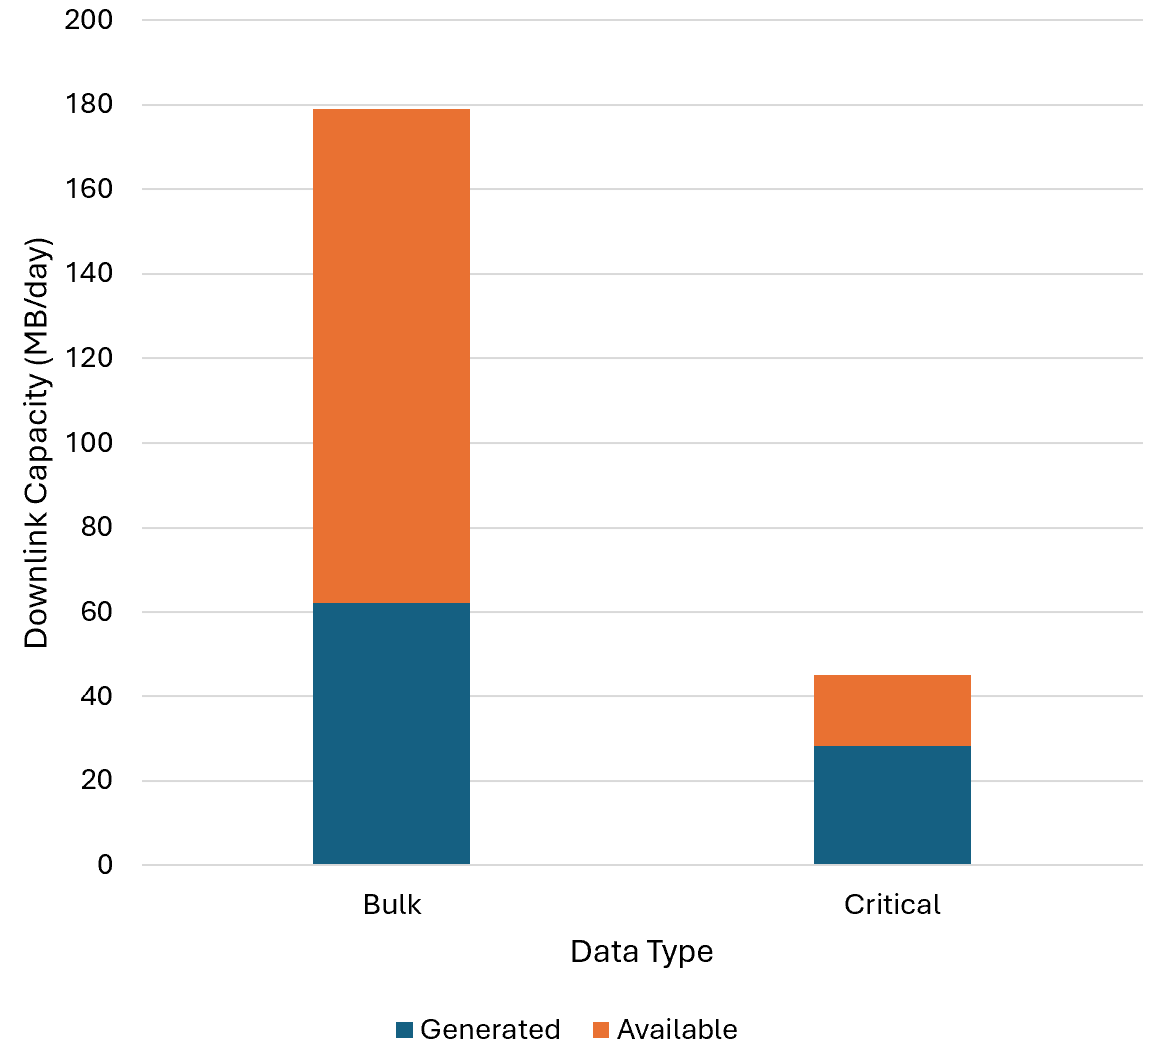
\includegraphics[width=0.9\linewidth, height=6cm]{figures/science_mode_downlink_margin.png} 
\caption{Science Mode}
\label{fig:Nom_data_rates}
\end{subfigure}
\begin{subfigure}{0.5\textwidth}
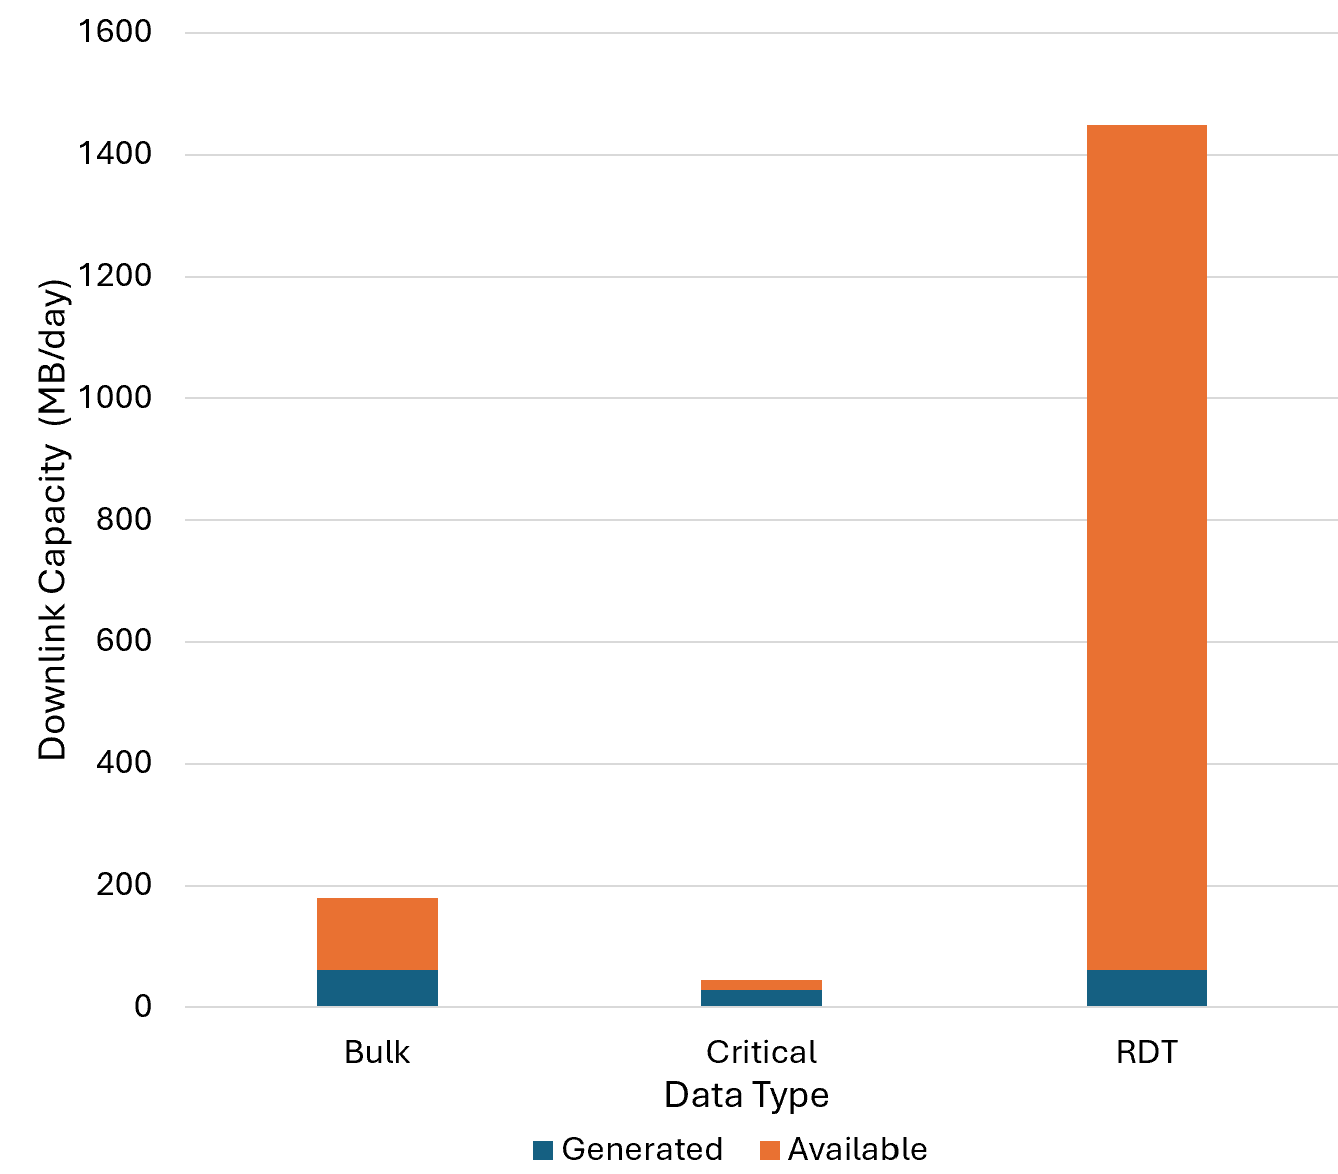
\includegraphics[width=0.9\linewidth, height=6cm]{figures/rapid_transfer_mode_downlink_margin.png}
\caption{Rapid Data Transfer Mode}
\label{fig:rapid_transfer_downlink_margin}
\end{subfigure}

\caption{Data Downlink Margins Under Different Modes}
\label{fig:image2}
\end{figure}

\subsection{Power}
 The primary design driver for the subsystem is SFG-REQ-240, requiring all power to be generated from solar energy. Alongside, were the derived requirements (PLP-REQ-073, PLP-REQ-074, PLP-REQ-075) ensuring compliant power delivery to the mission’s primary payload. The power system was designed with full redundancy, with limiting cases and conservative margins applied during all budgeting considerations. As such, the EPS confidently ensures compliance with all mission requirements, with the overall proposed architecture depicted in \autoref{fig:powerarchitecture}. 

\subsubsection{Solar Array}
SCIPIO-1 has four SAs: two body-mounted on the +Y and -Y faces and two deployable arrays facing the +X and -X faces when stowed, deploying onto the +Y face using a one-shot mechanism. The primary (+Y-facing) arrays will provide power in nominal operations, with the secondary (-Y-facing) array  generating additional power during LEOP and Decommissioning. Overall, the system comprises of 312 SC-3GA-4 multijunction gallium arsenide-based cells supplied by Cavu Aerospace \cite{CavuAerospace2023} with a total area of $0.96\,\mathrm{m}^2$ and a mass of $0.80\,\mathrm{kg}$ including margin. The primary arrays (housing 242 cells) will generate $169\,\mathrm{W}$ of OAP during EOL nominal operations at a voltage of $29.5\,\mathrm{V}$. 

\subsubsection{Power Architecture}
\begin{figure}[H]
    \centering
    \resizebox{0.5\linewidth}{!}{%
        \begin{circuitikz}[thick]

\draw (-3,0) to[pvsource,l=Solar~Arrays] (-1,0);

\draw (-1,0) to[nos,l=RBF] (1,0)
            to[nos,l=Sep.\ Switch] (3,0);
\coordinate (tap) at (3.5,0);
\draw (3,0) -- (tap);

\node[draw,very thick,minimum width=1.6cm,minimum height=1cm,
      anchor=west] (pcdu1) at (4,1) {PCDU 1};

\node[draw,very thick,minimum width=1.6cm,minimum height=1cm,
      anchor=west] (pcdu2) at (4,-1) {PCDU 2};

\draw (tap) -- ++(0,1) -- (pcdu1.west);
\draw (tap) -- ++(0,-1) -- (pcdu2.west);
\draw (pcdu1.south) -- (pcdu2.north);
\draw (pcdu1.south) -- (pcdu2.north);

\draw (pcdu1.east) -- ++(0.6,0) coordinate (o1);
\draw (pcdu2.east) -- ++(0.6,0) coordinate (o2);

\coordinate (vx) at (6,0);
\draw (o1) -- (6,1);
\draw (o2) -- (6,-1);
\draw (6,1) -- (6,-1);
\draw (6,1) node[circ]{};
\draw (6,-1) node[circ]{};

\draw[-{Triangle[length=3mm,width=3mm]}] (6,1) -- ++(1.6,0) node[right]{28V Nominal};
\draw[-{Triangle[length=3mm,width=3mm]}] (6,-1) -- ++(1.6,0) node[right]{3V3/5V/12V};

\coordinate (bstart) at ([xshift=-0.2cm]pcdu2.south);

\draw (bstart) -- ++(0,-0.5) coordinate (bline)
      -- ++(-4,0) -- ++(0,-1.5) -- ++(0.1,0) to[nos,l=RBF] ++(3,0)
      to[nos,l=Sep.\ Switch] ++(2,0)
      -- ++(0,0) to[battery,l=Battery] ++(2,0) -- ++(0,1.5) -- ++(-2.7,0) -- ([xshift=0.2cm]pcdu2.south);


\end{circuitikz}%
    }
    \caption{Power Architecture of SCIPIO-1}
    \label{fig:powerarchitecture}
\end{figure}

Relying on body-mounted solar cells would only generate around $60\%$ of the power required in nominal operations due to volume constraints. Deployable arrays were thus incorporated into the design, settling on a symmetric dual-deployable solution. This both minimised torques on the AOCS and provided redundancy in case of deployment failure. Such an arrangement has also been reflected in similar heritage platforms, notably the Otterpup 2 \cite{StarfishSpace2024}. 

A solar tracking mechanism was initially considered due to the significant $24^\circ$ variation in the solar incidence angle (\autoref{fig:solar_panel_angles}). However, to prevent excessive micro-vibrations interfering with the payload’s operation, see SFG-REQ-320, this idea was superseded by a one-shot spring-loaded deployment mechanism. This also presented the benefit of lower mechanical complexity, improving reliability \cite{RiveraStewart2021Deployables}. The deployment will be triggered by the OBC once the AOCS sensors confirm successful detumbling during LEOP. The system can generate sufficient power to sustain the mission in case of a single deployment failure. 

The radiation degradation of the cells was modelled in SPENVIS, and was determined to be $5\%$ for the mission’s duration. This agreed with literature values \cite{Ochoa2017_10MeV_proton}, and as such was applied to all post-Commissioning modes, which can be triggered during EOL. The power demand of the spacecraft was determined using a bottom-up approach, determining the duty cycles of all constituent components. Using instantaneous solar incidence angle data obtained from STK, the power generation of the SA was calculated for the duration of one year, as seen in \autoref{fig:powergen} for the Science Mode. The lowest values for all modes were used for power system sizing and budgeting. Some amount of noise was present in the final plots, since the orbit's non-integer duration introduced small errors during discretisation.


\begin{figure}[H]
    \centering
    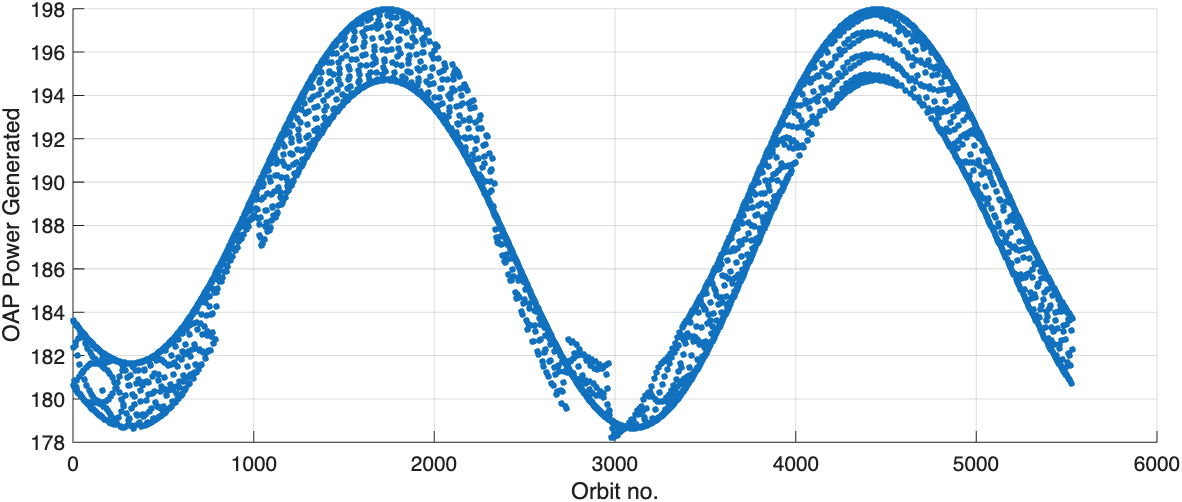
\includegraphics[width=0.7\textwidth]{figures/science_mode_power_generation.png}
    \caption{Power Generation Analysis in Science Mode}
    \label{fig:powergen}
\end{figure}

The power generation for the SA was determined to be $196\,\mathrm{W}$ in science mode using \autoref{eq:gen}. 

\begin{equation}
P_{gen} = \frac{\frac{P_eT_e}{X_e}+\frac{P_dT_d}{X_d}}{T_d}
\label{eq:gen}
\end{equation}

The target EOL specific power was determined to be $359\,\mathrm{W\,m^{-2}}$ using \autoref{eq:peol} at the worst-case solar angle incidence of $24^\circ$. 

\begin{equation}
P_{s_{eol}} = H_0*\eta_{cell}*cos(\beta)*\lambda_{cell}
\label{eq:peol}
\end{equation}

As such, the ideal SA area was determined to be 0.55m$^2$. However, in order to ensure that the power system can support the spacecraft in case of deployment failure a 1.5 safety factor was applied to this value, with a further 10\% margin covering cell shadowing and temperature variation. This led to an area of $0.91\,\mathrm{m^{-2}}$, which roughly equated to the area of three body panels. To ensure compatibility with the PCDU, the 242 main array cells were arranged in an 11s22p configuration, generating a maximum nominal voltage of $29.5\,\mathrm{V}$.


\subsubsection{Battery}

Batteries are necessary for power during eclipse, LEOP, decommissioning and the Collision Avoidance mode. The ideal battery capacity was sized using \autoref{eq:bat} to provide sufficient power to complete the deorbit burn in full eclipse; it was determined to be 452Wh. 

\begin{equation}
C_{bat} = \frac{P_eT_e}{DoD*N*n}
\label{eq:bat}
\end{equation}

Due to COTS availability, a $432\,\mathrm{Wh}$ battery pack from MP space was selected \cite{MPSpacePack2_2024}, which is less than the $452\,\mathrm{Wh}$ calculated above. Therefore to meet the energy requirement the battery will have to exceed $30\%$ DoD in some modes. Though this is unfavourable for battery lifetime, it is only needed during deorbit. Additionally, this battery provides a good compromise between performance (in nominal operations) and sufficient redundancy. Even in the case of 2 parallel string failing, the 8s3p configuration of the battery provides redundancy with a $15\%$ capacity margin during science mode. In the case of such a failure, the science and decomissioning burn must be sustained with a higher DoD. The battery has a nominal voltage of $28.8\,\mathrm{V}$, making it compatible with the PCDU and the system's power demands. At $5\,\mathrm{A}$ and from a $30\%$ DoD, the SA fully charges the battery within 57 minutes of sunlight.

\subsubsection{Power Distribution and Regulation}

The selection of electrical interfaces was driven by the input voltages of the platform and payload. A nominal $28\,\mathrm{V}$ unregulated bus was selected alongside three regulated voltage rails of $3.3$, $5$, and $12$ volts. To control platform power, maximum power point tracking (MPPT) was chosen over direct energy transfer. Unlike the latter, MPPT can modulate the amount of power generated, suiting it to the variation in power across different modes.

A pair of Bradford Space SuperNova PCDUs \cite{BradfordSupernova2024} were chosen to condition, regulate, and distribute the power as well as manage the charging and discharging of the batteries. The secondary, hot redundant, cross-strapped PCDU was incorporated given the power system’s indispensability to the mission’s success. The PCDU will operate the MPPT system at an electrical efficiency of $95\%$. It communicates with the OBC and propulsion system, sending telemetry data and thruster valves signals, respectively. A power draw analysis was also conducted to ensure that the current managed by the PCDU lies within its rated range. The total current of $27.9\,\mathrm{A}$ lies within the maximum of $50\,\mathrm{A}$, however, the $12\,\mathrm{V}$ and $28\,\mathrm{V}$ would exceed the rated current if all components were to operate at 100\% load. However, due to a conflict between the payload's and AOCS' peak operation, this would never occur. Therefore, the system is suitable for the mission. The complete analysis is available in \autoref{tab:power_draw} in the Appendix.

Remove before flight and separation switches were also incorporated within the architecture upstream of the PCDUs. The former maintains safety during ground handling of the spacecraft, and the latter ensures that power is provided to other subsystems only after launch vehicle separation.

\subsection{Thermal}
A TMS is crucial in providing a safe operating temperature range for the spacecraft's constituent components.  The key requirements driving the subsystem design were (THM-REQ-011) and (PLT-REQ-072). Given the effect of thermal coatings spacecraft’s radiation protection, the customer radiation requirements (SFG-REQ-120 and SFG-REQ-130) were also addressed within the thermal subsystem.
g
\subsubsection{Thermal Environment}
Whether operating or idle, every component has to be kept within a safe temperature range. The temperature range designed for nominal operations is between $0-40^\circ\,\mathrm{C}$, due the pressure sensor temperature limits, as can be seen in \autoref{tab:temperature}. Although the minimum operational temperature of the propulsion system components were higher at between $4-10^\circ\,\mathrm{C}$, their infrequent use warranted taking their idle temperature for the design case. 

A simple model based on the Thermal Balance Equation was initially used to determine the steady hot and cold cases experienced during Science Mode. The former is taken from the sunlit period and the latter is modelled in the eclipse. A summary of the findings can be found within \autoref{tab:thermal_cases}. Science mode was the selected design case, because of the transient nature of the other modes: internal dissipation is higher in Deorbit/Decommisioning, and
the total solar power across the spacecraft area is greater during LEOP detumbling. 

\begin{table}[H]
\centering
\caption{Thermal Analysis Cases}
\label{tab:thermal_cases}
\begin{tabular}{lSS}
\toprule
\textbf{Parameter} & \textbf{Hot Case (Science/Sunlight)} & \textbf{Cold Case (Science/Eclipse)} \\
\midrule
$Q_{\text{solar}}$ [W] & 337 & 0 \\
$Q_{\text{albedo}}$ [W] & 74 & 0 \\
$Q_{\text{IR}}$ [W] & 70 & 70 \\
$Q_{\text{internal}}$ [W] & 49 & 49 \\
\midrule
\textbf{Temperature} [\si{\degreeCelsius}] & \textbf{44} & \textbf{-55} \\
\bottomrule
\end{tabular}
\end{table}

The calculations factored in the properties of the coatings used on the spacecraft, as well as the view factors experienced for each of the heat inputs. Solar heat inputs were modelled on the +Y face, albedo inputs on the -Y face, and the IR inputs on the Y side facing the Earth. With the lunar albedo view factor being quite low at $0.00002$, this heat input was deemed as negligible and not included in the model. The emissivity values were taken as an average of the individual components and coatings covering the satellite’s external surface. 

This initial model was refined in MATLAB to account for the spacecraft’s transient response to the changes in temperature between sunlight and eclipse periods. It returns a better approximation of the thermal range experienced by the internal components. Since neither the material composition nor the thermal properties of individual components were available, the lumped mass model was extended to a one-node dynamic one. The specific heat capacity was assumed to be $900\,\mathrm{J\,kg}^{-1}\,\mathrm{K}^{-1}$ providing a balance between the metallic and composite mass fractions of the spacecraft. \autoref{fig:transientthermal} confirms thermal compliance, with an internal temperature range o $11-26^\circ\,\mathrm{C}$.

\begin{figure}[H]
    \centering
    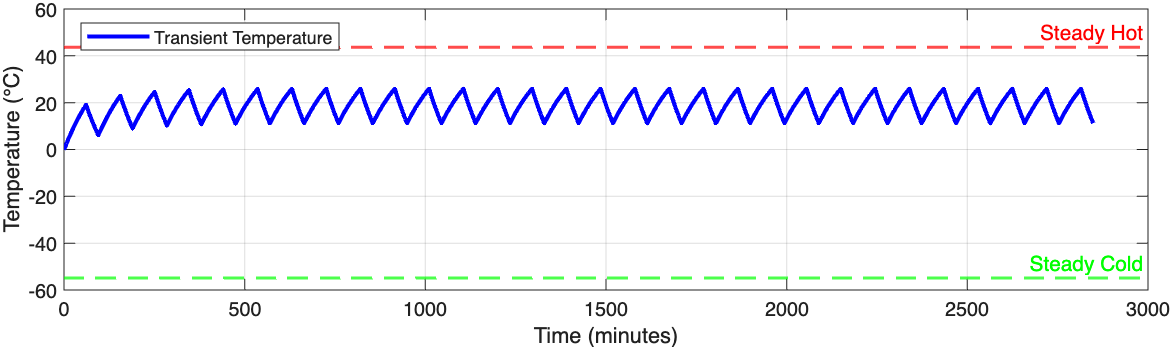
\includegraphics[width=0.7\textwidth]{figures/transient_thermal_response.png}
    \caption{Transient Thermal Response of SCIPIO-1}
    \label{fig:transientthermal}
\end{figure}

\subsubsection{Radiation Analysis}
Having selected the thermal coatings and materials for the outer panels, a radiation study was conducted in the MULASSIS tool. The software does not model CFRP composites, so an approximation was made based on the constituent materials’ chemical composition. Only surfaces covered with silver-coated FEP were modelled, since the Kapton-coated faces were largely covered with solar cells. The results of the analysis are available in \autoref{fig:radiation}, with it confirming that the configuration will reduce the TID on the internal components to $\approx3.5\,\mathrm{krad}$ over the mission’s 2-year duration, with trapped electrons contributing the highest dosage. Atomic oxygen deterioration will be mitigated by the \ce{SiO2} coating on the Kapton film. 

\begin{figure}[H]
    \centering
    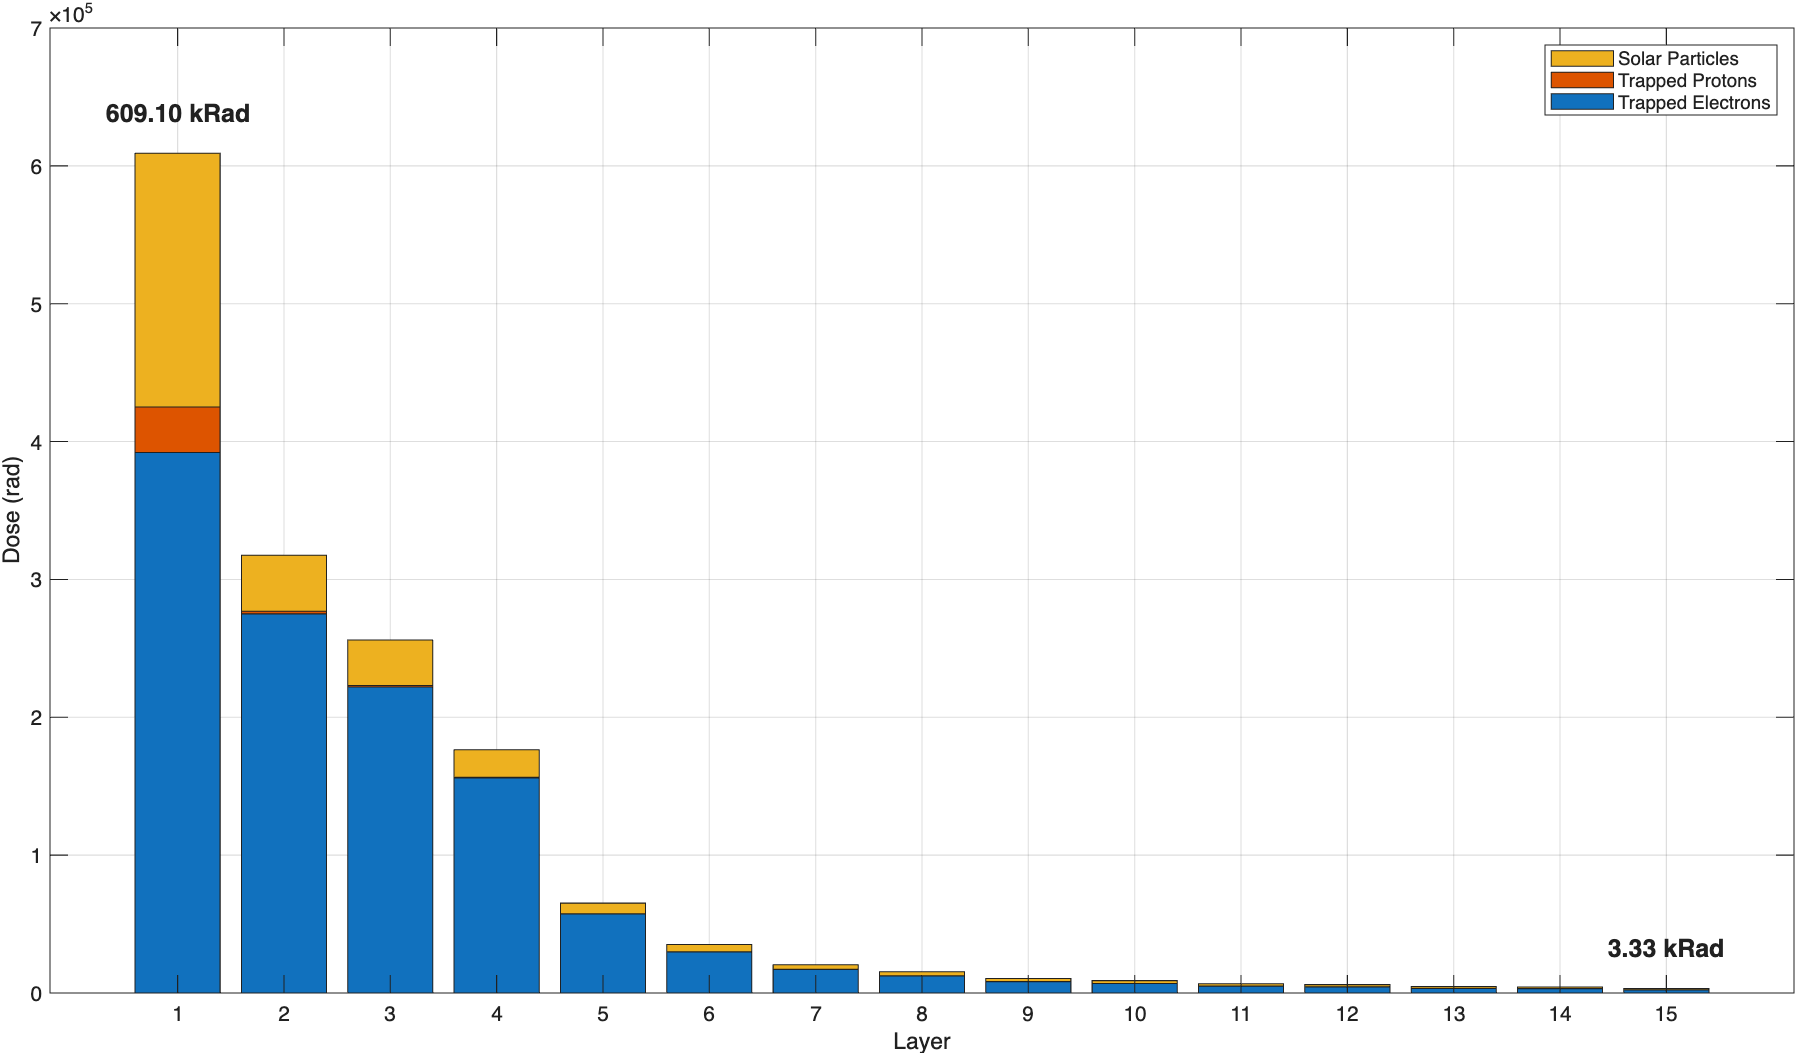
\includegraphics[width=0.7\textwidth]{figures/external_structure_radiation_protection.png}
    \caption{Radiation Protection (by layer) of the SCIPIO-1 External Structure}
    \label{fig:radiation}
\end{figure}
 
% ---------------------------------------------------------------------------
% ACKNOWLEDGMENT
% ---------------------------------------------------------------------------
\newpage


\section*{Acknowledgment}
\addcontentsline{toc}{section}{Acknowledgment}
We would like to extend our gratitude towards our supervisors Dr. Yusuf Açar and Ragnar Birgisson, who have helped us extensively throughout the design process with project vision and technical detail.

% ---------------------------------------------------------------------------
% BIBLIOGRAPHY
% ---------------------------------------------------------------------------
\bibliographystyle{ieeetr}
\bibliography{references}
\clearpage

% ---------------------------------------------------------------------------
% APPENDIX
% ---------------------------------------------------------------------------
\section{Appendix}

\subsection{Orbit Type Down-selection}
\label{subsec:orbit_downselection}
Having generated a list of orbit assessment criteria, a pairwise comparison was completed to assess their relative importance. The weightings from this were then fed into the following MCDA matrix. For each criterion, the orbits were ranked from 1 (worst) to 5 (best), though in many cases joint scores have been given. As can be seen in Table~\ref{tab:orbit_mcda}, a mid-morning sun-synchronous orbit was selected. 

\begin{table}[htbp]
\centering
\caption{Orbit Type MCDA (Note W.S. is the weighted score)}
\renewcommand{\arraystretch}{1.2}

\begin{tabularx}{\textwidth}{|l|c|c|c|c|c|c|c|c|c|c|c|}

\cline{1-12}
\textbf{Criteria} & \textbf{Weighting} &
\multicolumn{2}{c|}{\textbf{Polar}} &
\multicolumn{2}{c|}{\textbf{Equatorial}} &
\multicolumn{2}{c|}{\textbf{Molniya}} &
\multicolumn{2}{c|}{\textbf{Mid-morning SSO}} &
\multicolumn{2}{c|}{\textbf{Dawn–Dusk SSO}} \\
\cline{1-12}
& &
\textbf{Score} & \textbf{W.S.} &
\textbf{Score} & \textbf{W.S.} &
\textbf{Score} & \textbf{W.S.} &
\textbf{Score} & \textbf{W.S.} &
\textbf{Score} & \textbf{W.S.} \\
\cline{1-12}
\textbf{Power Generation}            & 0.18 & 3 & 0.5 & 3 & 0.5 & 4 & 0.7 & 3 & 0.5 & 5 & 0.9 \\
\cline{1-12}
\textbf{Thermal Stability}           & 0.09 & 3 & 0.3 & 3 & 0.3 & 4 & 0.4 & 3 & 0.3 & 5 & 0.5 \\
\cline{1-12}
\textbf{Comms Coverage}          & 0.16 & 3 & 0.5 & 5 & 0.8 & 4 & 0.6 & 3 & 0.5 & 3 & 0.5 \\
\cline{1-12}
\textbf{Perturbations}               & 0.11 & 4 & 0.4 & 4 & 0.4 & 5 & 0.5 & 4 & 0.4 & 4 & 0.4 \\
\cline{1-12}
\textbf{Deorbit lifetime}            & 0.07 & 5 & 0.4 & 5 & 0.4 & 1 & 0.1 & 5 & 0.4 & 5 & 0.4 \\
\cline{1-12}
\textbf{Radiation dose}              & 0.02 & 3 & 0.1 & 5 & 0.1 & 1 & 0.0 & 3 & 0.1 & 3 & 0.1 \\
\cline{1-12}
\textbf{Pressure}        & 0.02 & 3 & 0.1 & 3 & 0.1 & 5 & 0.1 & 3 & 0.1 & 3 & 0.1 \\
\cline{1-12}
\textbf{Accessibility}         & 0.34 & 3 & 1.0 & 2 & 0.7 & 1 & 0.3 & 5 & 1.7 & 3 & 1.0 \\
\cline{1-12}
\textbf{Total} & -- &
-- & \textbf{3.3} &
-- & \textbf{3.3} &
-- & \textbf{2.8} &
-- & \cellcolor{yellow!30}\textbf{3.9} &
-- & \textbf{3.8} \\
\cline{1-12}
\end{tabularx}
\label{tab:orbit_mcda}
\end{table}

\subsection{Product Breakdown Structure}
\label{sub:scipio_pbs}
\begin{figure}[H]
    \centering
    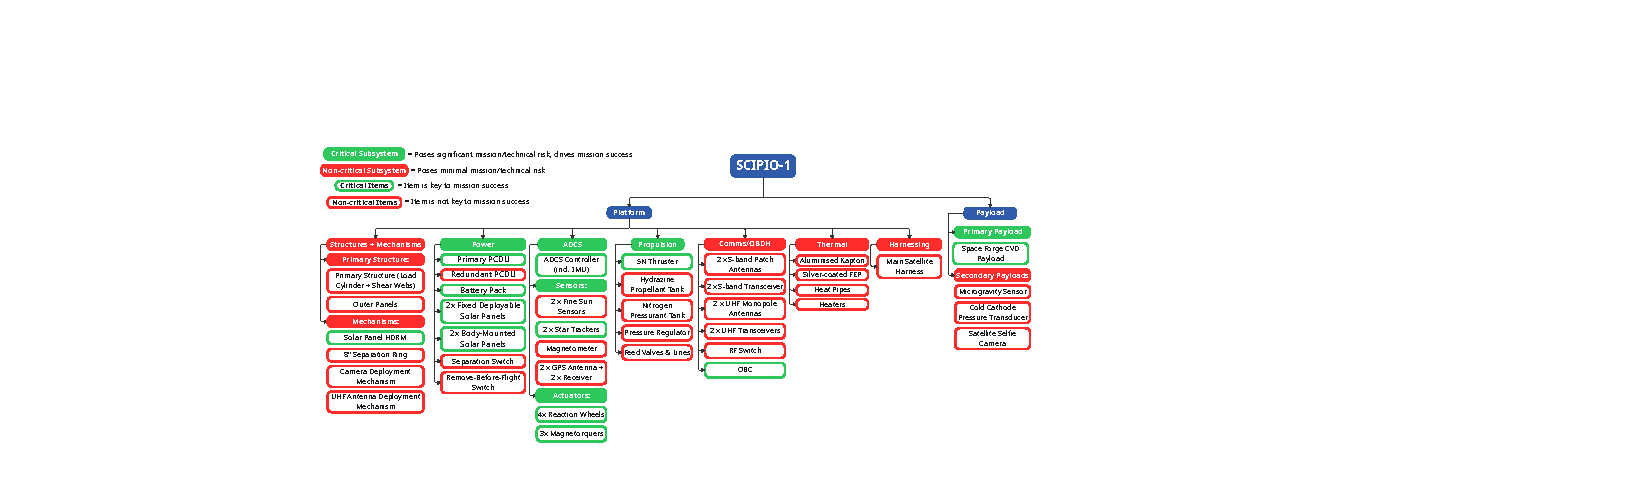
\includegraphics[width=0.9\linewidth]{figures/space_segment_product_breakdown.pdf}
    \caption{SCIPIO-1 Space Segment Product Breakdown Structure}
    \label{fig:scipio_pbs}
\end{figure}

\subsection{Full Requirements Verification}
\label{subsec:reqs_verif_appendix}
\begin{table}[H]
\centering
\caption{Full Customer Requirements Verification Matrix}
\label{tab:verif_mat_full}
\begin{tabularx}{\textwidth}{l c c X}
\toprule
\textbf{Req. ID} & \textbf{Compliance} & \textbf{Type} & \textbf{Evidence}\\
\midrule
SFG-REQ-010 & Yes & \textbf{A} & Overarching mission requirement. Compliance is predicted based on balanced budgets, mission lifetime analysis and use of heritage components.\\
SFG-REQ-020 & Yes & \textbf{D} & Inspection of CAD shows the satellite fits in the required envelope. \\
SFG-REQ-030 & Yes & \textbf{D/A} & All derived launch vehicle compatibility requirements have been met (XXX-REQ-031 to XXX-REQ-039). \\
SFG-REQ-040 & Partial & \textbf{D/A} & Satellite fits within the Ariane Half Plate volume envelope and can withstand launch loads. However, the natural frequency of the structure is incompatible with the launcher. \\
SFG-REQ-050 & Yes & \textbf{D/A} & Satellite fits within the Electron Shared volume envelope and test load cases for Falcon 9 exceed those of Electron. \\
SFG-REQ-060 & Yes & \textbf{A} & Itemised mass budget shows the mass is within the mass limits.\\
SFG-REQ-070 & Yes & \textbf{D/A} & All payload accommodation requirements have been met, including the derived requirements XXX-REQ-071 to XXX-REQ-077 \\
SFG-REQ-080 & Yes & \textbf{D/A} & The structure features multiple mounting points which have been verified to withstand the $40\,\mathrm{kg}$ satellite mass via hand calculation. \\
SFG-REQ-090 & Yes & \text{A} & In a dead on release scenario (random tumble, solar panels stowed), DRAMA predicts deorbit within $6.3$ to $8.0$ years with a $50\%$ confidence interval.\\
SFG-REQ-100 & Yes & \textbf{D} & There is no planned jettison of any satellite components during operation. \\
SFG-REQ-110 & No & \textbf{A} & DRAMA Demisability Analysis found that the composite pressurant tank will not burn up in orbit.\\
SFG-REQ-120 & Yes & \textbf{A} & MULASSIS tool was used to show that satellite structure is able to reduce TID to below $3.5\,\mathrm{krad}$ within the structure. \\
SFG-REQ-130 & Yes & \textbf{A} & As above, and external components (sun sensors, star trackers, selfie camera) are all rated to withstand $>16\,\mathrm{krad}$ of radiation. \\
SFG-REQ-140 & Yes & \textbf{D} & Inspection of the CAD shows the microgravity sensor within $100\,\mathrm{mm}$ of the payload. \\
SFG-REQ-150 & Yes & \textbf{A} & AOCS simulations show that magnetorquers are capable of maintaining payload accelerations below $10^{-4}\,\mathrm{g}$ during payload operations. \\
SFG-REQ-160 & Yes & \textbf{D} & Inspection of the CAD shows the pressure sensor within $100\,\mathrm{mm}$ of the payload. \\
SFG-REQ-170 & Yes & \textbf{A} & Pressure does not exceed $1\,\mathrm{mPa}$, even in worst case conditions (design altitude $-15\,\mathrm{km}$, ECSS “High” Solar and Geomagnetic Activity)\\
SFG-REQ-180 & Yes & \textbf{D} & CONOPS features a defined safe mode in which the satellite is sun-pointing. \\
SFG-REQ-190 & Yes & \textbf{D} & Selected GNSS receiver has position knowledge of $<10\,\mathrm{m}$ and CubeADCS features an IMU for velocity knowledge. \\
SFG-REQ-200 & Yes & \textbf{A} & Downlink budget for S-band accommodates the transmission of IMU and GNSS data in real-time \\
SFG-REQ-210 & Yes & \textbf{D} & Selected OBC features triple real-time clocks for timekeeping and redundancy.\\
SFG-REQ-220 & Yes & \textbf{A} & AOCS simulations show detumbling within 3 minutes using reaction wheels.\\
SFG-REQ-230 & Yes & \textbf{D} & Inspection of CAD shows the camera is mounted to include the Earth and Satellite in FOV \\
SFG-REQ-240 & Yes & \textbf{A} & Power budget shows margin in most modes, with batteries sized to handle the eclipse periods and deorbit burn. \\
SFG-REQ-250 & Yes & \textbf{D} & Satellite features full duplex S-band communications, supplemented by half duplex UHF comms \\
SFG-REQ-260 & Yes & \textbf{A} & STK access analysis indicates average pass lengths of 338s (6 min 38s) for UHF \\
SFG-REQ-270 & Yes & \textbf{D} & The UHF transceiver is capable of receiving 9600 Bps, whilst the S-band transceiver can receive 64 kBps thus both are capable of receiving 1 payload telecommand per second. \\
SFG-REQ-280 & Yes & \textbf{A} & Data budget shows downlink potential per day exceeds daily generation. Over S-band, an estimated 3 hours of platform data can be downlinked in a single average pass, whilst in RDT mode, the value rises to over 21 hours.\\
SFG-REQ-290 & Yes & \textbf{A} & STK access analysis shows a maximum gap between passes of 84.6 minutes over UHF using the Terran Network \\
SFG-REQ-300 & Yes & \textbf{A} & The data budget shows that daily downlink potential exceeds data generation per day. \\
SFG-REQ-310 & Yes & \textbf{A} & STK analysis shows a maximum gap between passes of 84.6 minutes over UHF using the Terran Network. Data budget shows downlink potential exceeds size of critical TM packet \\
SFG-REQ-320 & Yes & \textbf{D} & Satellite is equipped with star trackers to enable inertial pointing in Science Mode. \\
SFG-REQ-330 & Yes & \textbf{A} & The data budget accounts for the transmission of 1 payload photo per day, exceeding payload's photo capture frequency of 1 every 5 days \\
SFG-REQ-340 & Yes & \textbf{D} & Verify by inspection of the CAD \\
SFG-REQ-350 & Yes & \textbf{D} & Verify by inspection of the CAD \\

\bottomrule
\end{tabularx}
\end{table}


\begin{table}[H]
\centering
\caption{SerenSpace Derived Requirements Verification Matrix}
\label{tab:SSReqs_VCM}
\begin{tabularx}{\textwidth}{l c c X}
\toprule
\textbf{Requirement ID} & \textbf{Compliance} & \textbf{Type} & \textbf{Evidence}\\
\midrule
THM-REQ-011 & Yes & \textbf{A} & Single node thermal model suggests an achieved temperature range of $8^\circ$\.C to $22^\circ$\,C.  \\
SAT-REQ-031 & Yes & \textbf{D} & Inspection of CAD shows the satellite fits within the required envelope. \\
SAT-REQ-032 & Yes & \textbf{A} & Weighted CAD model indicates that the satellite's centre of mass lies within 350\,mm of the payload origin. \\
SAT-REQ-033 & Yes & \textbf{A} & The satellite has been tested to withstand all limit launch loads. \\
SAT-REQ-034 & Yes & \textbf{D} & The satellite has been designed to accommodate an MLB Mk2 8" Separation Ring  \\
PRP-REQ-035 & Yes & \textbf{D} & All selected pressure vessels comply with the necessary standards \\
PRP-REQ-036 & Yes & \textbf{D} & P\&ID demonstrates presence of burst disks along pressurised lines. \\
PRP-REQ-037 & Yes & \textbf{D} & All selected  valves, fittings and regulators are compliant according to supplier datasheets.  \\
PRP-REQ-038 & Yes & \textbf{D} & Latching solenoid valves have been included in series on pressure run lines. \\
MIS-REQ-039 & Yes & \textbf{A} & At the nominal 520\,km altitude, DRAMA predicts natural deorbit within 6.7 years, whilst STK predicts 6.5 years. Thus the satellite can deorbit within 5 years of its 2 year mission life naturally, even in the event of propulsion failure.  \\
PLM-REQ-071 & Partial & \textbf{D} & The satellite designates the required volume, though mounting holes have not been modelled. \\
PLT-REQ-072 & Yes & \textbf{A} & The calculated hot case and cold case temperatures fall within the payloads operating limits. \\
PLP-REQ-073 & Yes & \textbf{A} & The power budget features a 10\,W constant draw from the payload in Science Mode \\
PLP-REQ-074 & Yes & \textbf{A} & The power budget features an 80\,W spike lasting for 10 minutes each day from the payload \\
PLP-REQ-075 & Yes & \textbf{A} & The power budget features a 1\,W constant draw from the payload in Commissioning, Safe Mode, Collision Avoidance Mode and Rapid Data Transfer Mode. \\
PLO-REQ-076 & Yes & \textbf{D} & The satellite is designed to be operational for 2 years, with the payload operational by default. \\
PLO-REQ-077 & Yes & \textbf{D} & CONOPS definition features a minimum of 2 weeks in Commissioning, with the satellite only entering nominal operations post IOCR\label(nom:iocr) \\
AOC-REQ-001 & Yes & \textbf{A} & The reaction wheels are capable of counteracting $0.1^\circ$ of thruster misalignment with a considerable margin of $291\%$ \\
\bottomrule
\end{tabularx}
\end{table}

\begin{table}[htbp]
\centering
\caption{Final Verification Plan for Customer Requirements}
\label{tab:Final_Verif_Plan}
\begin{tabularx}{\textwidth}{l c X c}
\toprule
\textbf{Req. ID} & \textbf{Type} & \textbf{Plan} & \textbf{Final Verification Point}\\
\midrule
SFG-REQ-010 & \textbf{T} & Initial verification during FlatSat functional testing, with final verification during System End-to-End Testing (SEET)\label{nom:seet}. & SEET \\
SFG-REQ-020 & \textbf{I} & Perform mechanical inspection of the integrated satellite. & AIT \\
SFG-REQ-030 & \textbf{I/T} & Perform quasistatic/vibration/shock testing testing on qualification model of the satellite. Perform acceptance testing on flight model. & Launch Certification\\
SFG-REQ-040 & \textbf{I/T} & " & Launch Certification \\
SFG-REQ-050 & \textbf{I/T} & " & Launch Certification \\
SFG-REQ-060 & \textbf{I} & Use calibrated scales to weigh the integrated satellite & AIT \\
SFG-REQ-070 & \textbf{T} & Carry out all required interface tests, functional tests and SEET & SEET \\
SFG-REQ-080 & \textbf{T} & Test the mounting points using a test load prior to mounting the satellite from them. & AIT \\
SFG-REQ-110 & \textbf{A} & Repeat SARA\label{nom:sara} testing following the next design iteration & CDR\label{nom:cdr} \\
SFG-REQ-160 & \textbf{T} & As the pressure sensor is not space-rated, it will require full qualification testing, most notably Thermal Vacuum (TVAC) Testing & TVAC \\ 
SFG-REQ-180 & \textbf{T} & Verify by testing safe mode functionality in system-level functional testing & Functional Testing\\
SFG-REQ-200 & \textbf{T} & Verify by real-time telemetry function during functional testing & Functional Testing \\
SFG-REQ-230 & \textbf{T} & Test camera operation during functional testing & Functional Testing \\
SFG-REQ-270 & \textbf{T} & Test receiver functionality during unit, subsystem and system-level functional testing & Functional Testing\\
SFG-REQ-330 & \textbf{T} & Test image transmission functionality during system-level functional testing & Functional Testing \\

\bottomrule
\end{tabularx}
\end{table}

\clearpage

\subsection{Full Mass Budget}

\begin{table}[H]
\centering
\caption{Subsystem Mass Budget}
\begin{sideways}
\scriptsize
\begin{tabularx}{0.9\textheight}{l X c c c c c}
\toprule
\textbf{Subsystem} & \textbf{Item} & \textbf{Unit Mass (kg)} & \textbf{Qty} & \textbf{\% Allocation} & \textbf{Equip. Margin (\%)} & \textbf{Mass w/ Margin (kg)} \\
\midrule

Comms/OBDH  & OBC & 0.7 & 1 & 1.86 & 5 & 0.74 \\
            & Spacemanic MURGAS UHF Transceiver & 0.025 & 2 & 0.13 & 5 & 0.05 \\
            & IQ Spacecom Slink-Phy S-band Transceiver & 0.42 & 1 & 1.11 & 5 & 0.44 \\
            & Spacemanic SAM UHF Antenna Module & 0.055 & 2 & 0.29 & 5 & 0.12 \\
            & Anywaves S-band Patch Antenna & 0.136 & 2 & 0.72 & 5 & 0.29 \\
\midrule
Thermal     & Heat Pipes & 1 & 1 & 2.65 & 20 & 1.20 \\
            & Heaters & 0.0028 & 8 & 0.06 & 5 & 0.02 \\
            & Thermistors & 0.00007 & 30 & 0.01 & 5 & 0.00 \\
\midrule
Power       & Battery Packs & 2.33 & 1 & 6.18 & 5 & 2.45 \\
            & PCDU & 1 & 2 & 5.30 & 5 & 2.10 \\
            & Solar Cells & 0.0024 & 312 & 1.99 & 5 & 0.79 \\
\midrule
Payload     & Space Forge CVD Payload & 3.4 & 1 & 9.01 & 5 & 3.57 \\
            & Silicon Sensing CAS290 Gravity Sensor & 0.0006 & 1 & 0.00 & 5 & 0.00 \\
            & MKS 971B UniMag Cold Cathod Pressure Transducer & 0.36 & 1 & 0.95 & 20 & 0.43 \\
            & Infinity Avionics LEO2MP & 0.065 & 1 & 0.17 & 5 & 0.07 \\
\midrule
AOCS        & CubeSpace CR0100 Magnetorquers & 0.272 & 3 & 2.16 & 5 & 0.86 \\
            & CubeSpace CW1200 Damped Reaction Wheels Assembly (x4) & 2.422 & 1 & 6.42 & 5 & 2.54 \\
            & CubeADCS & 0.25 & 1 & 0.66 & 5 & 0.26 \\
            & CubeStar Gen 2 & 0.047 & 2 & 0.25 & 5 & 0.10 \\
            & CubeSense Sun & 0.015 & 2 & 0.08 & 5 & 0.03 \\
            & CubeMag Gen 2 (Compact) & 0.006 & 1 & 0.02 & 5 & 0.01 \\
            & GPS Antenna & 0.089 & 2 & 0.47 & 5 & 0.19 \\
            & GPS Receiver & 0.024 & 2 & 0.13 & 5 & 0.05 \\
\midrule
Propulsion  & Hydrazine Propellant & 2.6 & 1 & 6.89 & 10 & 2.86 \\
            & Nitrogen Pressurant & 0.12 & 1 & 0.32 & 10 & 0.13 \\
            & RAFAEL 5N Thruster & 0.31 & 1 & 0.82 & 5 & 0.33 \\
            & PBT-3 Hydrazine Bladder Tank & 1.75 & 1 & 4.64 & 5 & 1.84 \\
            & ARDE-4821 Nitrogen Tank & 1.23 & 1 & 3.25 & 5 & 1.29 \\
            & Propulsion system shape memory alloy valve & 0.16 & 2 & 0.85 & 5 & 0.34 \\
            & RV29 Pressure regulator & 1.452 & 1 & 3.85 & 5 & 1.52 \\
            & High Pressure Gas fill valve & 0.113 & 1 & 0.30 & 5 & 0.12 \\
            & Propulsion Fill and Drain Valve & 0.08 & 1 & 0.21 & 5 & 0.08 \\
            & ML 2000 Series mini Pressure Transducer & 0.54 & 3 & 4.29 & 5 & 1.70 \\
            & Latching Solenoid valve & 0.37 & 2 & 1.96 & 5 & 0.78 \\
\midrule
Harness     & Harnessing & 1.6 & 1 & 4.24 & 0 & 1.60 \\
\midrule
Structure   & Structure & 7.102 & 1 & 18.83 & 20 & 8.52 \\
            & Mounting Structures & 1 & 1 & 2.65 & 5 & 1.05 \\
            & Solar Panels & 0.44 & 2 & 2.33 & 20 & 1.06 \\
            & MLB Separation Interface & 1.48 & 1 & 3.92 & 5 & 1.55 \\
\midrule
\textbf{Total} & & \textbf{32.97} &  & \textbf{100.00} &  & \textbf{41.06} \\
\bottomrule
\end{tabularx}
\end{sideways}
\end{table}

\FloatBarrier

\clearpage
\subsection{Full Link Margin}
\begin{table}[H]
\centering
\caption{Full Link Budget}
\label{tab:fedr_link_budget}

\begin{sideways}
\footnotesize 
\setlength{\tabcolsep}{4pt}

\begin{tabular}{|l|c|c||c|c|c|c|c|c|}
\hline
\multicolumn{3}{|c||}{\textbf{Link Budget Properties}} & \multicolumn{3}{|c|}{\textbf{Downlink}} & \multicolumn{3}{|c|}{\textbf{Uplink}} \\
\cline{1-9}
\textbf{Variable} & \textbf{Abbreviation} & \textbf{Equation} & \textbf{UHF} & \multicolumn{2}{|c|}{\textbf{S-Band}} & \textbf{UHF } & \multicolumn{2}{|c|}{\textbf{S-Band}} \\
\hline
\hline

% --- PROPERTIES SECTION ---
\multicolumn{9}{|l|}{\textbf{Properties}} \\
\hline
Function & N/A & N/A & Critical & Nominal & RDT & Critical & Nominal & RDT  \\
Frequenecy ($\mathrm{GHz}$)& $\lambda$ & $\lambda = (3\cdot10^8)/F_t$ & 0.400 & 2.250 & 2.250 & 0.400 & 2.075 & 2.075 \\
Distance to ground ($\mathrm{km}$) & $d$ & N/A & 3000 & 3000 & 2000 & 3000 & 3000 & 2000  \\
Rate ($\mathrm{kbps}$) & $R$ & N/A & 38.6 & 600 & 4000 & 9.6 & 64.0 & 64.0  \\
Modulation & N/A & N/A & GMSK & QPSK & QPSK & GMSK & BPSK & BPSK \\
\hline
\hline

% --- TRANSMITTER LOSSES/GAINS SECTION ---
\multicolumn{9}{|l|}{\textbf{Transmitter losses/gains}} \\
\hline
Bit Rate loss & $L_R$ & $10\log_{10}(R)$ & 45.9 & 57.8 & 66.0 & 39.8 & 48.1 & 48.1\\
Transmit Power ($\mathrm{dBm}$) & $P_t$ & N/A & 30.0 & 30.0 & 30.0 & 30.0 & 30.0 & 30.0 \\
Passive Loss ($\mathrm{dB}$) & $L_p$ & N/A & 2.0 & 2.0 & 2.0 & 2.0 & 2.0 & 2.0 \\
Transmit Antenna Gain ($\mathrm{dBiC}$) & $G_t$ & N/A & 2.6 & 0.0 & 4.5 & 22.3 & 35.9 & 35.9  \\
EIRP ($\mathrm{dBm}$) & $EIRP$ & $EIRP = P_t-L_p+G_t$ & 30.6 & 28.0 & 32.5 & 50.3 & 63.9 & 63.9  \\
\hline
\hline

% --- TRANSMISSION LOSSES SECTION ---
\multicolumn{9}{|l|}{\textbf{Transmission losses}} \\
\hline
Path Loss ($\mathrm{dB}$) & $L_p$ & $L_P =20\log_{10}(4\pi d/\lambda)$ & 154.0 & 169.0 & 165.5 & 154.0 & 168.5 & 164.8  \\
Atmospheric Loss ($\mathrm{dB}$) & $L_a$ & N/A & 1.0 & 1.0 & 1.0 & 1.0 & 1.0 & 1.0 \\
\hline
\hline

% --- RECEIVER LOSSES/GAINS SECTION ---
\multicolumn{9}{|l|}{\textbf{Receiver losses/gains}} \\
\hline
Ground antenna efficiency & $\eta$ & N/A & N/A & 0.6 & 0.6 & N/A & N/A & N/A \\
Ground aperture & $A_g$ & N/A & N/A & 10.8 & 10.8 & N/A & N/A & N/A  \\
Ground Gain numerical & $G_{num}$ & $G_{num} = \eta \pi (R/\lambda)^2$ & N/A & 4560.1 & 4560.1 & N/A & N/A & N/A  \\
Ground Antenna Gain ($\mathrm{dBiC}$) & $G_g$ & $G_g = 10\log_{10}(G_{num})$ & 22.3 & 36.6 & 36.6 & 2.6 & 0.0 & 4.5  \\
Total Received Power (dBm) & $C$ & $C = EIRP+G_g-L_p-L_a$ & 102.1 & 105.4 & 97.4 & 102.1 & 105.4 & 97.4  \\
System Noise Density ($\mathrm{dBm/Hz}$) & $N_0$ & $N_0 = k \cdot T_s$ & 174.6 & 174.6 & 174.6 & 174.6 & 174.6 & 174.6 \\
Received $(Eb/N0)$ & $(Eb/N0)_{C}$ & $(Eb/N0)_{C} = C- N_0 - L_R$ & 26.6 & 11.4 & 11.2 & 32.7 & 21.2 & 29.2 \\
Required $(Eb/N0)$ & $(Eb/N0)_{Q}$ & N/A & 12.5 & 1.9 & 1.9 & 12.5 & 8.0 & 8.0  \\
Receiver System Loss & $L_R$ & N/A & 3.0 & 3.0 & 3.0 & 3.0 & 3.0 & 3.0 \\
\hline
\textbf{Link Margin (dB)} & \textbf{LM} &  $\mathbf{(Eb/N0)Rec - (Eb/N0)Req - L_R}$ & \textbf{11.1} & \textbf{6.5} & \textbf{6.3} & \textbf{17.2} & \textbf{10.2} & \textbf{18.2} \\
\hline
\end{tabular}
\end{sideways}
\end{table}

\FloatBarrier

\clearpage

% Preamble must include:
% \usepackage{rotating}
% \usepackage{float}
% \usepackage{placeins}

\clearpage
\subsection{Full Data Budget}
\label{sub:FULL_DATA_BUDGET}

\begin{table}[H]
\centering
\caption{Subsystem data generation under nominal and safe operations}
\label{tab:data_budget_nominal_orig}

\begin{sideways}
\footnotesize
\setlength{\tabcolsep}{4pt}
\begin{tabular}{ll|ll|ll|}
\cline{3-6}
\textbf{} & \textbf{} & \multicolumn{2}{l|}{\textbf{Data Rates (BPS)}} & \multicolumn{2}{l|}{\textbf{Data Generated (MB/day)}} \\ \hline
\multicolumn{1}{|l|}{\textbf{Subsystem}} & \textbf{Component} & \multicolumn{1}{l|}{\textbf{Nominal}} & \textbf{Safe mode} & \multicolumn{1}{l|}{\textbf{Nominal}} & \textbf{Safemode} \\ \hline

\multicolumn{1}{|l|}{\textbf{AOCS}} & \textbf{IMU} & \multicolumn{1}{l|}{4096} & 4096 & \multicolumn{1}{l|}{353.8944} & 353.8944 \\
\multicolumn{1}{|l|}{} & \textbf{Magnetometer} & \multicolumn{1}{l|}{409.6} & 409.6 & \multicolumn{1}{l|}{35.38944} & 35.38944 \\
\multicolumn{1}{|l|}{} & \textbf{Sun sensor} & \multicolumn{1}{l|}{2048} & 2048 & \multicolumn{1}{l|}{176.9472} & 176.9472 \\
\multicolumn{1}{|l|}{} & \textbf{Star tracker} & \multicolumn{1}{l|}{614.4} & 614.4 & \multicolumn{1}{l|}{53.08416} & 53.08416 \\
\multicolumn{1}{|l|}{} & \textbf{GPS} & \multicolumn{1}{l|}{1200} & 1200 & \multicolumn{1}{l|}{103.68} & 103.68 \\
\multicolumn{1}{|l|}{} & \textbf{Reaction Wheel} & \multicolumn{1}{l|}{2457.6} & 2457.6 & \multicolumn{1}{l|}{212.33664} & 212.33664 \\
\multicolumn{1}{|l|}{} & \textbf{Magnetorquer} & \multicolumn{1}{l|}{1228.8} & 1228.8 & \multicolumn{1}{l|}{106.16832} & 106.16832 \\
\multicolumn{1}{|l|}{} & \textbf{Thruster} & \multicolumn{1}{l|}{819.2} & 819.2 & \multicolumn{1}{l|}{70.77888} & 70.77888 \\

\multicolumn{1}{|l|}{\multirow{2}{*}{\textbf{Power}}} & \textbf{PCDU} & \multicolumn{1}{l|}{108} & 108 & \multicolumn{1}{l|}{9.3312} & 9.3312 \\
\multicolumn{1}{|l|}{} & \textbf{Battery} & \multicolumn{1}{l|}{150} & 150 & \multicolumn{1}{l|}{12.96} & 12.96 \\

\multicolumn{1}{|l|}{\multirow{3}{*}{\textbf{Propulsion}}} & \textbf{ML2000 Pressure Transducer (x3)} & \multicolumn{1}{l|}{24} & 24 & \multicolumn{1}{l|}{2.0736} & 2.0736 \\
\multicolumn{1}{|l|}{} & \textbf{Rafael Latching Solenoid Valve (x2)} & \multicolumn{1}{l|}{4} & 4 & \multicolumn{1}{l|}{0.3456} & 0.3456 \\
\multicolumn{1}{|l|}{} & \textbf{Rafael High pressure valve (x2)} & \multicolumn{1}{l|}{2} & 2 & \multicolumn{1}{l|}{0.1728} & 0.1728 \\

\multicolumn{1}{|l|}{\textbf{Thermal}} & \textbf{Thermisor (x30)} & \multicolumn{1}{l|}{32} & 32 & \multicolumn{1}{l|}{2.7648} & 2.7648 \\

\multicolumn{1}{|l|}{\multirow{3}{*}{\textbf{Satellite}}} & \textbf{Pressure sensor} & \multicolumn{1}{l|}{8} & 8 & \multicolumn{1}{l|}{0.6912} & 0.6912 \\
\multicolumn{1}{|l|}{} & \textbf{Gravity sensor} & \multicolumn{1}{l|}{24} & 24 & \multicolumn{1}{l|}{2.0736} & 2.0736 \\
\multicolumn{1}{|l|}{} & \textbf{Camera} & \multicolumn{1}{l|}{0} & 0 & \multicolumn{1}{l|}{4} & 0 \\ \hline

\multicolumn{1}{|l|}{\textbf{Platform Subtotal}} &  & \multicolumn{1}{l|}{13225.6} & 13225.6 & \multicolumn{1}{l|}{1146.69184} & 1142.69184 \\ \hline

\multicolumn{1}{|l|}{\multirow{3}{*}{\textbf{Payload}}} & \textbf{Scientific Data} & \multicolumn{1}{l|}{128} & 32 & \multicolumn{1}{l|}{11.0592} & 2.7648 \\
\multicolumn{1}{|l|}{} & \textbf{Critical Telemetry} & \multicolumn{1}{l|}{0} & 0 & \multicolumn{1}{l|}{9.60E-05} & 9.60E-05 \\
\multicolumn{1}{|l|}{} & \textbf{Imaging} & \multicolumn{1}{l|}{0} & 0 & \multicolumn{1}{l|}{3.00E-02} & 0 \\ \hline

\multicolumn{2}{|l|}{\textbf{Payload Subtotal}} & \multicolumn{1}{l|}{128} & 32 & \multicolumn{1}{l|}{11.089296} & 2.764896 \\ \hline

\multicolumn{2}{|l|}{\textbf{Total}} & \multicolumn{1}{l|}{13353.6} & 13257.6 & \multicolumn{1}{l|}{1157.781136} & 1145.456736 \\ \hline

\end{tabular}
\end{sideways}
\end{table}

\clearpage

\subsection{Power Draw Analysis}

\begin{table}[H]
\centering
\caption{PDCU Current Draw}
\label{tab:power_draw}
\begin{tabular}{lc}
\toprule
\textbf{Voltage Rail} & \textbf{Peak Current [A]} \\
\midrule
Max System Current & 50.0 \\
Max Rail Current & 10.0 \\
\midrule
3.3 V & 0.8 \\
5 V & 4.0 \\
12 V & 12.5 \\
28 V & 10.6 \\
\midrule
\textbf{Total Current} & \textbf{27.9} \\
\bottomrule
\end{tabular}
\end{table}
\subsection{Complete Ground Station Network}
\begin{figure}[H]
    \centering
    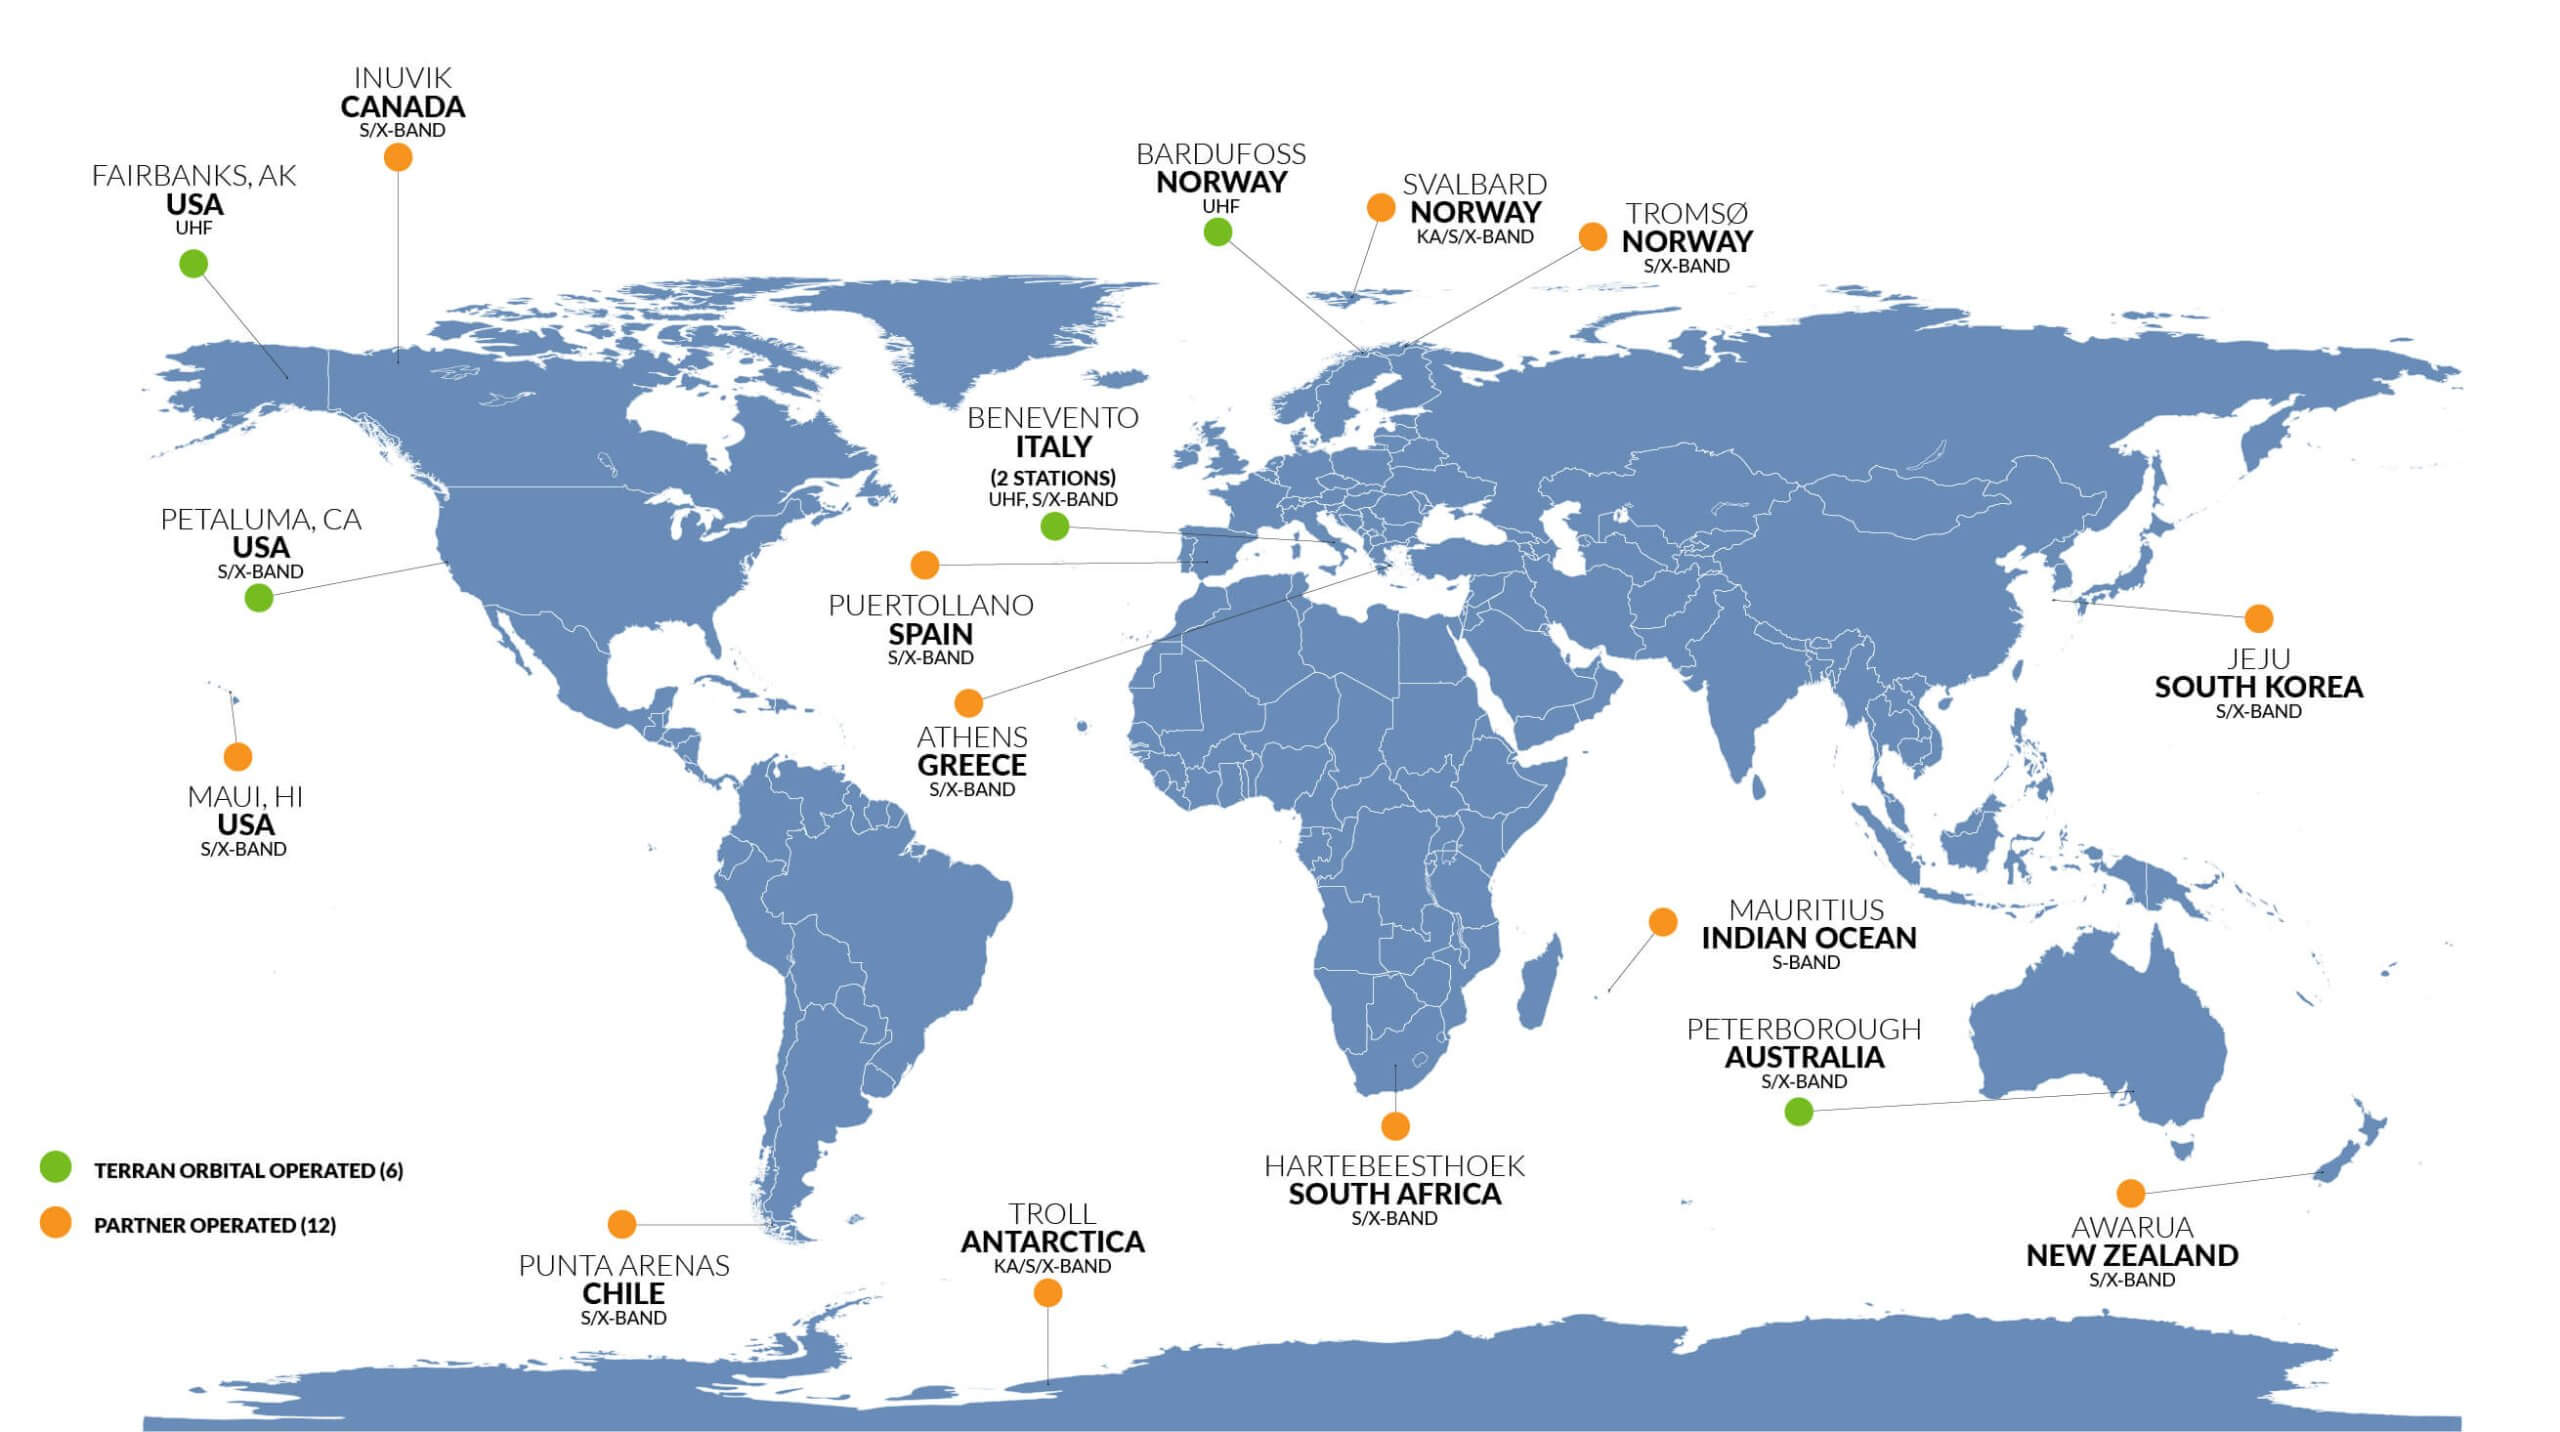
\includegraphics[width=0.9\linewidth]{figures/terran_ground_station_network.jpg}
    \caption{Terran Network}
    \label{fig:Terran}
\end{figure}
\clearpage
\begin{landscape}
\subsection{Actuator Down-Selection}

% ---- ACTUATOR ----
\begin{table}[H]
\centering
\caption{Actuator MCDA Matrix}
\label{tab:actuator_downselection}
\setlength{\tabcolsep}{3pt}
\resizebox{1.2\textwidth}{!}{%
\begin{tabular}{p{3.2cm} *{11}{c}}
\toprule
\multirow{2}{*}{Criteria} & 
\multirow{2}{*}{Weightings} & 
\multicolumn{2}{c}{\cellcolor{yellow!25}MTQs} & 
\multicolumn{2}{c}{\cellcolor{yellow!25}Reaction Wheels} & 
\multicolumn{2}{c}{CMGs} & 
\multicolumn{2}{c}{Passive Methods} & 
\multicolumn{2}{c}{Reaction Thrusters} \\
\cmidrule(lr){3-4} \cmidrule(lr){5-6} \cmidrule(lr){7-8} \cmidrule(lr){9-10} \cmidrule(lr){11-12}
 & & score & \cellcolor{yellow!25}weighted & score & \cellcolor{yellow!25}weighted & score & weighted & score & weighted & score & weighted \\
\midrule
Torque authority / slew & 0.21 & 3 & \cellcolor{yellow!25}0.63 & 7 & \cellcolor{yellow!25}1.47 & 9 & 1.89 & 1 & 0.21 & 9 & 1.89 \\
Fine pointing \& bandwidth & 0.26 & 5 & \cellcolor{yellow!25}1.30 & 9 & \cellcolor{yellow!25}2.34 & 7 & 1.82 & 1 & 0.26 & 5 & 1.30 \\
Disturbance \& vibration & 0.15 & 9 & \cellcolor{yellow!25}1.35 & 3 & \cellcolor{yellow!25}0.45 & 1 & 0.15 & 9 & 1.35 & 3 & 0.45 \\
Power consumption & 0.08 & 9 & \cellcolor{yellow!25}0.72 & 5 & \cellcolor{yellow!25}0.40 & 3 & 0.24 & 9 & 0.72 & 5 & 0.40 \\
Mass / volume & 0.07 & 7 & \cellcolor{yellow!25}0.49 & 5 & \cellcolor{yellow!25}0.35 & 1 & 0.07 & 7 & 0.49 & 1 & 0.07 \\
Reliability \& lifetime & 0.15 & 9 & \cellcolor{yellow!25}1.35 & 5 & \cellcolor{yellow!25}0.75 & 3 & 0.45 & 9 & 1.35 & 3 & 0.45 \\
Operational complexity & 0.08 & 7 & \cellcolor{yellow!25}0.56 & 5 & \cellcolor{yellow!25}0.40 & 1 & 0.08 & 9 & 0.72 & 1 & 0.08 \\
\midrule
Total & 1.00 &  & \cellcolor{yellow!25}6.4 &  & \cellcolor{yellow!25}6.2 &  & 4.7 &  & 5.1 &  & 4.6 \\
\bottomrule
\end{tabular}}
\end{table}

% ---- SENSOR ----
\subsection{Sensor Down-Selection}
\begin{table}[H]
\centering
\caption{Sensor MCDA Matrix}
\label{tab:sensor_downselection}
\setlength{\tabcolsep}{3pt}
\renewcommand{\arraystretch}{1.15}
\resizebox{1.2\textwidth}{!}{%
\begin{tabular}{l *{15}{c}}
\toprule
\multirow{2}{*}{Criteria} &
\multirow{2}{*}{Weightings} &
\multicolumn{2}{c}{\cellcolor{yellow!25}Star Tracker} &
\multicolumn{2}{c}{\cellcolor{yellow!25}Fine Sun Sensor} &
\multicolumn{2}{c}{\cellcolor{yellow!25}Magnetometer} &
\multicolumn{2}{c}{\cellcolor{yellow!25}IMU} &
\multicolumn{2}{c}{\cellcolor{yellow!25}GNSS} &
\multicolumn{2}{c}{Coarse Sun Sensor} &
\multicolumn{2}{c}{Earth Horizon Sensor} \\
\cmidrule(lr){3-4}\cmidrule(lr){5-6}\cmidrule(lr){7-8}\cmidrule(lr){9-10}
\cmidrule(lr){11-12}\cmidrule(lr){13-14}\cmidrule(lr){15-16}
 & & score & \cellcolor{yellow!25}weighted & score & \cellcolor{yellow!25}weighted &
 score & \cellcolor{yellow!25}weighted & score & \cellcolor{yellow!25}weighted &
 score & \cellcolor{yellow!25}weighted & score & weighted & score & weighted \\
\midrule
Accuracy & 0.32
& 9 & \cellcolor{yellow!25}2.88
& 4 & \cellcolor{yellow!25}1.28
& 3 & \cellcolor{yellow!25}0.96
& 7 & \cellcolor{yellow!25}2.24
& 2 & \cellcolor{yellow!25}0.64
& 1 & 0.32
& 1 & 0.32 \\
Availability / FOV limits & 0.18
& 4 & \cellcolor{yellow!25}0.72
& 8 & \cellcolor{yellow!25}1.44
& 8 & \cellcolor{yellow!25}1.44
& 9 & \cellcolor{yellow!25}1.62
& 9 & \cellcolor{yellow!25}1.62
& 7 & 1.26
& 5 & 0.90 \\
Drift / stability & 0.15
& 9 & \cellcolor{yellow!25}1.35
& 3 & \cellcolor{yellow!25}0.45
& 3 & \cellcolor{yellow!25}0.45
& 4 & \cellcolor{yellow!25}0.60
& 2 & \cellcolor{yellow!25}0.30
& 1 & 0.15
& 1 & 0.15 \\
Power consumption & 0.10
& 5 & \cellcolor{yellow!25}0.50
& 9 & \cellcolor{yellow!25}0.90
& 9 & \cellcolor{yellow!25}0.90
& 4 & \cellcolor{yellow!25}0.40
& 4 & \cellcolor{yellow!25}0.40
& 9 & 0.90
& 7 & 0.70 \\
Robustness / simplicity & 0.15
& 6 & \cellcolor{yellow!25}0.90
& 8 & \cellcolor{yellow!25}1.20
& 7 & \cellcolor{yellow!25}1.05
& 5 & \cellcolor{yellow!25}0.75
& 7 & \cellcolor{yellow!25}1.05
& 9 & 1.35
& 8 & 1.20 \\
Operational flexibility & 0.10
& 8 & \cellcolor{yellow!25}0.80
& 5 & \cellcolor{yellow!25}0.50
& 5 & \cellcolor{yellow!25}0.50
& 9 & \cellcolor{yellow!25}0.90
& 6 & \cellcolor{yellow!25}0.60
& 2 & 0.20
& 2 & 0.20 \\
\midrule
Total & 1.00
&  & \cellcolor{yellow!25}7.15
&  & \cellcolor{yellow!25}5.77
&  & \cellcolor{yellow!25}5.30
&  & \cellcolor{yellow!25}6.51
&  & \cellcolor{yellow!25}4.61
&  & 4.28
&  & 3.52 \\
\bottomrule
\end{tabular}}
\end{table}
\end{landscape}
\clearpage

% ---- SOLAR CELL ----
\begin{landscape}
\begin{table}[H]
\centering
\caption{Solar Cell Technology MCDA}
\label{tab:cellmcda}
\setlength{\tabcolsep}{3pt}
\renewcommand{\arraystretch}{1.15}
\resizebox{1.2\textwidth}{!}{%
\begin{tabular}{l *{11}{c}}
\toprule
\multirow{2}{*}{Criteria} &
\multirow{2}{*}{Weightings} &
\multicolumn{2}{c}{Silicon} &
\multicolumn{2}{c}{Thin Film Silicon} &
\multicolumn{2}{c}{Thin Film GaAs} &
\multicolumn{2}{c}{GaAs} &
\multicolumn{2}{c}{\cellcolor{yellow!25}Multijunction InGaP/InGaAs/Ge} \\
\cmidrule(lr){3-4}\cmidrule(lr){5-6}\cmidrule(lr){7-8}\cmidrule(lr){9-10}\cmidrule(lr){11-12}
 & & score & weighted & score & weighted &
 score & weighted & score & weighted &
 score & \cellcolor{yellow!25}weighted\\
\midrule
Efficiency & 0.614
& 3 & 1.8
& 1 & 0.6
& 2 & 1.2
& 4 & 2.5
& 5 & \cellcolor{yellow!25}3.1\\
Mass & 0.068
& 2 & 0.1
& 5 & 0.3
& 5 & 0.3
& 2 & 0.1
& 3 & \cellcolor{yellow!25}0.2\\
Relative Price & 0.168
& 5 & 0.8
& 2 & 0.3
& 1 & 0.2
& 4 & 0.7
& 3 & \cellcolor{yellow!25}0.5\\
Heritage & 0.150
& 5 & 0.8
& 2 & 0.3
& 2 & 0.3
& 5 & 0.8
& 3 & \cellcolor{yellow!25}0.5\\
\midrule
Total & 1.00
&  & 3.6
&  & 1.6
&  & 2.0
&  & 4.0
&  & \cellcolor{yellow!25}4.2\\
\bottomrule
\end{tabular}}
\end{table}

% ---- BATTERY ----
\begin{table}[H]
\centering
\caption{Battery Technology MCDA}
\label{tab:battery_mcda}
\setlength{\tabcolsep}{3pt}
\renewcommand{\arraystretch}{1.15}
\resizebox{1.2\textwidth}{!}{%
\begin{tabular}{l *{11}{c}}
\toprule
\multirow{2}{*}{Criteria} &
\multirow{2}{*}{Weightings} &
\multicolumn{2}{c}{NiCd} &
\multicolumn{2}{c}{NiMH} &
\multicolumn{2}{c}{NiH$_2$} &
\multicolumn{2}{c}{\cellcolor{yellow!25}Li-Ion} &
\multicolumn{2}{c}{Li-Po} \\
\cmidrule(lr){3-4}\cmidrule(lr){5-6}\cmidrule(lr){7-8}\cmidrule(lr){9-10}\cmidrule(lr){11-12}
 & & score & weighted & score & weighted &
 score & weighted & score & \cellcolor{yellow!25}weighted &
 score & weighted \\
\midrule
Cycle Life & 0.161
& 5 & 0.8
& 5 & 0.8
& 5 & 0.8
& 3 & \cellcolor{yellow!25}0.5
& 3 & 0.5\\
Depth of Discharge & 0.263
& 1 & 0.3
& 2 & 0.5
& 3 & 0.8
& 5 & \cellcolor{yellow!25}1.3
& 5 & 1.3\\
Versatility & 0.219
& 3 & 0.7
& 3 & 0.7
& 4 & 0.9
& 5 & \cellcolor{yellow!25}1.1
& 5 & 1.1\\
Relative Price & 0.007
& 4 & 0.0
& 4 & 0.0
& 3 & 0.0
& 5 & \cellcolor{yellow!25}0.0
& 5 & 0.0\\
Energy Density & 0.350
& 2 & 0.7
& 3 & 1.1
& 1 & 0.4
& 5 & \cellcolor{yellow!25}1.8
& 4 & 1.4\\
\midrule
Total & 1.00
&  & 2.5
&  & 3.1
&  & 2.8
&  & \cellcolor{yellow!25}4.7
&  & 4.3\\
\bottomrule
\end{tabular}}
\end{table}
\end{landscape}
\clearpage




\FloatBarrier


\end{document}